% From https://github.com/UWIT-IAM/UWThesis
\documentclass[print]{nuthesis}
\usepackage{amssymb, amsthm, amsmath, amsfonts}
\usepackage{wasysym}
\usepackage{mathrsfs}
% \usepackage{hyperref}
\usepackage{graphicx}
\usepackage{lineno}
\usepackage[colorinlistoftodos]{todonotes}
\usepackage{listings}
%\usepackage{breqn}
\usepackage{cancel, enumerate}
\usepackage{rotating, environ}
\usepackage{caption}
\usepackage{subcaption}
\usepackage[inline]{enumitem}
\usepackage{dirtree}

\newtheorem{thm}{Theorem}
\newtheorem{defn}{Definition}
\newtheorem{prop}{Proposition}
\newtheorem{lemma}{Lemma}
\newtheorem{cor}{Corollary}

% Syntax highlighting #22
  \usepackage{color}
  \usepackage{fancyvrb}
  \newcommand{\VerbBar}{|}
  \newcommand{\VERB}{\Verb[commandchars=\\\{\}]}
  \DefineVerbatimEnvironment{Highlighting}{Verbatim}{commandchars=\\\{\}}
  % Add ',fontsize=\small' for more characters per line
  \usepackage{framed}
  \definecolor{shadecolor}{RGB}{248,248,248}
  \newenvironment{Shaded}{\begin{snugshade}}{\end{snugshade}}
  \newcommand{\AlertTok}[1]{\textcolor[rgb]{0.94,0.16,0.16}{#1}}
  \newcommand{\AnnotationTok}[1]{\textcolor[rgb]{0.56,0.35,0.01}{\textbf{\textit{#1}}}}
  \newcommand{\AttributeTok}[1]{\textcolor[rgb]{0.13,0.29,0.53}{#1}}
  \newcommand{\BaseNTok}[1]{\textcolor[rgb]{0.00,0.00,0.81}{#1}}
  \newcommand{\BuiltInTok}[1]{#1}
  \newcommand{\CharTok}[1]{\textcolor[rgb]{0.31,0.60,0.02}{#1}}
  \newcommand{\CommentTok}[1]{\textcolor[rgb]{0.56,0.35,0.01}{\textit{#1}}}
  \newcommand{\CommentVarTok}[1]{\textcolor[rgb]{0.56,0.35,0.01}{\textbf{\textit{#1}}}}
  \newcommand{\ConstantTok}[1]{\textcolor[rgb]{0.56,0.35,0.01}{#1}}
  \newcommand{\ControlFlowTok}[1]{\textcolor[rgb]{0.13,0.29,0.53}{\textbf{#1}}}
  \newcommand{\DataTypeTok}[1]{\textcolor[rgb]{0.13,0.29,0.53}{#1}}
  \newcommand{\DecValTok}[1]{\textcolor[rgb]{0.00,0.00,0.81}{#1}}
  \newcommand{\DocumentationTok}[1]{\textcolor[rgb]{0.56,0.35,0.01}{\textbf{\textit{#1}}}}
  \newcommand{\ErrorTok}[1]{\textcolor[rgb]{0.64,0.00,0.00}{\textbf{#1}}}
  \newcommand{\ExtensionTok}[1]{#1}
  \newcommand{\FloatTok}[1]{\textcolor[rgb]{0.00,0.00,0.81}{#1}}
  \newcommand{\FunctionTok}[1]{\textcolor[rgb]{0.13,0.29,0.53}{\textbf{#1}}}
  \newcommand{\ImportTok}[1]{#1}
  \newcommand{\InformationTok}[1]{\textcolor[rgb]{0.56,0.35,0.01}{\textbf{\textit{#1}}}}
  \newcommand{\KeywordTok}[1]{\textcolor[rgb]{0.13,0.29,0.53}{\textbf{#1}}}
  \newcommand{\NormalTok}[1]{#1}
  \newcommand{\OperatorTok}[1]{\textcolor[rgb]{0.81,0.36,0.00}{\textbf{#1}}}
  \newcommand{\OtherTok}[1]{\textcolor[rgb]{0.56,0.35,0.01}{#1}}
  \newcommand{\PreprocessorTok}[1]{\textcolor[rgb]{0.56,0.35,0.01}{\textit{#1}}}
  \newcommand{\RegionMarkerTok}[1]{#1}
  \newcommand{\SpecialCharTok}[1]{\textcolor[rgb]{0.81,0.36,0.00}{\textbf{#1}}}
  \newcommand{\SpecialStringTok}[1]{\textcolor[rgb]{0.31,0.60,0.02}{#1}}
  \newcommand{\StringTok}[1]{\textcolor[rgb]{0.31,0.60,0.02}{#1}}
  \newcommand{\VariableTok}[1]{\textcolor[rgb]{0.00,0.00,0.00}{#1}}
  \newcommand{\VerbatimStringTok}[1]{\textcolor[rgb]{0.31,0.60,0.02}{#1}}
  \newcommand{\WarningTok}[1]{\textcolor[rgb]{0.56,0.35,0.01}{\textbf{\textit{#1}}}}

%% https://github.com/rstudio/rmarkdown/issues/1649
\newlength{\cslhangindent}
\setlength{\cslhangindent}{1.5em}
\newenvironment{CSLReferences}[2]%
{\setlength{\parindent}{0pt}%
\everypar{\setlength{\hangindent}{\cslhangindent}}\ignorespaces}%
{\par}

% fix for pandoc 1.14
\providecommand{\tightlist}{%
  \setlength{\itemsep}{0pt}\setlength{\parskip}{0pt}}

%% something about tables, from https://github.com/ismayc/thesisdown/issues/122
\usepackage{calc}

%% for copyright symbol
\usepackage{textcomp}

%% to allow to rotate pages to landscape
\usepackage{lscape}
%% to adjust table column width
\usepackage{tabularx}

% suppress bottom page numbers on first page of each chapter
% because they overlap with text
\usepackage{etoolbox}
\patchcmd{\chapter}{plain}{empty}{}{}

%% for more attractive tables
\usepackage{booktabs}
\usepackage{longtable}
\usepackage{lscape}
\usepackage{pdfpages}


\usepackage{graphicx}


% Double spacing, if you want it.
\def\dsp{\def\baselinestretch{2.0}\large\normalsize}
% \dsp

% If the Grad. Division insists that the first paragraph of a section
% be indented (like the others), then include this line:
\usepackage{indentfirst}

%%%%%%%%%%%%%%%%%%
% If you want to use "sections" to partition your thesis
% un-comment the following:
%
% \counterwithout{section}{chapter}
% \setsecnumdepth{subsubsection}
% \def\sectionmark#1{\markboth{#1}{#1}}
% \def\subsectionmark#1{\markboth{#1}{#1}}
% \renewcommand{\thesection}{\arabic{section}}
% \renewcommand{\thesubsection}{\thesection.\arabic{subsection}}
% \makeatletter
% \let\l@subsection\l@section
% \let\l@section\l@chapter
% \makeatother

\renewcommand{\thetable}{\arabic{table}}
\renewcommand{\thefigure}{\arabic{figure}}

%%%%%%%%%%%%%%%%%%


%% Stuff from https://github.com/suchow/Dissertate

% The following line would print the thesis in a postscript font

% \usepackage{natbib}
% \def\bibpreamble{\protect\addcontentsline{toc}{chapter}{Bibliography}}

\setcounter{tocdepth}{1} % Print the chapter and sections to the toc
% controls depth of table of contents (toc): 0 = chapter, 1 = section, 2 = subsection

\usepackage{natbib}


% commands and environments needed by pandoc snippets
% extracted from the output of `pandoc -s`
%% Make R markdown code chunks work
\usepackage{array}
\usepackage{amssymb,amsmath}
\usepackage{ifxetex,ifluatex}
\ifxetex
  \usepackage{fontspec,xltxtra,xunicode}
  \defaultfontfeatures{Mapping=tex-text,Scale=MatchLowercase}
\else
  \ifluatex
    \usepackage{fontspec}
    \defaultfontfeatures{Mapping=tex-text,Scale=MatchLowercase}
  \else
    \usepackage[utf8]{inputenc}
  \fi
\fi
\usepackage{color}
\usepackage{fancyvrb}


\ifxetex
  \usepackage[setpagesize=false, % page size defined by xetex
              unicode=false, % unicode breaks when used with xetex
              xetex,
              colorlinks=true,
              linkcolor=blue]{hyperref}
\else
  \usepackage[unicode=true,
              colorlinks=true,
              linkcolor=blue]{hyperref}
\fi
\hypersetup{breaklinks=true, pdfborder={0 0 0}}
\setlength{\parindent}{20pt}
\setlength{\parskip}{6pt plus 2pt minus 1pt}
\setlength{\emergencystretch}{3em}  % prevent overfull lines
\setcounter{secnumdepth}{2} %% controls section numbering, e.g. 1 or 1.2, or 1.2.3



%  ----  Text Colors  ------------------------------------------
%
% Assign colors to writers for review
%
\newcommand{\authorcol}[1]{{\textcolor{blue}{#1}}}
\newcommand{\chaircol}[1]{{\textcolor{RedOrange}{#1}}}
\newcommand{\cochaircol}[1]{{\textcolor{Green}{#1}}}
%


%  --- Code chunk font size -----------------------------------------------
% https://stackoverflow.com/questions/38323331/code-chunk-font-size-in-beamer-with-knitr-and-latexhttps://stackoverflow.com/questions/38323331/code-chunk-font-size-in-beamer-with-knitr-and-latex

%% change fontsize of R code
\let\oldShaded\Shaded
\let\endoldShaded\endShaded
\renewenvironment{Shaded}{\footnotesize\oldShaded}{\endoldShaded}

%% change fontsize of output
\let\oldverbatim\verbatim
\let\endoldverbatim\endverbatim
\renewenvironment{verbatim}{\footnotesize\oldverbatim}{\endoldverbatim}


\begin{document}
% \linenumbers{}
%% Start formatting the first few special pages
%% frontmatter is needed to set the page numbering correctly
\frontmatter
%% from thesisdown
% To pass between YAML and LaTeX the dollar signs are added by CII
\title{JURY PERCEPTION OF EXPLAINABLE MACHINE LEARNING AND DEMONSTRATIVE EVIDENCE}
\author{Rachel Edie Sparks Rogers}
\adviser{Susan Vanderplas}
% \adviserAbstract{}
\major{Statistics}
\degreemonth{April}
\degreeyear{2023}
% \copyrightpage
%%
%% For most people the defaults will be correct, so they are commented
%% out. To manually set these, just uncomment and make the needed
%% changes.
%% \college{Your college}
%% \city{Your City}
%%
%% For most people the following can be changed with a class
%% option. To manually set these, just uncomment the following and
%% make the needed changes.
%% \doctype{Thesis or Dissertation}
%% \degree{Your degree}
%% \degreeabbreviation{Your degree abbr.}
%%
%% Now that we know everything we need, we can generate the title page
%% itself.
%%
\maketitle


\begin{abstract}
    Subjective pattern comparison has been subject to increased scrutiny by the courts and by the general public, resulting in an increased interest in pattern comparison algorithms that provide quantitative assessments of similarity for use by forensic scientists. While these algorithms would mark an improvement over current subjective comparison methods, individuals without a statistical background may struggle with the statistical concepts and language necessary for describing algorithmic methods. If algorithms are to be used, examiners must be able to testify about their use in a way that is accessible to the jury. In a series of studies, we conduct an assessment of language and supporting visual aids which might be used to explain bullet matching algorithms. In the initial study, we encountered a response type calibration issue - individuals thought highly of the forensic witness and evidence regardless of experimental conditions, `maxing out' Likert response scales and leaving us unable to tell if the conditions had any effect. While this study indicated that individuals overall found the testimony to be reliable, credible, and scientific, it did not readily provide information about our question of interest. Additional data from this study was found in the participants' note pads.Through cleaning sequential notes and designing a method for highlighting study transcripts according to the frequency of collocations in participant notes, we can determining which portions of testimony participants found `noteworthy'.We also conducted a study on response types to determine the consistency of participant responses across response types, compare a variety of response types, and determine which response type may be appropriately calibrated for addressing the initial research question of jury perception of algorithms and demonstrative evidence. The response types used in this investigation include the participant's interpretation of the strength of evidence (Likert scale), conviction decision (binary), opinion of guilt (binary), willingness to bet on their opinion of guilt (numeric), probability of guilt (numeric), and chance of guilt/innocence (numeric or multiple choice). The note cleaning, text analysis, and testimony tools we developed throughout this series of experiments will benefit our future research in jury perception, as well as future transcript studies.
\end{abstract}

%% Optional
\begin{copyrightpage}
\end{copyrightpage}

%% Optional
\begin{dedication}

\end{dedication}

%%%%%%%%%%%%%%%%%%%
% Acknowledgments
%%%%%%%%%%%%%%%%%%%
\begin{acknowledgments}
Thank you to all my people!
\end{acknowledgments}
%%%%%%%%%%%%%%%%%%%

%%%%%%%%%%%%%%%%%%%
% Grant Information
%%%%%%%%%%%%%%%%%%%
% \begin{grantinfo}
%     % Add any grant info here
% \end{grantinfo}

%%%%%%%%%%%%%%%%%%%
% ToC
%%%%%%%%%%%%%%%%%%%
\tableofcontents

%%%%%%%%%%%%%%%%%%%
% List of Figures
%%%%%%%%%%%%%%%%%%%
\listoffigures
\listoftables

%%%%%%%%%%%%%%%%%%%
% Start of the document
%%%%%%%%%%%%%%%%%%%
\mainmatter


\hypertarget{litreview}{%
\chapter{Literature Review}\label{litreview}}

\hypertarget{introduction}{%
\section{Introduction}\label{introduction}}

There are many forms of forensic evidence that have been generally accepted \authorcol{for use in court cases as} unique and identifying (without proof).
There are even some methods - such as bite mark analysis - that have been used in the courtroom as evidence, but would later be shown to not be scientifically valid (PCAST, 2016, p. 86).
When a \authorcol{defendant's} future hangs in the balance of such evidence, we must know that the type of evidence being presented is something that can be relied upon, and that the jury can weigh it appropriately when reaching a conclusion.
One way to assure that these goals are met is through the use of statistical methods in analysis, which allows for the quantification of comparisons and the establishment of accurate error rate calculations.
However, \authorcol{several studies have indicated that} these statistical methods \authorcol{are} more difficult for jurors to understand.

By testing jury perception in bullet matching, and developing tools for assessing jury perception, we hope to expand what can be learned about jury perception in order to present statistical methods in a way that can be understood and used to make decisions by the wider public.
Bullet matching has a history similar to many areas of forensic pattern evidence, and we have to statistically validate its use before it should be used in the courtroom or treated as reliable evidence.
However, we must also establish that jurors can treat the evidence with appropriate weight.

\hypertarget{bullet-matching-background}{%
\section{Bullet Matching Background}\label{bullet-matching-background}}

In firearms evidence, there are two pieces of fired evidence that may be evaluated: the cartridge casing and the bullet itself.
The structure of the bullet is shown in Figure \ref{fig:structure} (Glrx, 2021).
Striation marks are created on the bullet as it travels down the barrel due to rifling, defects, and impurities (Hare, Hofmann, Carriquiry, et al., 2017), while the head of the cartridge casing is marked by the breech face \authorcol{(a part of the gun located at the head of the cartridge case when firing} (Laboratory, 2024)) and aperture sheer \authorcol{(created by the movement of the cartridge case against the hole in the breech face for the firing pin} (NC Crime Lab, 2021)) (Chapnick et al., 2021).

\begin{figure}

{\centering 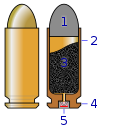
\includegraphics[width=0.5\linewidth]{images/Cartridge_cross_section} 

}

\caption{Image of bullet structure. 1 indicates the bullet, 2 indicates the cartridge casing, 3 indicates the powder, 4 indicates the head of the cartridge casing, and 5 indicates the primer. Glrx (2021).}\label{fig:structure}
\end{figure}

The practice of bullet matching is based on the concept that rifling in a gun barrel can produce uniquely identifying marks on bullets fired from the gun, due to random variation (PCAST, 2016, p. 104).
\authorcol{Rifling is defined as the spiral ridges in a gun barrel that stabilize the bullet, as shown in Figure} \ref{fig:rifling}(baku13, 2005).
\authorcol{The raised areas are known as lands, while the depressed areas are known as grooves.}

\begin{figure}

{\centering 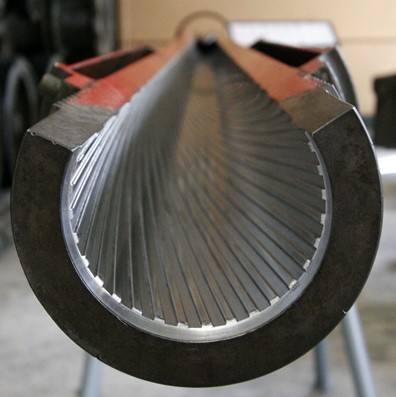
\includegraphics[width=0.5\linewidth]{images/rifling} 

}

\caption{Cross section of a gun. The rifling is the spiral pattern of lands (raised portions) and grooves (indented portions). baku13 (2005).}\label{fig:rifling}
\end{figure}

\authorcol{When a bullet is fired, it travels down the gun barrel and marks from the rifling are scratched into the bullet's surface.
This results in indented areas that correspond to the land impressions, as shown in Figure} \ref{fig:fired}(Gremi-ch, 2009).

\begin{figure}

{\centering 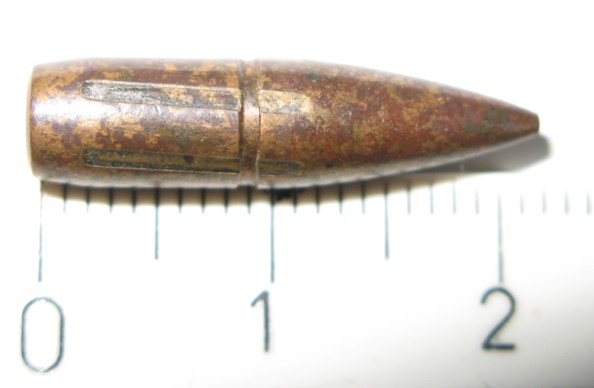
\includegraphics[width=0.5\linewidth]{images/fired_bullet} 

}

\caption{Fired bullet. Indented portion correspond to the gun lands. Gremi-ch (2009).}\label{fig:fired}
\end{figure}

\authorcol{The diagram in Figure} \ref{fig:fireddiagram} from Hare et al. (2017) \authorcol{demonstrates the structure of these land and groove impressions on a bullet.
As there are multiple lands on a gun barrel, this results in multiple land impressions on a fired bullet.}

\begin{figure}

{\centering 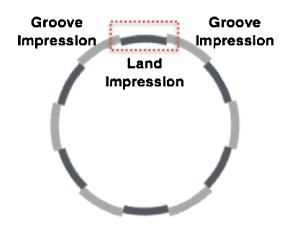
\includegraphics[width=0.5\linewidth]{images/bulletdiagram} 

}

\caption{Diagram of a fired bullet. Hare et al. (2017).}\label{fig:fireddiagram}
\end{figure}

\authorcol{Striation marks, or scratches in the bullet surface caused by the rifling, can be seen on these land impressions, as shown in Figure} \ref{fig:firedland} \authorcol{(provided by} Hare et al. (2017)).
\authorcol{Firearms examiners can compare these striation marks across bullets in order to determine if they were fired from the same gun.}

\begin{figure}

{\centering 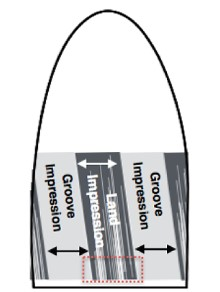
\includegraphics[width=0.5\linewidth]{images/bulletland} 

}

\caption{Side view of a fired bullet, demonstrating striation marks on the bullet's lands. Hare et al. (2017).}\label{fig:firedland}
\end{figure}

\begin{figure}

{\centering 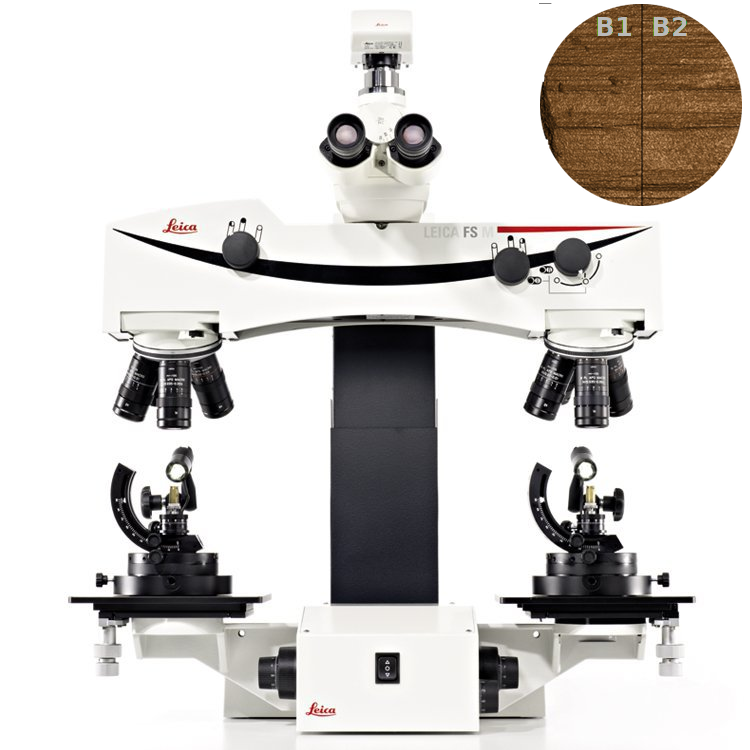
\includegraphics[width=0.5\linewidth]{images/microscope} 

}

\caption{Image of a comparison microscope and aligned bullets}\label{fig:microscope}
\end{figure}

\authorcol{Firearms examiners use comparison microscopes, such as} Figure \ref{fig:microscope}, \authorcol{to compare these striation marks between two bullets, shown in the top right of the figure.}
An early attempt to distinguish guns based on the rifling can be found in two issues of ``The Saturday Evening Post'' from 1925, in an article entitled ``Fingerprinting Bullets''\authorcol{, whose title demonstrates an acceptance of fingerprinting by the public that wouldn't considered by PCAST foundationally valid until an FBI black box study in 2011} (PCAST, 2016, p. 91).
Stout describes the wrongful conviction and subsequent exoneration of Stielow, who was accused of murder (Stout, 1925a).
At the trial where Stielow was found guilty, an expert for the prosecution stated that there were nine abnormalities on Stielow's gun that corresponded with marks on the fired bullet (Stout, 1925a, p. 7).
It was later established that the bullet found at the crime scene indicated the gun was missing a land -- leaving a distinctive pattern -- while the alleged gun showed no such evidence; the alleged gun also showed evidence of not being fired in more than 3 years (Stout, 1925a).

While this trial did not require `uniquely identifying' marks to rule out the alleged weapon (only a mismatch in lands), it motivated Charles Waite to attempt to catalog the manufacturing methods of guns by various companies around the country, with the goal of connecting a gun to its manufacturer.
Waite soon encountered issues due to the multitude of guns produced abroad, as well as ``cheap knock-offs'' with no clear record, making it difficult to trace a gun or bullet to its manufacturer (Stout, 1925b).
While Waite's early attempt to match barrel markings to specific gun brands was focused on the creation of a `database', more recent firearms identification methods have relied on the direct comparison of bullets, such as comparing fired evidence to a suspected gun.

\hypertarget{issues-in-pattern-analysis}{%
\section{Issues in Pattern Analysis}\label{issues-in-pattern-analysis}}

\hypertarget{subjectivity-of-comparisons}{%
\subsection{Subjectivity of Comparisons}\label{subjectivity-of-comparisons}}

\authorcol{A major issue in firearms comparison is the subjectivity of comparisons.
Because there is no objective criteria used to determine what constitutes a 'match' between two samples, experts may view the same evidence and arrive at different conclusions, potentially due to their subjective comparison, differing laboratory procedures, or biases.
Earlier researchers attempted to quantify the bullet matching process through the use of consecutively matching striae, but this process has yet to become standard.}

One of the issues discussed in Stout (1925a) still resonates today: disagreement among experts; this can be especially problematic in countries that use the adversarial judicial system, where experts can testify on the side of the prosecution or the defense.
\authorcol{This could lead to multiple, potentially baised, experts with differing conclusions on the same comparison.}
NRC (2009) states that subjectivity is involved in determining ``sufficient agreement'' among firearms.
This issue is also reflected in Imwinkelried (2020), who suggest that bullet identification is based more on personal experience than on the scientific method.
In plain terms, there is not a set standard for what constitutes sufficient agreement between compared evidence.

Because there is no quantitative score describing the strength of a bullet match, it is possible for experts to use different criterion when making a conclusion about the same evidence.
Disagreement among experts concerning strength of evidence can even be found within a single lab, where experts undergo the same training, use the same equipment and operate under the same procedures, as demonstrated by Montani, Marquis, Egli Anthonioz, \& Champod (2019).
\authorcol{This effect was also present in a bullet comparison study at the Netherlands Forensic Institute, where they found that, of 568 comparison conclusions in a study of the peer review process involving 8 examiners, where the secondary examiner based their conclusion on photos provided by the first examiner, there were 100 disagreements between the two examiners with regards to the strength of evidence, including 6 instances where one examiner found the evidence inconclusive, while the other determined a that the bullets originated from the same source} (Mattijssen, Witteman, Berger, \& Stoel, 2020).

Research has been conducted to better understand the factors that drive firearms examiners to make their conclusions.
The use of virtual comparisons allowed Chapnick et al. (2021) to investigate what examiners considered important when evaluating cartridge cases by including a feature to highlight important aspects of comparisons.
They found that examiners generally tended to highlight the same features when making match conclusions (Chapnick et al., 2021, p. 8).
However, not all examiners who correctly identified the samples used `irregularly shaped marks' to distinguish the known matches: the number was around 60\%-70\% (Chapnick et al., 2021, p. 6).
This is far from a unanimous consensus on important features for determining a match in this type of firearm evidence.
\authorcol{In bullet comparison, Todd Weller discusses the use of consecutively matching striation marks between two bullets as a bullet matching standard that is used by approximately 25\% of examiners, but this standard is not used by either the Association of Firearm and Toolmark Examiners or the Organization of Scientific Area Committees (administered by the National Institute of Standards and Technology)} (Superior Court of California, 2021, p. 98).
\authorcol{While standards for forensic sciences, such as firearm analysis, have been created and published by Scientific Working Groups established by the FBI, these standards are voluntary guidelines that are not uniformly enforced} (NRC, 2009, p. 202).
\authorcol{Thus, the criteria used by experts in firearms analysis varies between individuals.}

Procedural issues may also lead to differing expert opinions across laboratories; one system may not allow an exclusion to be documented if the class characteristics match, while another system may not have such a limitation (Baldwin, Bajic, Morris, \& Zamzow, 2014, p. 6).
In their study, this led to 45 of 218 examiners labeling all different source comparisons as inconclusive, and 96 examiners labeling none of the comparisons as inconclusive (Baldwin et al., 2014, p. 16).
Without a standardized procedure, experts \authorcol{may} evaluate the evidence similarly when comparing two bullets, but must draw different conclusions based on the procedures of their laboratory.
This \authorcol{leads to} in inconsistencies in results based on location, which are compounded with inconsistencies that may arise due to the subjectivity of bullet comparisons.

Aside from the difference in evaluation \authorcol{procedures and identification criterion}, subjectivity can lead to bias in pattern recognition.
The need for an unbiased method of evaluation is aptly demonstrated by the case of the Madrid bombing, in which the FBI incorrectly matched a latent fingerprint to \authorcol{an innocent} individual, despite the use of a verification process (Stacey, 2005).
The individual incorrectly identified was a Muslim from Oregon who had been on an FBI watch list (Kassin, Dror, \& Kukucka, 2013, p. 42).
Kassin et al. (2013) suggest that this incorrect conclusion may relate to confirmation bias, and outline other contributing factors, such as extraneous details, external pressures, and order of presentation.
While this example is based on fingerprint analysis, the same issues of subjectivity are present in bullet matching.

Mattijssen, Witteman, Berger, \& Stoel (2020) \authorcol{studied bias in blind and non-blind peer review.
They found that individuals were significantly more likely to disagree about the strength of evidence in blind peer review (where they were initially unaware of the first examiner's proposed conclusion) than they were in non-blind peer review (where they received the initial examiner's analysis along with the comparison photos).
Of those who disagreed,} Mattijssen, Witteman, Berger, \& Stoel (2020) \authorcol{found that, when it came to discussion between the two examiners to report a final conclusion, the conclusion was more likely to align with the examiner who had the higher perceived professional status (a reporting examiner as opposed to a non-reporting examiner), although the status of the individual was not randomized in this experiment.}
Montani et al. (2019) discuss the importance of independent verification, and how to present results when experts do not agree.
They suggest that, when experts disagree, a third expert should be consulted, and all conclusions should be documented and presented as evidence.
\authorcol{The use of three experts in the case of disagreement in categorical conclusions is also suggested by} Mattijssen, Witteman, Berger, \& Stoel (2020)\authorcol{, although they feel this approach may stifle discussion and peer learning}.

While there are issues in subjective bullet matching, there have been attempts \authorcol{to establish quantifiable standards}.
Biasotti (1959) suggests that statistical methods can be used in order to determine whether two bullets were fired from the same gun.
He concludes that evaluation of individual striation marks \authorcol{(or striae)} is not sufficient, but counting the number of consecutively matching lines may provide enough information to distinguish between matching and non-matching bullets, in the case of the .38 Special Smith and Wesson revolvers used in this study (Biasotti, 1959, p. 37 -- 47).
Biasotti (1959) hoped that such methods may lead to a statistical model for evaluating firearms (47).
The idea of consecutively matching striae (CMS) was addressed again in S. G. Bunch (2000), but a completely standardized or quantifiable method of examination has yet to be developed.
According to Weller, consecutively matching striae is still used today by some examiners; however, this process has not been nationally adopted (Superior Court of California, 2021, p. 98).
Biasotti (1959)'s idea of using consecutively matching lines is used and extended in the bullet matching algorithm developed by Hare et al. (2017).

\hypertarget{scientific-validity}{%
\subsection{Scientific Validity}\label{scientific-validity}}

In recent years, the scientific validity of many forensic science methods have been called into question, as shown in the NRC (2009) and PCAST (2016) reports on feature comparison methods.
General concerns in both reports include foundational evidence for scientific validity, general inability to determine error rates for conclusions, and subjectivity in analysis methods.
Some issues outlined by PCAST (2016) are the circular nature of the identification guidelines \authorcol{put forth by the Association of Firearm and Tool Mark Examiners (AFTE)} and the lack of appropriately designed error rate studies.
AFTE defines sufficient agreement as ``\ldots the examiner being convinced that the items are extremely unlikely to have a different origin'' (PCAST, 2016, p. 104).
Thus, items are classified as having sufficient agreement if they agree sufficiently enough to conclude that they did not come from different sources.
This guideline is in itself subjective - there are no benchmarks for determining what one means by ``extremely unlikely to have a different origin''.
Both NRC (2009) and PCAST (2016) suggest a move away from subjective methods.
PCAST (2016) states the importance of the development of an objective method for firearms comparisons.

These reports also highlighted the lack of studies that produced accurate error rates due to several issues, such as the reporting of inconclusive decisions as well as simple design issues (PCAST, 2016, p. 104 - 112).
For example, Chapnick et al. (2021)'s report does not include inconclusive results as a potential source of error.
They reported three errors (false positives) in their study, and reported a false negative error rate of 0\%, ignoring the wide range of inconclusive decisions.
For participants from the United States and Canada, 38 of 491 comparisons were reported as inconclusive for known matches, while 254 of 693 comparisons were reported as inconclusive for know non-matches (Chapnick et al., 2021, p. 6).
The issues of error rate calculation are addressed by Hofmann, Vanderplas, \& Carriquiry (2021), particularly with regards to whether or not inconclusive decisions should be treated as errors in calculations.
They suggest to not consider inconclusive decisions as errors for the calculation of examiner error rates, used in the lab setting; but to consider inconclusive decisions as errors for process error rates, used for determining if the evidence is relevant enough for judging the guilt of the suspect.
This distinction would allow an examiner to report an inconclusive finding without a negative reflection on their work, as inconclusive decisions are sometimes necessary.
But it would also provide jurors with relevant information for evaluating the reliability of firearms evidence.

In another evaluation of inconclusive results, Dror \& Scurich (2020) describe different ways in which inconclusive results are produced.
They differentiate between inconclusive decisions based on the amount of evidence present; an examiner reaching an inconclusive decision when there is not sufficient evidence to reach a conclusion would be correct, whereas an examiner reaching an inconclusive decision when there is sufficient evidence to reach a conclusion would be incorrect.
This definition relies on \authorcol{the hitherto undetermined standard of the quantifiable} amount of evidence necessary to reach a conclusive decision.
By failing to distinguish between correct and incorrect inconclusive decisions in research studies, examiners may opt for the inconclusive choice on hard conclusive comparisons, resulting in error rates that are only valid for easy comparisons when inconclusive decisions are not considered an error(Dror \& Scurich, 2020, p. 336).
Dror \& Scurich (2020) would consider those inconclusive choices to be ``incorrect'' - there is enough evidence to reach a conclusion.
Similarly, another potential error would be the examiner reaching a conclusive decision when there is not sufficient evidence to reach a conclusion (Dror \& Scurich, 2020, p. 334).
This delineates conclusion and errors into distinct categories, which are not seen in error rate studies.

Both inconclusive and conclusive results for the same analysis cannot be correct -- there either is enough evidence to make a conclusion, or there is not enough evidence to make a conclusion; to say otherwise may deflate actual error rates (Dror \& Scurich, 2020, pp. 334--335).
Dror \& Scurich (2020) indicate that this inconclusive issue is more prominent in studies than in casework, as inconclusive decisions are more common in error rate studies.
Hofmann et al. (2021) \authorcol{also found that examiners made far more inconclusive decisions when the ground truth was a non-match compared to a match when using the AFTE range of conclusions.}
However, this distinction between correct and incorrect decisions are not commonly made in studies due to a lack of a quantifiable method for separating the two categories, leading to inconclusive decisions lowering the error rate in some studies.

\authorcol{In other studies, it is impossible to calculate an accurate error rate based on the study design - if examiners are asked to compare unknown bullets to multiple known sources in a set, we do not know if the examiner compared each unknown bullet to all of the knowns in order to reach a conclusion, or if they stopped performing comparisons with the unknown bullet once they found the matching known; this limits information on how often examiners correctly identify different source comparisons} (Hofmann et al., 2021).
As Hofmann et al. (2021) \authorcol{state, this study design makes it impossible to calculate error rates for different-source comparisons.}

Other issues in the computation of error rates include the use of closed set studies, which result in significantly lower rates of inconclusive decisions and false positives (PCAST, 2016, p. 109). In closed set studies, the source gun is always present, and examiners are asked to match a set of known bullets to a set of unknown bullets - allowing for them to use a process of elimination to make matches; conversely, open set studies do not include all source guns (PCAST, 2016, pp. 108--110).
The Ames Laboratory study is described by PCAST (2016) as an appropriate closed set black-box study (111).
These types of analyses are classified as black-box studies because reported match results are based on an examiner's subjective opinion rather than a list of objective steps (PCAST, 2016, p. 5).
When comparing closed-set studies to non closed-set studies, PCAST (2016) found that closed-set studies had a much lower rate of inconclusive decisions as well as false positives (111).

\hypertarget{scale-of-conclusions}{%
\subsection{Scale of Conclusions}\label{scale-of-conclusions}}

This debate regarding scientific validity continues to this day, as Vanderplas, Khan, Hofmann, \& Carriquiry (2022) shows.
In this declaration, they discuss the current issues with error rate studies, in which they conclude that, until valid error rate studies have been conducted, they cannot support the use of firearms analysis in the courtroom (Vanderplas et al., 2022, p. 10).
Others have called to scale back conclusions that attest to ``individualization'' in the courtroom due to the inability to tie a specific piece of evidence to a specific source, to the exclusion of all other sources (Imwinkelried, 2020; NRC, 2009).
There has been some resistance to scaling back conclusions, however, as demonstrated in a memo sent out by Jim Agar II, an FBI attorney.
They stated that less conclusive language would not be truthful on the part of the firearm expert and to ask firearms examiners to use this language would result in perjury (Agar II, 2021), despite the reliance on subjective methods with unclear error rates.

There has also been some push back against the conclusions of PCAST (2016), as shown in OSAC (2016) (provided by the Firearms and Toolmarks subcommittee.
According to Davis \& Baker (2014), the Organization of Scientific Area Committees (OSAC) subcommittees are ``generally composed of 70\% practitioners, 20\% researchers, and 10\% research and development technology partners and providers''.
OSAC (2016) argue that a false positive error rate is not necessary for determining foundational validity, and that closed set error rate studies are fine for calculating error rates.
OSAC (2016) also suggests that PCAST (2016) ignores the importance of peer review in studies that instruct firearms examiners to work alone, and that black box studies may not properly reflect casework.
However, in order to accurately represent casework, blind testing (where the examiner does not know they are being tested) would be needed - but due to logistical issues and case load, this may not be feasible (PCAST, 2016, p. 59).
OSAC (2016) argues that AFTE language is not circular - the basis of a practical impossibility is based on knowledge of best known non-matches conveyed through training.
Here decisions are based on ``knowledge and experience'', which does not counteract the subjective nature of this decision making.
Despite these disagreements OSAC (2016) also promotes the use of more objective methods.

These differing views are represented in Swofford \& Champod (2022).
Swofford \& Champod (2022) interviewed 15 individuals with a range of expertise in forensic science and the court system in order to assess their feelings about the use of algorithms and the presentation of probabilistic reporting, as opposed to categorical reporting and traditional analysis methods.
They found that prosecutors interviewed supported the use of match terms such as ``identification'' and ``individualization'' instead of probabilistic terms, but two of the prosecutors also rejected the use of terms that convey ``absolute certainty'' (7).
All participants felt that that examiner testimony should accurately reflect scientific limitations, although there was not a consensus on whether this practice was in fact followed in the courtroom - defense attorneys felt that the examiners usually do not uphold this expectation, while lab managers expressed frustration on the part of the court (19).
The scale to which firearm evidence is used in the courtroom is rather contentious, and views may differ based on occupation.

In general, individuals want to guarantee that the information presented in the courtroom is accurate and valid, without causing too much imbalance between the limitations and the categorical conclusion.
However, there isn't agreement on where the balancing point between these two factors are - somewhere between giving too much credit with a match of ``absolute certainty'', and introducing unfounded reasonable doubt by overstating the limitations.
If accurate numerical information on error rates or an objective method of evaluation that can be described to the court were available, it may be possible to have factual statements of limitations and scope of evidence that both sides of the argument would find satisfactory.
In an investigation on the effect of the inclusion of error rate on either voice or fingerprint evidence, B. L. Garrett, Crozier, \& Grady (2020) found that the inclusion of an error rate reduced convictions for fingerprint evidence presented categorically, but had no effect in the case of voice comparison (a less established science) or when the fingerprint comparison was presented as a likelihood ratio.
They state, ``This suggests that error rate information is particularly important for types of forensic evidence that people may assume are highly reliable.'' (1206).
It seems that including error rates for evidence methods seen as reliable may call into question some assumptions participants make about the science, resulting in a closer consideration of the facts presented at trial.

Quantifying both the limitations in terms of error rates and the analysis method with set cutoffs would leave the language used by experts when presenting evidence as a variable that can be manipulated.
While there is much debate over the language used in these conclusions, B. Garrett \& Mitchell (2013) found that the specific language used to describe the strength of the match (when a match was present) had little effect on participants' judgement of guilt. They tested 11 different forms of match language, such as `individualization', `match', or `very likely that the defendant was the source', as well as language that included match conclusions `bolstered' by certainty or likelihood language (B. Garrett \& Mitchell, 2013, p. 489).
McQuiston-Surrett \& Saks (2009) also found that there was not a significant difference in participants' view of the likelihood the defendant committed the crime when the examiner presented the conclusion as a `match' compared to presenting the conclusion as `similar in all microscopic characteristics.'
B. Garrett \& Mitchell (2013) suggests that this lack of difference may relate to the overall view of firearms evidence as reliable, meaning that even a weak match basically boils down to being a match in the eyes of the participants (507).
They also found some tempering effect of the expert admitting the possibility that their conclusion was made in error (507).
Thus, the use of accurate error rates may moderate the reliability of experts for a more considered weighing of evidence.
In fact, in the Ninth Judicial Circuit Court, there are jury instructions regarding the need for juries to treat firearms and other `expert' testimony in the same manner as other opinion testimony, in which they must decide how much weight the testimony should receive (United States Courts for the Ninth Circuit, 2019). United States Courts for the Ninth Circuit (2019) also suggest to avoid labelling such testimony as expert testimony, since it may cause jurors to give the testimony undue weight.
One way to fix these issues of subjectivity is by developing a more objective method of evaluation.
One objective method introduced to the forensic sciences is bullet matching algorithms, such as the one described in Hare et al. (2017).

\hypertarget{quantitative-methods}{%
\section{Quantitative Methods}\label{quantitative-methods}}

\hypertarget{bullet-matching-algorithm}{%
\subsection{Bullet Matching Algorithm}\label{bullet-matching-algorithm}}

This bullet matching algorithm was developed by Hare et al. (2017) and uses a random forest in order to determine a match score (Hare et al., 2017, p. 2352).
This algorithm can be described as follows:

The algorithm first takes a 3D scan of the two bullet lands, then identifies a cross section, or a stable area of the bullet land that can be used in comparison.
This cross section is used in order to identify the signatures of the bullets, or a 2D line that captures the marks scratched onto the bullet's surface.
First the shoulders (the raised area on either side of the scratched pattern) must be removed from the cross section.
Then a loess smoothing is applied twice in order to remove the curvature of the bullet.
What is left is the bullet land's signature (which will show the peaks and valleys produced by the barrel of the gun).
The two signatures are compared using a variety of attributes, such as consecutively matching striae and the relative height of the peaks/valleys, as shown in Figure \ref{fig:signaturecompare}.

\begin{figure}

{\centering 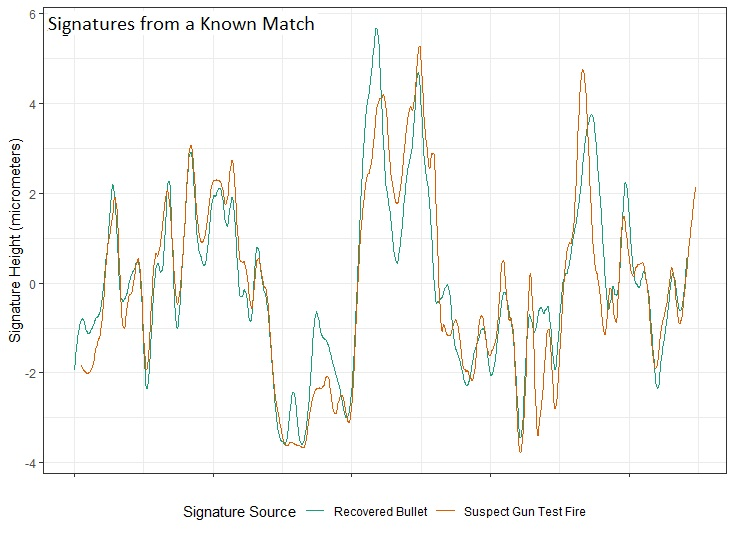
\includegraphics[width=0.49\linewidth]{images/Match_Signatures} 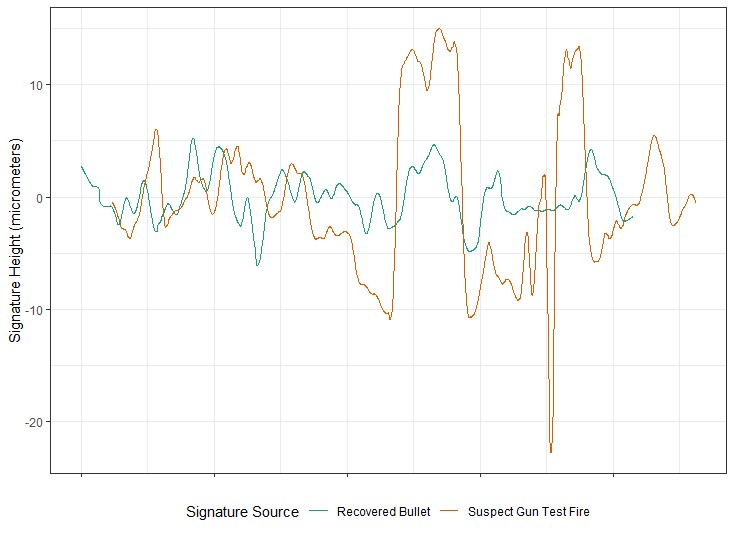
\includegraphics[width=0.49\linewidth]{images/K995_NoMatch_Signatures} 

}

\caption{Left image depicts two matching signatures, while the right image depicts two non-matching signatures. These were generated by the author.}\label{fig:signaturecompare}
\end{figure}

A random forest is used to compare the two signatures and come up with a match score for the lands.
Lands are then aligned across the bullet for the maximal random forest score, and this number would be considered the match score for the bullet.
Figure \ref{fig:gridcompare} shows two grids of land match scores computed in two different bullet comparisons.

\begin{figure}

{\centering 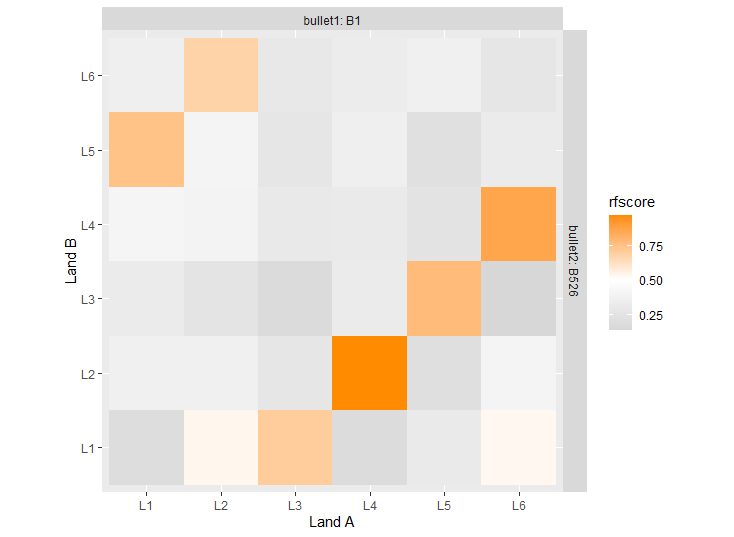
\includegraphics[width=0.49\linewidth]{images/F526_Match_SingleGrid} 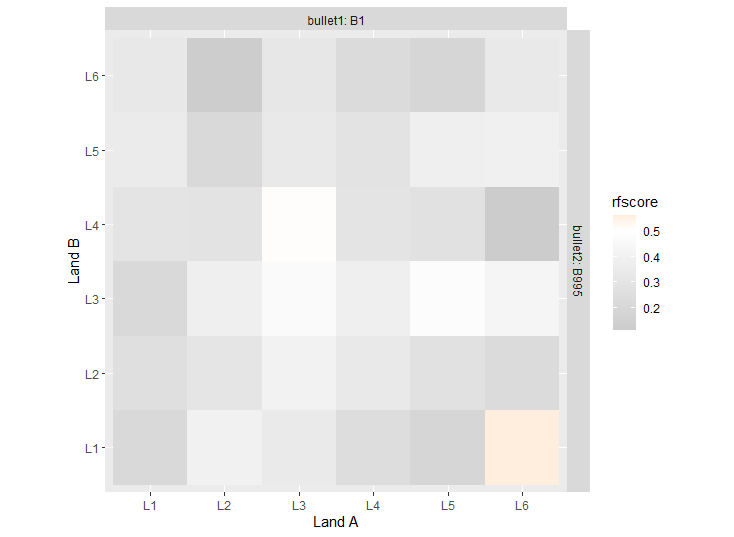
\includegraphics[width=0.49\linewidth]{images/K995_NoMatch_SingleGrid} 

}

\caption{Left image depicts two matching bullets (indicated by high land-to-land match scores in a diagonal formation), while the right image depicts two non-matching bullets.}\label{fig:gridcompare}
\end{figure}

In multiple tests, it was found that the algorithm is able to successfully distinguish between known matches and known non-matches without the use of an inconclusive decision (Vanderplas, Nally, Klep, Cadevall, \& Hofmann, 2020, p. 10).
If the bullet is not fit for algorithmic comparison, then an `inconclusive' result may still be reached.
This may be the case for gun types that have not been tested for the algorithm.
The use of an algorithm allows for quantification of bullet matching, for cases where the algorithm has been verified.

There are some concerns about implementing algorithms for forensic evidence in the courtroom, due to the issue of explaining complex methods to jurors.
B. L. Garrett \& Rudin (2023) explain one main issue that may result from ``black box'' algorithmic methods: the results from the algorithm may not be accurate, and this may be difficult to discern when individuals do not understand the method used.
They instead suggest the use of ``glass box'' methods, where the algorithm's model is interpretable (people can see how it works, and what information is used to make decisions).
B. L. Garrett \& Rudin (2023) state that ``\ldots interpretability is particularly important in legal settings, where human users of a system\ldots{} cannot fairly and accurately use what they cannot understand.''.
This brings up a particularly salient point in jury trials - jurors should understand the pattern comparison process if they are making decisions based on its results.
In a combination of computerized results and human interpretation, Montani et al. (2019) suggest presenting the algorithm as a ``second independent expert'' whose comparison and conclusion can be compared to and presented alongside the examiner's.
Supplementing the decision of the forensic expert with an algorithm would allow for verification of results in two independent methods.
The three laboratory managers interviewed by Swofford \& Champod (2022) suggested using algorithms as a supplement to the forensic examiner (6), similar to Montani et al. (2019)'s suggestion.
The three prosecutors varied in their feelings of algorithms in the courtroom: one thought that they would add unnecessary complications, while two suggested that the algorithms may be useful for the forensic expert (Swofford \& Champod, 2022, p. 8).
The three defense attorneys, as well as the three judges, also supported the use of algorithms as empirical evidence, while stating concerns of transparency (Swofford \& Champod, 2022, pp. 10--13).
Three academic scholars supported the use of algorithms, so long as the algorithms can be understood, have been validated, and do not include factors that may cause systematic biases (Swofford \& Champod, 2022, p. 16).
Swofford \& Champod (2022)'s study demonstrates the variety of opinions on algorithm implementation throughout forensic science, although most support the use of algorithms.

\hypertarget{quantitative-results}{%
\subsection{Quantitative Results}\label{quantitative-results}}

Quantitative methods of examination can lead to quantitative results.
In this case, the quantitative results are in the form of a match score, but in other cases, results may be presented as a likelihood ratio.
For example, John Song, Chen, Vorburger, \& Soons (2020) proposed a likelihood approach for a cartridge case comparison method that uses congruently matching cells.
This is a change from the match language usually used by forensic examiners, but these likelihood ratios may have some benefit.
Marquis et al. (2016) suggest that the use of a likelihood ratio requires examiners to consider what they are including when weighing the strength of evidence, and provides a value that can be consistent across disciplines (4).
This quantitative approach, even while conducting a subjective evaluation, is meant to prevent examiners from being biased by information provided outside of their direct examination (S. Bunch \& Wevers, 2013, p. 223).
The approach also asks examiners to consider both the null and alternative hypotheses, and may make it less likely for either the examiners or jurors to transpose the conditional, which may happen in the case of reporting probabilities (Evett, 1998; Marquis et al., 2016, p. 3).

As an example of transposing the conditional, suppose an examiner were comparing a bullet from the suspect's gun to a bullet recovered from the crime scene.
The examiner may find that there is significant agreement between the two bullets.
They may then conclude that ``the probability of seeing such significant agreement between the two bullets \emph{given that another gun fired the bullet at the crime scene} is small''.
In this case, the examiner is making a statement regarding the amount of agreement between the two bullets (P(Correspondence\textbar Different Source)).
If the conditional is transposed, the statement would become ``the probability that another gun fired the bullet at the crime scene \emph{given the significant agreement between the two bullets} is small'' (P(Different Source\textbar Correspondence)).
Here, the conditional part of the statement has been switched, so that the examiner is making a statement regarding the gun being fired at the crime scene instead of a statement with regards to the bullet comparison.
By stating a likelihood ratio, such as ``the bullet comparison provides strong support for the proposition that the two bullets came from the same gun rather than the proposition that the two bullets came from different guns'', both the null and alternative hypothesis are clearly stated, and the focus of the statement is on the bullet comparison, rather than the gun's presence at the crime scene.

As shown above, the likelihood ratio directly compares the null and alternative hypotheses in a case, which is not accomplished by considering a single probability (Nordgaard, Ansell, Drotz, \& Jaeger, 2012, p. 6).
Likelihood ratios also allow for the integration of evidence from multiple sources, and individual likelihood ratios may be multiplied together to calculate an overall likelihood ratio.
Meuwly, Ramos, \& Haraksim (2017) suggested guidelines for validating both score- and feature-based likelihood ratio methods, so this form of result presentation could be more widely accepted.
These methods included validation criteria for all variables considered in a likelihood ratio, where validation criteria can be considered in several ways: a comparison with current ``state of the art'' methods, detection error trade-off graphs to measure discriminating power, and performing validation on a validation data set.

\hypertarget{explainability-in-the-courtroom}{%
\subsection{Explainability in the Courtroom}\label{explainability-in-the-courtroom}}

One roadblock in the use of quantitative methods and results, such as likelihood ratios, in the forensic sciences is the necessity to explain such methods to jurors so that they can understand the method and results well enough to make informed decisions in court cases.
Association of Forensic Science Providers (2009) stated that opinions and conclusions should be expressed in likelihood ratios when outlining guidelines for forensic experts (163).
Participants in Swofford \& Champod (2022) expressed concern that probabilistic reporting (as opposed to categorical reporting) would be confusing and easily misinterpreted, when compared to the alternative of categorical reporting (18).
In order to gauge how quantitative methods are perceived in the courtroom, we can consider fingerprint and DNA analysis.
B. Garrett, Mitchell, \& Scurich (2018) studied the use of FRStat for fingerprint matching in the courtroom.
The FRStat language presented to the study participants is as follows: ``The probability of observing this amount of correspondence is approximately {[}XXX{]} times greater when the impressions are made by the same source rather than by different sources'' (language from Defense Forensic Science Center, 2018).
B. Garrett et al. (2018) used ratios from 10 times greater to 100,000 times greater, and found that the likelihood that the subject committed the crime according to the participants did not change significantly.
This demonstrates that potential jurors may have trouble accurately interpreting statistical results, including likelihood ratios.

In DNA research, Koehler (2001) found that participants were more likely to believe the subject was the source of the DNA when presented with a probability instead of a frequency.
When asked about how many individuals would match DNA for a given match proportion in a population of 500,000, 60.7\% of participants who received a frequency and 42.1\% of individuals who received a probability answered correctly (Koehler, 2001, p. 503).
When asking these individuals to determine the guilt or innocence of a suspect, the percentage of participants who correctly interpreted the DNA results seems relatively low.
Jurors are also prone to find evidence to be weaker when frequencies are presented as whole number (1 out of 100,000) compared to a decimal number (0.1 out of 10,000), even though the frequencies represent the same value (Koehler \& Macchi, 2004, p. 544).
These studies show that individuals struggle with interpreting numerical results, and assigning appropriate weight to likelihood ratios.

In addressing these issues of interpretation, attempts have been made to assign a verbal scale to be used alongside a likelihood ratio, such as the European recommendations for reporting forensic science \authorcol{put forth by the European Network of Forensic Science Institutes} (ENFSI, 2016).
A sample of phrasing from their recommended scale has been recreated in Table \ref{tab:enfsi}.
Verbal values range from no support to extremely strong support, and correspond to a numerical output.
This type of scale would present jurors with both the quantitative result as well as a brief interpretation, so they are not solely relying on their own perception of what the likelihood ratio qualitatively means.
It also offers a numerical scale that may encourage consistency across examiner reports.

\begin{longtable}[]{@{}
  >{\centering\arraybackslash}p{(\columnwidth - 2\tabcolsep) * \real{0.2016}}
  >{\centering\arraybackslash}p{(\columnwidth - 2\tabcolsep) * \real{0.7984}}@{}}
\caption{\label{tab:enfsi} Sample language from ENFSI (2016) (17)}\tabularnewline
\toprule\noalign{}
\begin{minipage}[b]{\linewidth}\centering
Likelihood Ratio
\end{minipage} & \begin{minipage}[b]{\linewidth}\centering
Verbal Equivalent
\end{minipage} \\
\midrule\noalign{}
\endfirsthead
\toprule\noalign{}
\begin{minipage}[b]{\linewidth}\centering
Likelihood Ratio
\end{minipage} & \begin{minipage}[b]{\linewidth}\centering
Verbal Equivalent
\end{minipage} \\
\midrule\noalign{}
\endhead
\bottomrule\noalign{}
\endlastfoot
1 & The forensic findings do not support one proposition over the other \\
2 - 10 & The forensic findings provide weak support for the first proposition relative to the alternative \\
10 - 100 & \ldots provide moderate support for the first proposition rather than the alternative \\
100 - 1,000 & \ldots provide moderately strong support for the first proposition rather than the alternative \\
1,000 - 10,000 & \ldots provide strong support for the first proposition rather than the alternative \\
10,000 - 1,000,000 & \ldots provide very strong support for the first proposition rather than the alternative \\
1,000,000 and above & \ldots provide extremely strong support for the first proposition rather than the alternative \\
\end{longtable}

A similar scale is also suggested by Evett (1998), with verbal values of ``Limited support'', ``Moderate support'', ``Strong support'', and ``Very strong support'' (201).
These values approximately correspond to the scale above, but consists of fewer categories.
Marquis et al. (2016) suggest against providing the full verbal scale to participants, because participants may use other terms on the scale in order to orient the likelihood ratio in comparison to the full scale (7).
However, this ability to orient relative to other values may assist jurors in accurately judging the strength of evidence presented.

While verbal scales are useful for clarification, individuals may not always interpret them consistently.
For example, Budescu \& Wallsten (1985) asked participants to rank common probabilistic words (such are ``rarely'' or ``usually'') on three separate occasions, finding that individuals typically gave consistent rankings across time points, but there was variation in rankings between individuals.
In an earlier study, Lichtenstein \& Newman (1967) asked individuals to assign numerical probabilities to probabilistic words, finding that eight of the eleven mirror terms (such as ``quite likely'' and ``quite unlikely'') demonstrated asymmetry - positive terms (such as likely) scored lower than their mirrored negative terms (unlikely). For example, ``quite likely'' and ``quite unlikely'' had median values of 0.8 and 0.1, respectively (Lichtenstein \& Newman, 1967, p. 564).

Martire, Kemp, Watkins, Sayle, \& Newell (2013) studied the use of a verbal scale similar to ENFSI (2016) in a courtroom setting, in the case of shoe print evidence.
They found a ``weak evidence effect'', in which findings that provided ``weak support'' for the proposition that the defendant's shoe left the print resulted in decreased likelihood scores of guilt, compared to likelihood scores collected before the introduction of forensic evidence.
Martire et al. (2013) did not find this trend when the evidence was presented numerically as a likelihood ratio; in this case, participants tended to think of the defendant as more guilty after hearing the forensic evidence (as expected).
They did not, however find that the reverse was true: those who received ``weak support'' for the proposition that the defendant did not leave the shoe print resulted in increased likelihood scores in favor of innocence, as expected.
Martire et al. (2013) hypothesize that this demonstrates that the participants are engaging in a ``criminal justice perspective'' by weighting the evidence toward the defendant's innocence (since the burden of proof rests on the prosecution).
This inconsistency of interpretation between the numerical scale and the verbal equivalent may act as evidence against implementation of a solely verbal scale.

Examiners also show evidence of inconsistency in scale interpretation.
Mattijssen, Witteman, Berger, Brand, \& Stoel (2020) asked examiners to use a verbal scale for degree of similarity and support when digitally comparing cartridge cases.
When using a verbal scale for degree of similarity/support, Mattijssen, Witteman, Berger, Brand, et al. (2020) found that the between-subject and within-subject reliability was moderate to high (11).
Mattijssen, Witteman, Berger, Brand, et al. (2020) asked 10 examiners who regularly used likelihood ratios to provide both a verbal degree of support along with a likelihood ratio.
They found that the verbal degrees of support were in general an overestimation when compared to the likelihood ratios (8).
While this is a small non-representative sample, it suggests that verbal scales do not always correspond to quantitative scales across subjects.
Thompson \& Newman (2015) investigated the amount of weight participants gave either DNA or shoeprint evidence when it was presented as a likelihood ratio, verbal equivalent, or random match probability.
While individuals updated their response as expected when the strength of evidence was changed in all cases of the DNA condition, participants did not produce significantly different estimates when shoe print evidence was presented as a likelihood ratio or verbal equivalent, but they did produce different estimates in the case of the random match probability.
These results indicate that participants may weigh evidence differently depending on the presentation method.
Thompson \& Newman (2015) hypothesize that the difference between the DNA results and the shoe print results may stem from the perception of DNA analysis as highly scientific.
By combining the quantitative analysis with a verbal translation, it may be possible to present quantitative results in a manner that is understood consistently by laypeople.

This mix of quantitative language alongside more categorical terms is supported by subjects in Swofford \& Champod (2022).
Almost all participants expressed concerns about the interpretation of the probabilistic language, and many recommended a combination of both methods (Swofford \& Champod, 2022).
The prosecutors interviewed thought that match language was sufficient by itself, and did not wish to complicate testimony with probabilistic language (Swofford \& Champod, 2022, p. 8).
McQuiston-Surrett \& Saks (2009) studied the use of match language versus probabilities with both judges and juries.
Both groups assigned higher probabilities to the defendant committing the crime when presented with qualitative evaluation or a single probability for the hair comparison, as compared to frequency methods of reporting.
McQuiston-Surrett \& Saks (2009) found that participants were more sure of the guilt of the defendant when qualitative language was used as opposed to a subjective probability.
While match language may give jurors more confidence, it could have the effect of shifting the consideration of evidence from the jury (who in a quantitative approach would need to determine whether or not they feel a likelihood ratio is large enough to indicate that the subject is the source) to the forensic expert, who can declare a match.

\hypertarget{demonstrative-evidence}{%
\subsection{Demonstrative Evidence}\label{demonstrative-evidence}}

Aside from result language or scales used, another important factor in jury decision making is demonstrative evidence.
Images can supply helpful context in describing complex forms of analysis, but they may also introduce bias in the form of ``truthiness'', a\authorcol{n official} term introduced by comedian Stephen Colbert.
He described truthiness as the quality of something \emph{seeming} true (Colbert, 2005).
In this video, Colbert talks about ``thinking with your head vs.~knowing with your heart'', where some information may feel true, regardless of the facts.
Bornstein \& Greene (2011) found a ``truthiness'' effect in the courtroom - jurors tend to remember evidence that align with their previous beliefs (65).
\authorcol{This concept can apply to images that make people more likely to feel like a statement is true, even when they do not contribute new evidence.}
Kellermann (2013) suggests that the truthiness or ``falsiness'' of non-probative visual images should be carefully considered before using images in the courtroom ``\ldots both to prevent backfire effects and to capitalize on every possible tactic that can be used to persuade jurors\ldots{}'' (40).
While the concept of truthiness can be used to benefit either side in an adversarial justice system, trial outcomes should be based on factual evidence, rather than feelings that evidence is factual.
In the case of images in trials, it is important to balance the benefit of providing additional information to the jury via images without increasing truthiness.

The impact of photos on an individual's perception can be rather large, as investigated by Cardwell, Henkel, Garry, Newman, \& Foster (2016).
They asked individuals to ``give'' or ``take'' food from an animal, represented by a word.
Subjects were later asked to identify whether or not they gave food to an animal -- either accompanied by an image or not.
Individuals were more likely to say that they gave food to an animal if it was accompanied by an image (Cardwell et al., 2016, p. 887).
They found that images had an effect for positive associations such as giving food, but not negative associations such as taking food (Cardwell et al., 2016, p. 883).
In this case, the use of images may make it easier for individuals to visualize a scenario (giving food), and thus makes them more likely to remember the event - whether it happened or not.

In a study of perception, McCabe \& Castel (2008) presented a variety of graphics alongside articles relating to cognitive neuroscience.
The graphics all contained the same information, which was already presented the accompanying article.
They found that participants gave higher ratings of scientific reasoning to articles that included a brain image with activated areas, as opposed to a bar chart, topographical brain graphic, or no graphic.
Participants were also more likely to agree with the conclusion of an article when the brain image was present, compared to when it was absent.
Although the information presented in the articles did not change throughout these conditions, the brain image appears to add more ``truthiness'' to the articles, causing individuals to find them more scientific than articles with other graphics or no graphics.

In the courtroom, studies have been conducted to evaluate the effect of images of the brain.
Gurley \& Marcus (2008) studied the use of brain images when arguing the defendant is not guilty by reason of insanity.
In a study on introduction to psychology university students, they found that the inclusion of images showing a brain lesion increased the odds of the participants finding the defendant not guilty by reason of insanity.
MRI scans were presented with additional information regarding impulse control for the damaged area, so the effect may not be caused by the images themselves but rather by the additional information.
Schweitzer et al. (2011) investigated whether images of the brain presented alongside expert testimony with regards to a mental disorder effected the participant's verdict of the defendant's mental state.
In this case, no additional information was provided alongside the neuroimage, allowing the effect of the image itself to be studied.
They found that the inclusion of neuroimages did not significantly effect the judgement of the participants.
The influence of images on individuals remains unclear, and may be situationally dependent.

\hypertarget{response-methods}{%
\section{Response Methods}\label{response-methods}}

There are many different ways to measure participant responses, each of which may affect the accuracy with which the response reflects the construct that we wish to measure (Groves et al., 2009).
Verbal scales, such as those used in the ENFSI guidelines described in the last section, are often used to record participant responses.
Likert scales can be used to evaluate several factors, such as the reliability, understanding, and scientific quality of the forensics expert, the algorithm, and the testimony in general.
It is therefore important to ensure that participants' views are accurately recorded with Likert type scales, which can vary in the number of categories used.
Several researchers found that the 7-point scale may perform or represent the participants' true views better than the 5-point scale (Finstad, 2010; Joshi, Kale, Chandel, \& Pal, 2015).
While Groves et al. (2009) recommends using a 5 or 7-point Likert scale with a label for every scale point for attitude questions, participants often preferred more categories, such as 7, 9, or 10 (Komorita \& Graham, 1965; Preston \& Colman, 2000).
However, Preston \& Colman (2000) found that reliability decreased with more than 10 categories.
This indicates that 7, 9, or 10 point scales should be adequate for reliable responses that accurately represent the participant's views.
In addition, DeCastellarnau (2018) found that asking participants to respond to specific items (such as reliable - unreliable) is preferred over using a generalized agree - disagree scale in terms of measurement quality, cognitive effort, and bias.

Other methods have also been used to evaluate participant responses, such as asking participants to give a likelihood ratio or a probability of guilt.
Thompson, Kaasa, \& Peterson (2013) asked participants rate the chance of guilt on a scale from: with values generally on a log 10 scale (ex. 1 in 100; 1 in 1,000); a middle value of a fifty-fifty chance; and extreme values of ``Certain to be guilty'' and ``Impossible that he is guilty''.
They compared results from participants to Bayesian conditional probabilities based on provided likelihoods of a match and error rates in order to consider how much weight participants were giving DNA evidence.
Their results mainly showed no significant difference between Bayesian and participant estimates (meaning that the estimates were ``in the right ballpark''), with some conditions producing estimates either greater than or less than what was expected.

In another study of the relationship between how examiners present evidence (likelihood ratio, verbal equivalent, or random match probability), Thompson \& Newman (2015) applies the same multiple choice scale for selecting the chance that the defendant committed the crime for half of the participants, while the other half of the participants were asked to supply how many more times likely it was that the defendant was guilty as compared to not guilty, or vice versa (based on a response scale found in Martire et al. (2013)).
The likelihood statement was worded as follows: ``Based on the available evidence I believe it is \_\_\_ times more likely that Mr.~Kelly is guilty than not guilty.'' (Thompson \& Newman (2015), 5).
In comparing responses from these two scales, Thompson \& Newman (2015) found that individuals were more likely to give higher estimates on the categorical log scale than when they were asked to provide a likelihood - resulting in the categorical log scale being more consistent with the expected result when using Bayesian methods of calculation.
This indicates an inconsistency in results based on the response method used.

\hypertarget{conclusion}{%
\section{Conclusion}\label{conclusion}}

In order to ensure that the US justice system is just, we must be confident that the evidence presented in the courtroom is scientifically valid, and that the evidence is presented in a way that gives jurors the ability to appropriately judge its strength.
This includes the use of accurate error rates as well as quantitative responses.
One way to facilitate error rate calculation and quantitative results is through the use of algorithmic or statistical methods.
These methods must, however, be explained in a manner that is understandable to those without a statistical background, while limiting any of the potentially biasing effects of ``truthiness''.

\hypertarget{study1}{%
\chapter{Jury Perception of Bullet Matching Algorithms and Demostrative Evidence}\label{study1}}

\hypertarget{background}{%
\section{Background}\label{background}}

\hypertarget{firearms-examiners}{%
\subsection{Firearms Examiners}\label{firearms-examiners}}

The foundational belief in bullet comparisons as a form of identifying evidence is that guns can leave unique striation marks on a bullet as an artifact of the rifling process (PCAST, 2016, p. 104).
Striation marks are left on portions of the bullets known as ``lands'', due to contact with the rifling as the bullet is fired.
These marks are compared by examiners across bullets in order to identify if bullets were fired from the same source.
These examinations are subjective, as they are based on the firearms examiner's experience and judgement (NRC, 2009, p. 153).
This can lead to issues of bias in analysis (Kassin et al., 2013). In 2019, the PCAST report highlighted common issues with traditional bullet matching methods, such as the lack of appropriately designed error rate studies and the circular nature of AFTE's bullet matching guidelines (PCAST, 2016, pp. 104--112).
Issues in error rate studies have been discussed in several articles (Dror \& Scurich, 2020; Hofmann et al., 2021).
PCAST emphasizes the importance of the development of an objective method for firearms comparisons (PCAST, 2016, p. 113).
The use of an automatic, objective method would contribute to quantifiable presentation of evidence and would lower the effort required to identify the method's error rate.

\hypertarget{bullet-matching-algorithm-1}{%
\subsection{Bullet Matching Algorithm}\label{bullet-matching-algorithm-1}}

Following PCAST's publication, many methods of statistical matching have been developed and evaluated, such as Hare et al. (2017), Vanderplas et al. (2020), J. Song et al. (2012), and Vorburger, Song, \& Petraco (2015).
In this study, the bullet matching algorithm used was developed by Hare et al. (2017).
The algorithm can briefly be described as follows:

\begin{enumerate}
\def\labelenumi{\arabic{enumi}.}
\tightlist
\item
  A 3D scan is taken of each bullet land (containing striation marks to be compared), a stable cross-section is extracted, and shoulders (without relevant striation marks) are removed, as in \ref{fig:shoulder}, an image from Hare et al. (2017).
\end{enumerate}

\begin{figure}
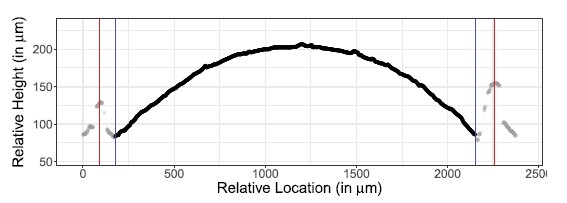
\includegraphics[width=\linewidth]{images/shoulder} \caption{The land is shown in the center. Shoulders are shown outside of the vertical lines.}\label{fig:shoulder}
\end{figure}

\begin{enumerate}
\def\labelenumi{\arabic{enumi}.}
\setcounter{enumi}{1}
\tightlist
\item
  A smoothing function is applied twice in order to extract the signature, a pattern of high and low points on the bullet's surface corresponding to the striation marks.
  The signature can then be compared to land signatures from other bullets, as in \ref{fig:signature}.
\end{enumerate}

\begin{figure}
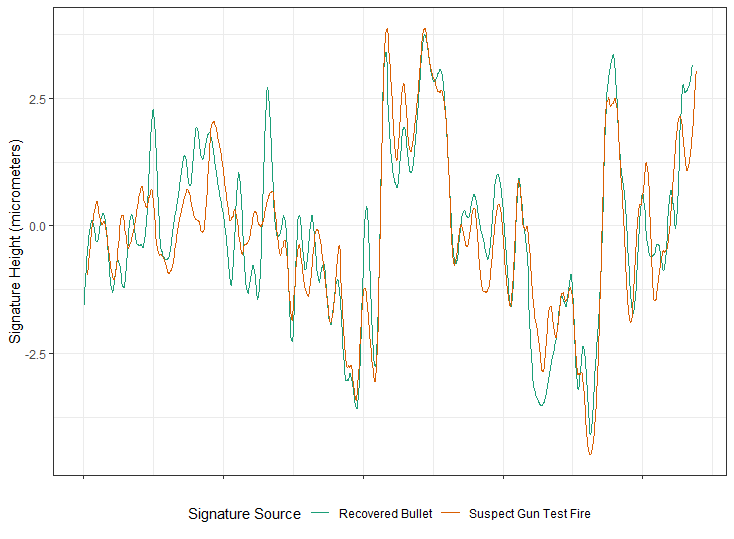
\includegraphics[width=\linewidth]{images/F526_Match_Signatures} \caption{Two aligned signatures for a known match. Image generated from Houston dataset by authors.}\label{fig:signature}
\end{figure}

\begin{enumerate}
\def\labelenumi{\arabic{enumi}.}
\setcounter{enumi}{2}
\tightlist
\item
  Traits, such as consecutively matching striae and depth of grooves, are then used in a random forest to produce a match score (ranging from 0 to 1) for the lands.
  The random forest consists of decision trees that consider a combination of variables and responses in order to predict if two signatures were created by the same gun.
  \authorcol{The decision trees in a random forest each consider a subset of variables and observations to decide whether or not the lands match.}
  The decisions of these trees are combined to produce the match score.
  Lands are then aligned across bullets in order to compute an overall match score for the bullets, as in \ref{fig:grid}.
\end{enumerate}

\begin{Shaded}
\begin{Highlighting}[]
\FunctionTok{include\_graphics}\NormalTok{(}\AttributeTok{path =} \StringTok{"images/Test\_Fire\_F526.jpeg"}\NormalTok{)}
\end{Highlighting}
\end{Shaded}

\begin{figure}
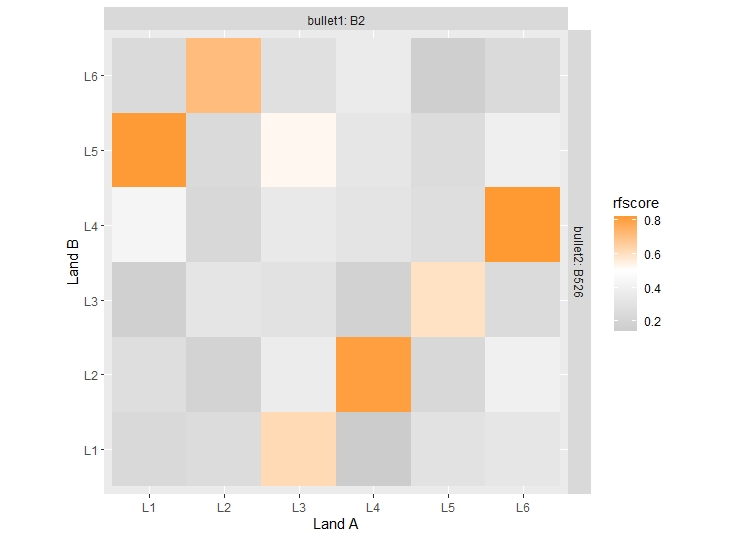
\includegraphics[width=\linewidth]{images/Test_Fire_F526} \caption{Diagonal correspondence (in orange) among lands indicate a match, as shown here. Image generated from Houston dataset by authors.}\label{fig:grid}
\end{figure}

This algorithm was trained on Hamby's Consecutively Rifled Ruger Barrel Study data sets 252 and 173 (Vanderplas et al., 2020), and the final random forest was able to correctly predict all matches and non-matches (Hare et al., 2017, p. 2350).
Three sets were then used to verify the algorithm: Hamby set 44, Phoenix PD, and Houston FSC (Vanderplas et al., 2020, p. 5).
The algorithm performed well for undamaged bullets, and was able to completely distinguish between matches and non-matches when a cutoff value was individually chosen for each data set (Vanderplas et al., 2020, p. 10).

\hypertarget{explainable-machine-learning---previous-research}{%
\subsection{Explainable Machine Learning - Previous Research}\label{explainable-machine-learning---previous-research}}

Jurors' ability to interpret statistical methods and language is \authorcol{in doubt}; in a study conducted by Koehler (2001) with regards to the probability of a random match in DNA evidence, they found that jurors had different interpretations when the probability was presented as 1 out of 1,000 versus 0.1 out of 100, where those presented with a decimal number were more likely to view the probability of a random match as smaller.
In another study, B. Garrett et al. (2018) asked jurors to evaluate evidence that used the following FRStat language, typically used in fingerprint analysis: ``The probability of observing this amount of correspondence is approximately {[}XXX{]} times greater when the impressions are made by the same source rather than by different sources'' (language from Defense Forensic Science Center, 2018).
When asked for the likelihood the defendant committed the crime when presented with the above FRStat language, participants did not provide significantly different likelihoods for values ranging from 10 times greater to 100,000 times greater.
This may demonstrate a lack of understanding when jurors are presented with numerical results for statistical evidence.
ENFSI (2016) proposes a verbal scale to supplement likelihood ratios, which may alleviate some of the burden of statistical interpretation from potential jurors.
This scale ranged from weak support, corresponding to a likelihood ratio between 2 and 10, to very strong support, corresponding to a likelihood ratio greater than 10,000 (ENFSI, 2016, p. 64).
When interviewing judges, lawyers, forensic scientists, and forensic researchers, Swofford \& Champod (2022) found that many expressed concern regarding the interpretation of probabilistic language, and several suggested a combination of both match and probabilistic language.
Hare et al. (2017)'s algorithm differs from previous presentation methods in that its output is a match score, as opposed to a likelihood ratio.
In this study, potential jurors may encounter both the algorithm's match score alongside the categorical match language of the examiner.

\hypertarget{demonstrative-evidence-1}{%
\subsection{Demonstrative Evidence}\label{demonstrative-evidence-1}}

Images are often used to assist individuals in understanding non-image information.
However, images may have an effect of making a scenario more believable, as demonstrated in a study by Cardwell et al. (2016) which involved ``giving'' or ``taking'' food from animals with or without images.
Images are also mentioned as a factor that can influence how truthful individuals view statements in the courtroom - even if no new information is presented through the presence of the image (Kellermann, 2013).
Therefore, the use of images in a courtroom should be studied for an effect with regards to how subjects perceive the evidence presented - namely, if there is a difference in how reliable or credible they feel the experts are, based on the presence or absence of images.
\authorcol{Because the images are intended to aid only in interpretation, we would hope for an increase in understanding across all other conditions, while reliability and credibilty stay the same.}
\authorcol{However, based on previous research, it seems probable that the presence of images would increase the perceived reliability and credibility of the evidence and expert, respectively.}

\hypertarget{methods}{%
\section{Methods}\label{methods}}

\hypertarget{study-format}{%
\subsection{Study Format}\label{study-format}}

\authorcol{First,} participants are presented with a short scenario based on B. Garrett, Scurich, \& Crozier (2020): a bullet is the only evidence recovered from an attempted convenience store robbery, and is tested against a gun found in Richard Cole's car in a routine traffic stop.
\authorcol{Participants are informed that the store clerk was unable to identify the robber because they were wearing a ski mask, and that the testimony presented represented all relevant information.}
\authorcol{They were also advised that they would be unable to re-read testimony, and a notepad was provided for their convenience.}
Participants are then asked to read a transcript of mock court testimony, and rate their impression of the evidence presented, as well as their impression of the experts.
This document included expert testimony, cross examination, and questions from the jury conveyed through the judge regarding error rates.
\authorcol{The expert testified to their qualificiations, as well as the process of bullet matching.}
\authorcol{They then described comparing the fired evidence to a test fire from the defendant's gun, and the results of the comparison.}
\authorcol{When the algorithm was included, the firearms examiner also described the algorithm's match score resulting from this comparison.}
\authorcol{Cross examination included questions regarding the ability to uniquely identify the source of the bullet, as well as the subjectivity of the comparison.}

\authorcol{When the algorithm was included, an algorithm expert then testified.}
\authorcol{They also listed their qualifications and involvement in the development of the algorithm.}
\authorcol{The expert would then describe the process for obtaining a match score (similar to the algorithm description in the previous section).}
\authorcol{They also spoke to the publication history of the algorithm, the code availability, and the algorithm's applicability to the type of firearm considered in the case.}
\authorcol{Cross examination included questions on the newness of the algorithm, as well as subjective aspects of calibration, and limitations with respect to the types of bullets that it can evaluate.}

The testimony was based on actual court testimony provided by forensics experts lawyers, and judges, shown in Appendix \ref{testimony-transcripts}.

\authorcol{After reading the transcript, participants were directed to respond to some questions regarding the testimony.
These questions were largely based on} B. Garrett et al. (2020).
\authorcol{They were first given information about their responsibility as jurors to choose whether or not to convict, and the 'beyond reasonable doubt' threshold was established before asking participants for their conviction decision.}
\authorcol{Participants were also asked to estimate the probability that the defendant committed the crime, and the probability that the gun was involved in the crime.}
\authorcol{These questions were followed by several Likert scales on the strength of evidence, the credibility of the examiners, reliability and scientificity of the evidence, and understanding of the procedures.}
Two attention check questions were asked, in order to ensure that participants were reading both the testimony and the subsequent questions.
The first attention check asked participants to identify the caliber of bullet recovered from the crime scene, while the second attention check asked participants to select a specific value from a Likert scale.

The study includes three \authorcol{independent} variables: \authorcol{presence or absence} of the algorithm, \authorcol{presence or absence} of demonstrative evidence (images), and conclusion (match, exclusion, or inconclusive).
In the case of the algorithm, two testimonies were presented: that of the firearms expert (Terry Smith), and that of the algorithm expert (Adrian Jones).
The firearms expert presented the algorithm results for the case alongside their own analysis, and suggests that the algorithm's results supports their conclusion.
By presenting the algorithm results with the interpretation suggested by the firearms expert, we hoped that potential jurors could use the firearms expert's explanation and conclusion to guide their understanding of the algorithm's results.
The algorithm expert then describes in greater detail the algorithm's process, and its validity for this particular case.
When demonstrative evidence is present, images of rifling (baku13, 2005; Gremi-ch, 2009), a bullet comparison, and algorithm images (such as those shown above) were included alongside the testimony.
In terms of the conclusion: a ``match'' indicated agreement in individual and class characteristics; an ``exclusion'' indicated an agreement of class characteristics, but disagreement in individual characteristics; and an ``inconclusive'' indicated an agreement in class characteristics, but not enough agreement in individual characteristics to state that there was a match.

The number of survey questions that respondents received depended on the scenario; participants who received the algorithm were asked more questions than those who did not receive the algorithm.
For example, participants who did not receive the algorithm were asked about the reliability of the forensics examiner's bullet comparison and the reliability of the field of firearms as a whole.
Those who received the algorithm were asked about the reliability of the forensics examiner's bullet comparison, the reliability of the algorithm's comparison, the overall reliability in the case (which includes both the algorithm comparison and the forensics expert's comparison), as well as the reliability of the field of firearms as a whole.
This same format was used when asking participants about credibility and scientificity.

\hypertarget{prolific}{%
\subsection{Prolific}\label{prolific}}

Participants were recruited using Prolific, an online survey-taking website.
\authorcol{From the Prolific website, participants were directed to a link containing our survey, created using RShiny.}
We selected options to recruit a representative sample of individuals located in the United States, and asked that participants self-screen for jury eligibility before completing the survey.
Jury eligibility was defined as US citizens over the age of majority in their state who had not been convicted of a felony, were not active law enforcement, military, emergency response, or a judge, and who did not have a disability that would prevent them from serving on a jury.
They were also required to have normal or corrected to normal vision, due to the images used in the study.
Participants were compensated with \$8.40 for completing the study, for an hourly compensation rate of about \$27.79 (median completion time of approximately 18 minutes).\\
Individuals who did not include their Prolific identification number and an individual whose notes indicated that they had progressed far enough into the survey to get a separate scenario before restarting were excluded from analysis.

\begin{figure}

{\centering 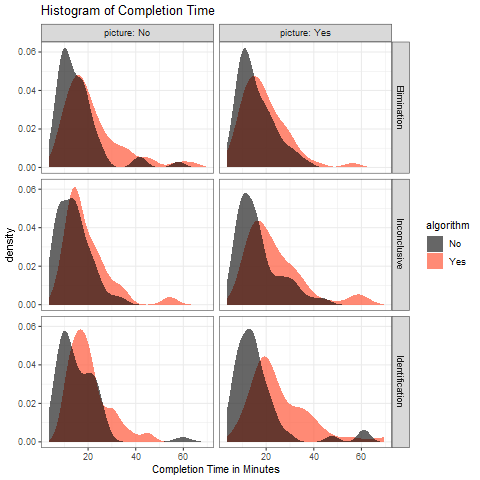
\includegraphics[width=\linewidth]{images/completiontime} 

}

\caption{Completion Time by Condition for all unique fingerprints}\label{fig:completiontime}
\end{figure}

Figure \ref{fig:completiontime} depicts completion times (from completion of the demographics information to the end of the survey) by conditions for unique fingerprints (n=559), excluding 5 observations greater than 75 minutes. In general, it appears that those who received the algorithm condition took slightly more time on average than those who did not (median values of 19.134 minutes and 13.716 minutes, respectively). This is unsurprising, given the increased length of the algorithm condition.

\hypertarget{results}{%
\section{Results}\label{results}}

\authorcol{Due to scale compression, no statistical analysis was performed on this data.}

\hypertarget{participants}{%
\subsection{Participants}\label{participants}}

\begin{figure}

{\centering 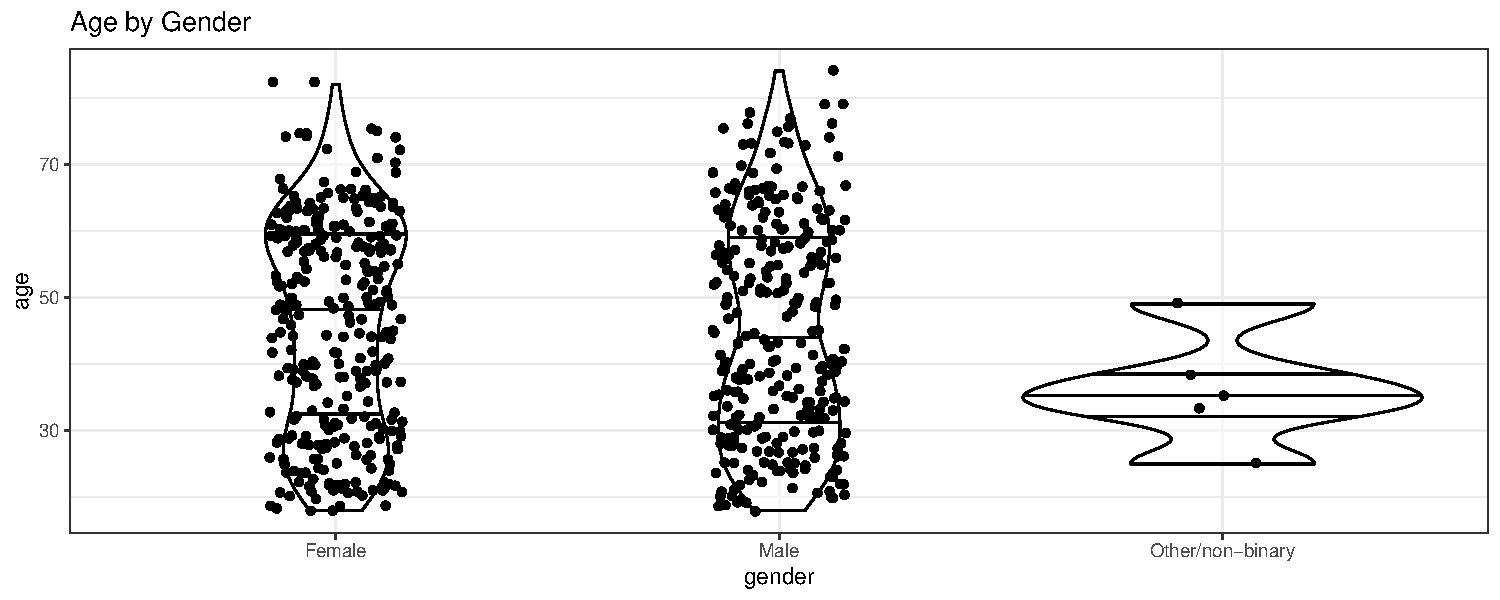
\includegraphics[width=\linewidth]{thesis_files/figure-latex/demographics-1} 

}

\caption{Demographic Information}\label{fig:demographics}
\end{figure}

Of the 636 participants with Prolific ID's who started the survey, there were 324 female participants, 307 male participants, and 5 non-binary participants.
\authorcol{These participants are a representative sample (in terms of age, sex and ethnicity, based on census data) of Prolific participants who are located in the United States.}
The median age was 45.
Age and gender are shown in Figure \ref{fig:demographics}.
An age of 0.2 was excluded due to implausibility and lack of study completion.
591 participants eligible for analysis completed the survey, and 569 participants correctly answered both attention check questions.
\authorcol{In two instances, participants reported being removed from the survey website prior to survey completion, which may have happened in other cases where the participants did not complete the survey.}
The division of correct answers on the attention check questions are shown in Table \ref{tab:attentioncheck}.
These 569 participants were considered for the following analysis.

\begin{table}

\caption{\label{tab:attentioncheck}Attention Check Information}
\centering
\begin{tabular}[t]{l|r|r}
\hline
  & Reading Correct & Reading Incorrect\\
\hline
Caliber Correct & 569 & 12\\
\hline
Caliber Incorrect & 10 & 0\\
\hline
\end{tabular}
\end{table}

\hypertarget{overview}{%
\subsection{Overview}\label{overview}}

Participants were asked a variety of questions in order to assess their thoughts and feelings on the case and the evidence presented.
Two questions related to probability: respondents were asked to provide a value for the probability that the gun was at the crime scene, and to provide a value for the probability that Richard Cole (the defendant) committed the crime.
Another question asked participants if they would convict Cole, based on the evidence.
Questions of credibility, reliability, and scientificity were assessed using a 7-point Likert scale (eg. ``Extremely unscientific'' to ``Extremely scientific'').
Understanding was ranked on a 5-point Likert scale (``I understood nothing'' to ``I understood everything'').
Participants were also asked about uniqueness of firearm toolmarks, as a simple yes/no question.
Strength of evidence was ranked on a 9-point Likert scale (``Not at all strong'' to ``Extremely strong''). The perceived frequency with which firearms examiners made mistakes was assessed on a 7-point Likert scale (``Never'' to ``Always'').

\hypertarget{probability}{%
\subsection{Probability}\label{probability}}

There is a difference in the perceived probability that Cole committed the crime as well as the perceived probability that the gun was present at the crime scene based on the examiner's decision, as shown in Figure \ref{fig:probalgorithm}.
The match condition resulted in high probabilities, while the non-match condition resulted in low probabilities, indicating that participants reacted to the examiner's testimony.
A wider range of probability values were observed for the inconclusive decision, without the high peaks that were present for conclusive decisions.
Definite conclusions of match or not a match resulted in higher peaks at more extreme values for the probability that the gun was at the crime scene, compared with the probability that Cole committed the crime.
This may indicate that some individuals are distinguishing between evidence that the weapon was used and evidence against Cole.
The inconclusive decision resulted in a more spread out distribution that is practically the same for both the probability that the gun was at the crime scene and the probability that Cole committed the crime, with participants generally selecting values below 50\%.

For both Cole and the gun, values are slightly more concentrated toward the lower end of the scale when the algorithm is absent for the non-match condition, and the inconclusive decision produced similar densities across both algorithm conditions.
In the case of the gun's involvement, values are more concentrated toward the higher end of the scale when the algorithm is present for the match condition.
There is no real difference between match distributions for the probability that Cole committed the crime.
The vertical lines indicate the match score presented by the algorithm (0.034 or 3.4\% for the non-match condition, 0.34 or 34\% for the inconclusive condition, and 0.989 or 98.9\% for the match condition).
These are displayed in order to visually assess whether the subjects are anchoring to the given match score when assessing the probability of the gun being present at the crime scene.
Because the match score is on a scale of 0 to 1, this value could be misinterpreted as a probability for the gun being used in the crime.
It does not appear that the participants are anchoring to this value, however, as the distributions do not correspond more to the line when the algorithm is present.

\begin{figure}

{\centering 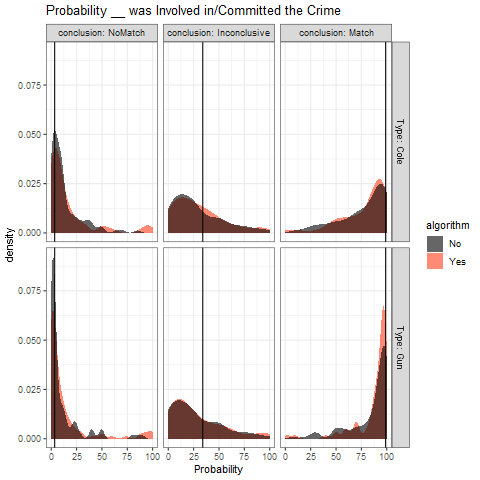
\includegraphics[width=\linewidth]{images/probalgorithm} 

}

\caption{Probability the gun was used in the crime, or that Cole committed the crime. Black lines indicate bullet match scores for the algorithm.}\label{fig:probalgorithm}
\end{figure}

\hypertarget{probability-and-guilt}{%
\subsubsection{Probability and Guilt}\label{probability-and-guilt}}

After reading the testimony, the participants were given the following question:
``The State has the burden of proving beyond a reasonable doubt that the defendant is the person who committed the alleged crime.
If you are not convinced beyond a reasonable doubt that the defendant is the person who committed the alleged crime, you must find the defendant not guilty.
Would you convict this defendant, based on the evidence that you have heard?''
10 out of 196 individuals in the non-match category, 13 out of 191 individuals in the inconclusive category, and 112 out of 182 individuals in the match category chose to convict, despite the bullet matching being the only evidence against Cole in the crime.
As \ref{fig:probguilt} illustrates, across all categories individuals who chose to convict generally assigned a higher probability to Cole committing the crime than those who did not choose to convict.
The same general trend of higher probability values for those who chose to convict and lower probability values for those who chose not to convict is also seen for non-match and inconclusive conditions when discussing the probability that the gun was used in the crime.
However, in the case of the match condition, those who did not convict gave a generally higher probability that the gun was used in the crime than the probability that Cole committed the crime, resulting in comparable values (albeit with more variability) to those who chose to convict.

\begin{figure}

{\centering 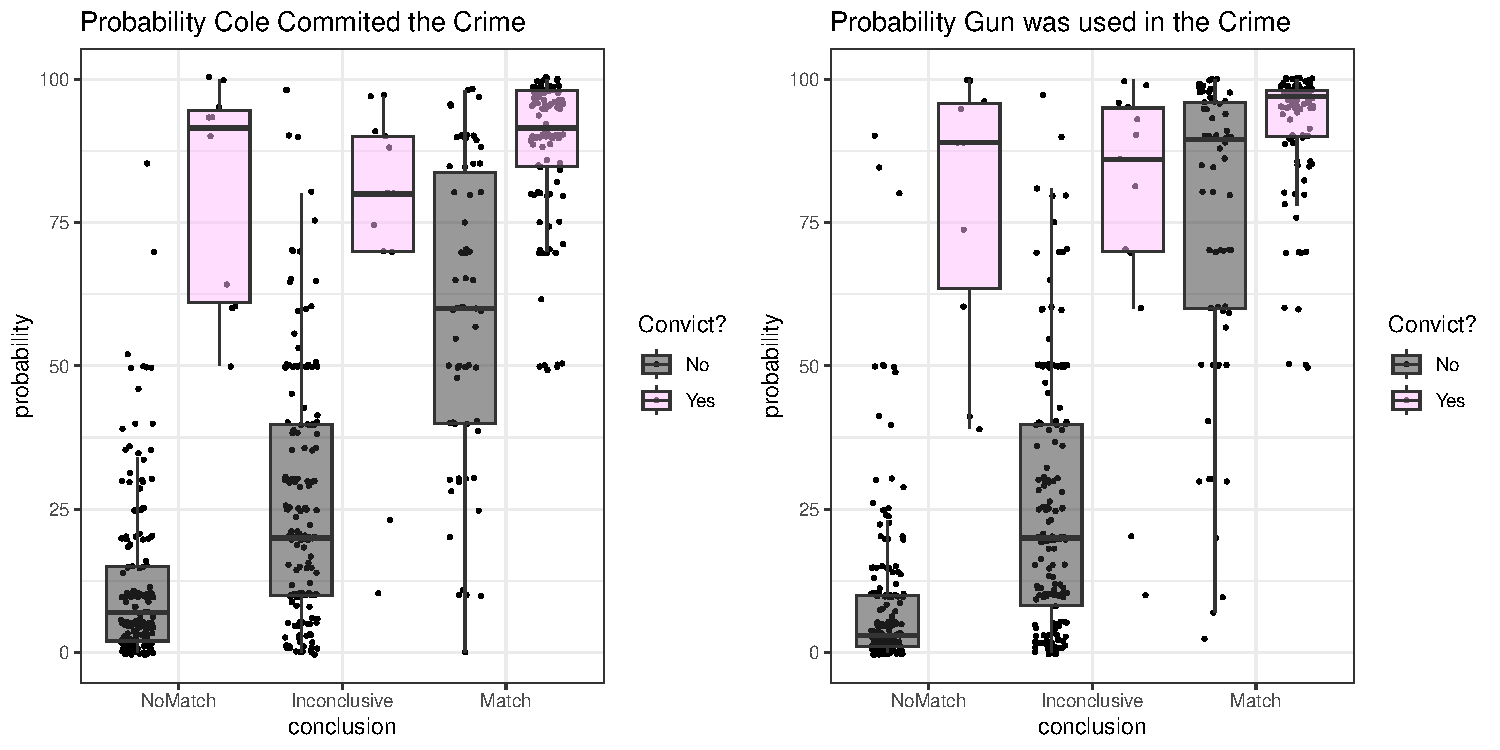
\includegraphics[width=\linewidth]{thesis_files/figure-latex/probguilt-1} 

}

\caption{Probabilities based on whether the participants thought the defendant was guilty}\label{fig:probguilt}
\end{figure}

\hypertarget{credibility}{%
\subsection{Credibility}\label{credibility}}

Through all conditions, the level of credibility remained approximately the same for both the firearms examiner and the algorithm expert.
As Figure \ref{fig:cred} demonstrates, ``Extremely credible'' was by far the most selected category for the firearms examiner, with some people selecting ``Moderately credible'', while the other categories quickly drop off in responses.
This trend was also reflected in the data for the algorithm expert, and can be seen in most histograms resulting from this study (leading to a question of scale compression).
The lack of difference based on examiner decision, image, or algorithm (in the case of the firearms examiner) provides a hopeful indication that the credibility of expert witnesses is not necessarily swayed by the facts of the case or the presence of images, when their written testimony remains the same.

\begin{figure}

{\centering 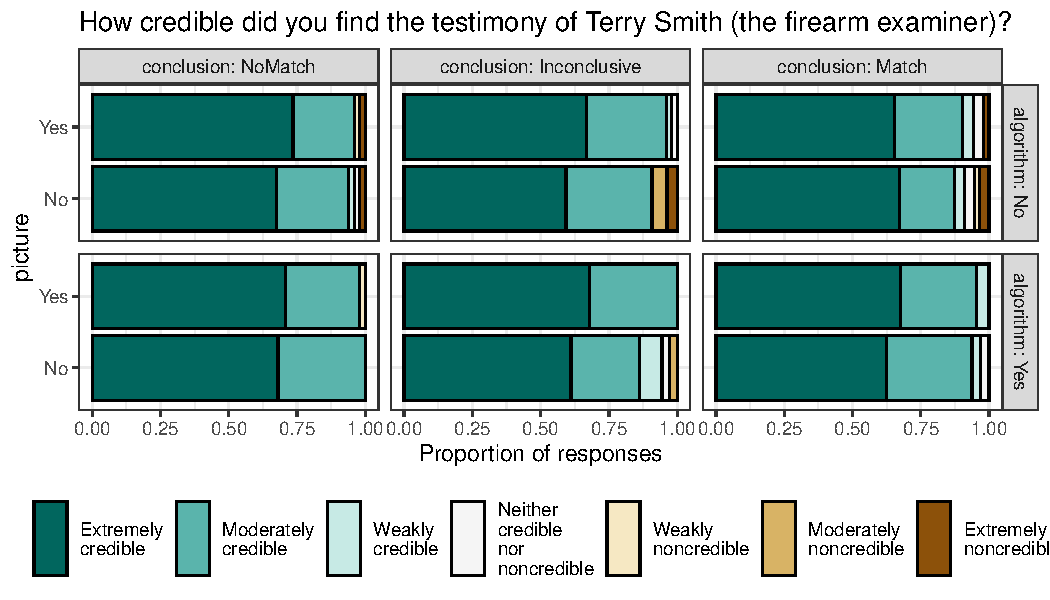
\includegraphics[width=\linewidth]{thesis_files/figure-latex/cred-1} 

}

\caption{Histogram of Firearms Examiner Credibility}\label{fig:cred}
\end{figure}

\hypertarget{reliability}{%
\subsection{Reliability}\label{reliability}}

In terms of reliability, participants appeared to find the case evidence less reliable when an inconclusive decision was given than they did when a conclusive decision was reached, as shown in Figure \ref{fig:caserel}.
Note that this question was only answered by participants who received the algorithm condition and is meant to encompass both the examiner's comparison and the algorithm comparison.
As with the credibility condition, the majority of individuals selected the two highest conditions, ``Moderately reliable'' and ``Extremely reliable'', across all categories of conclusions.
In the case of an inconclusive decision, the highest proportion of participants selected ``Moderately reliable'', while for the conclusive decisions, the highest proportion of participants selected ``Extremely reliable''.

\begin{figure}

{\centering 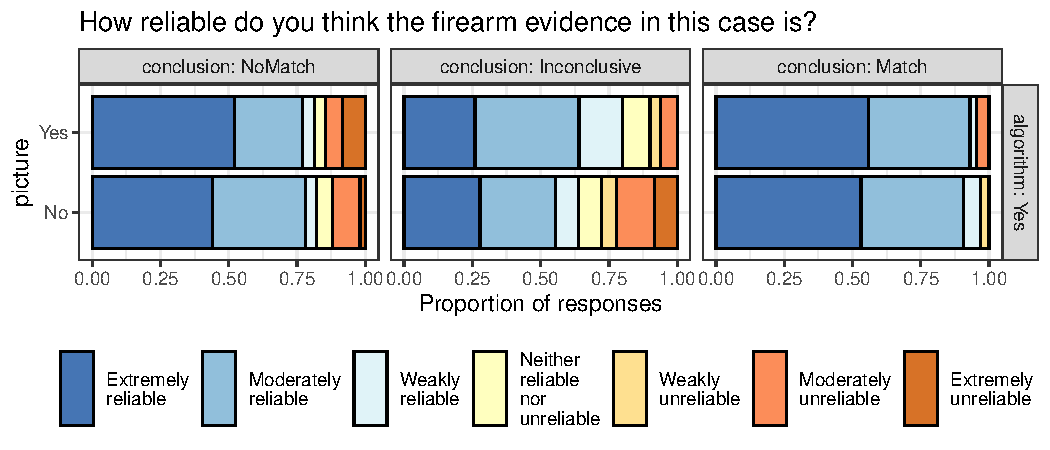
\includegraphics[width=\linewidth]{thesis_files/figure-latex/caserel-1} 

}

\caption{Histogram of overall case reliability}\label{fig:caserel}
\end{figure}

Individuals were also asked to rate the general reliability of firearms evidence as a field (Figure \ref{fig:genrel}).
As with case reliability, those who received an inconclusive condition were more likely to select ``Moderately reliable'' than they were to select ``Extremely reliable''.
This trend is also shown in the non-match condition when the algorithm is present.
However, it is not reflected in the match condition.
When the algorithm is absent, both the match and the non-match conditions appear to produce approximately equal proportions for the two highest categories of reliability.
As with previous responses, all other categories are sparsely populated.

\begin{figure}

{\centering 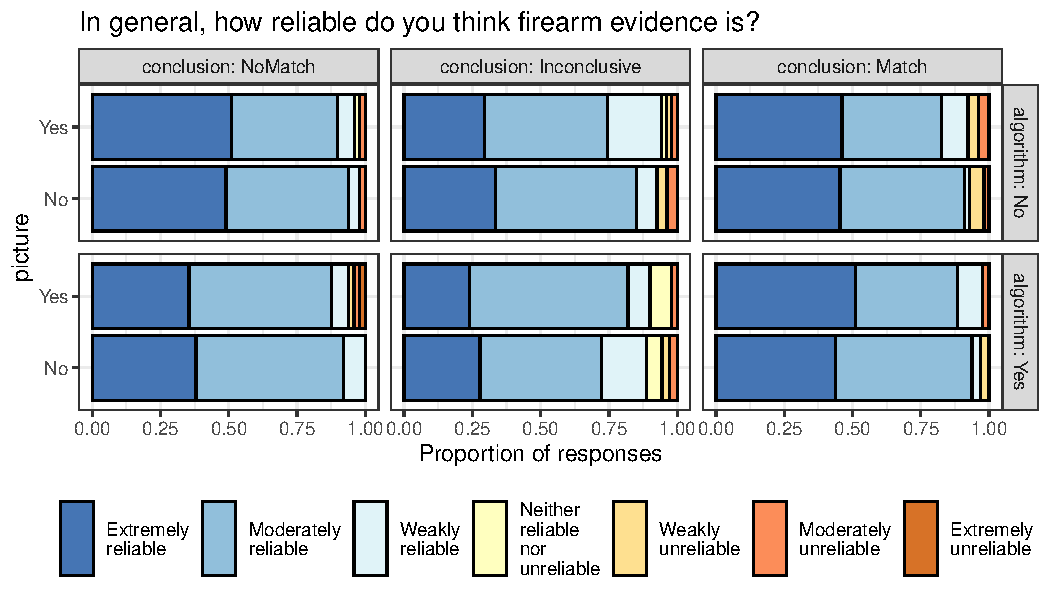
\includegraphics[width=\linewidth]{thesis_files/figure-latex/genrel-1} 

}

\caption{Histogram of perceived firearm reliability as a field}\label{fig:genrel}
\end{figure}

In all conditions, participants were asked to rate the reliability of the examiner's subjective opinion of the firearm evidence (Figure \ref{fig:examrel}).
Participants from both the algorithm and non-algorithm groups gave similar reliability ratings in the non-match condition: most chose ``Moderately reliable'' or ``Extremely reliable'', with more choosing ``Extremely reliable''.
For inconclusive and match conditions, there is a difference in proportions of which category is selected based on the presence or the absence of the algorithm.
When the algorithm is absent, the trend is fairly similar to that in the non-match condition: between the two highest categories, the majority chose ``Extremely reliable''.
However, in the case that the algorithm was present, this trend was flipped: more participants chose ``Moderately reliable'' over ``Extremely reliable''.

\begin{figure}

{\centering 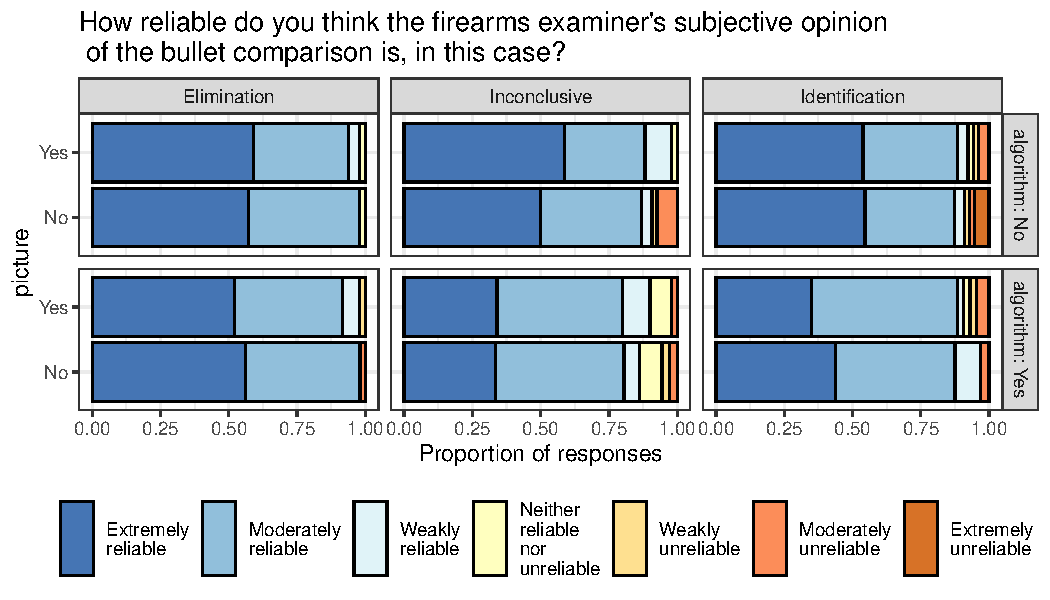
\includegraphics[width=\linewidth]{thesis_files/figure-latex/examrel-1} 

}

\caption{Histogram of perceived firearm exam reliability}\label{fig:examrel}
\end{figure}

Individuals who received the algorithm were also asked to rate algorithm reliability, responses are shown in Figure \ref{fig:algrel}.
The responses were in many ways similar to those given in the case of general reliability: those who received an inconclusive decision were more likely to give a lower reliability rating, and the two highest categories were by far the most selected.
Both also demonstrated a higher selection of ``Weakly reliable'' when individuals were presented with an inconclusive decision.

\begin{figure}

{\centering 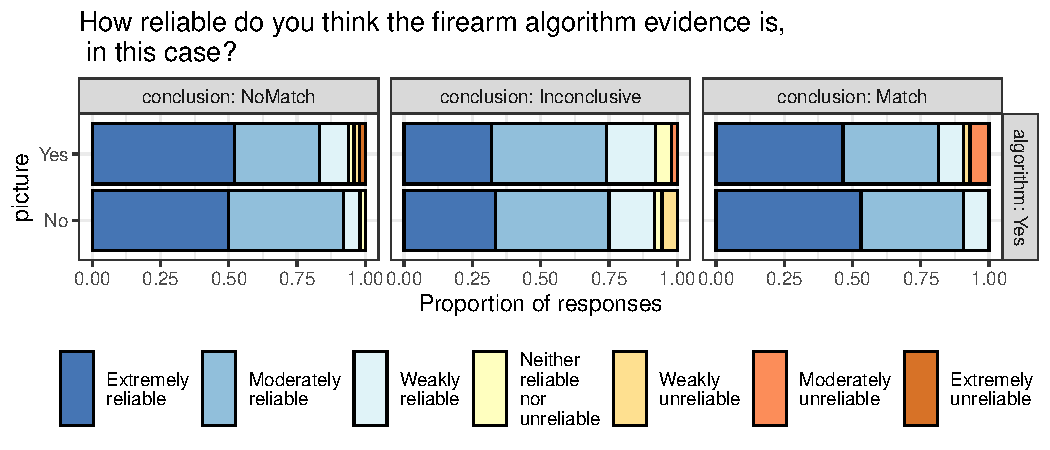
\includegraphics[width=\linewidth]{thesis_files/figure-latex/algrel-1} 

}

\caption{Histogram of perceived algorithm reliability}\label{fig:algrel}
\end{figure}

In most cases, individuals gave lower reliability ratings when an inconclusive decision was reached.
They also tended to select the two highest reliability categories, ``Moderately reliable'' and ``Extremely reliable'', regardless of other conditions.
The presence or absence of images did not have a noticeable effect on reliability ratings.
The presence of the algorithm is related to a slight reduction in reliability ratings for the firearms examiner's personal bullet comparison, in the case of an inconclusive or match decision.

\hypertarget{scientificity}{%
\subsection{Scientificity}\label{scientificity}}

Participants were also asked about how scientific they felt the process was, in a similar four-question format to reliability.
These results bore some similarity in responses to reliability across questions.
As previously stated, images did not appear to have a large effect and the two highest categories were by far the most selected.
When asked about their rating of how scientific the evidence was in the case overall, those receiving the inconclusive condition were less likely to select ``Extremely scientific'' compared to their counterparts given conclusive conditions.

In terms of firearms evidence as a field, results are shown in Figure \ref{fig:gensci}.
Here, as before, those who received the inconclusive decision were more likely to select ``Moderately scientific'' over ``Extremely scientific'' for both cases of the algorithm.
A higher proportion of individuals selected ``Extremely scientific'' for conclusive decisions when the algorithm was present compared to when the algorithm was absent.

\begin{figure}

{\centering 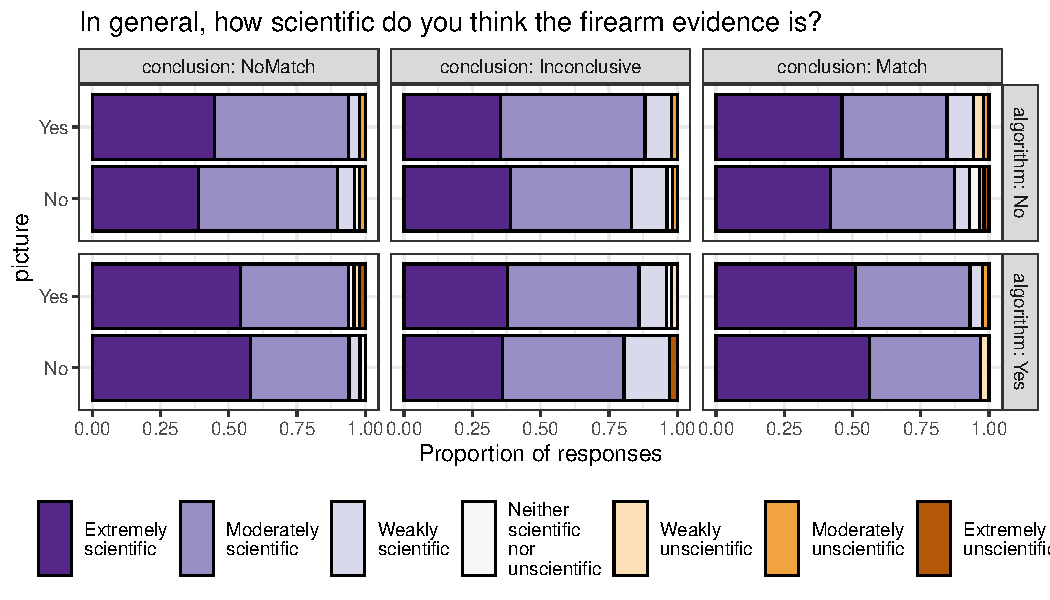
\includegraphics[width=\linewidth]{thesis_files/figure-latex/gensci-1} 

}

\caption{Histogram of perceived firearm scientificity as a field}\label{fig:gensci}
\end{figure}

Regarding how scientific individuals found the examiner's comparison, the algorithm only seemed to have an effect when individuals were presented with an inconclusive decision (\ref{fig:examsci}).
When the algorithm was not present, people were more likely to select ``Extremely scientific'', resulting in a proportion on par with conclusive results.
When the algorithm was present, however, ``Moderately scientific'' became the most popular choice for those who received an inconclusive decision, which reflects the general trend of the majority of participants selecting the second highest category for inconclusive results.
Results for conclusive categories are fairly similar across algorithm conditions, with a close split between ``Moderately scientific'' and ``Extremely scientific''.

\begin{figure}

{\centering 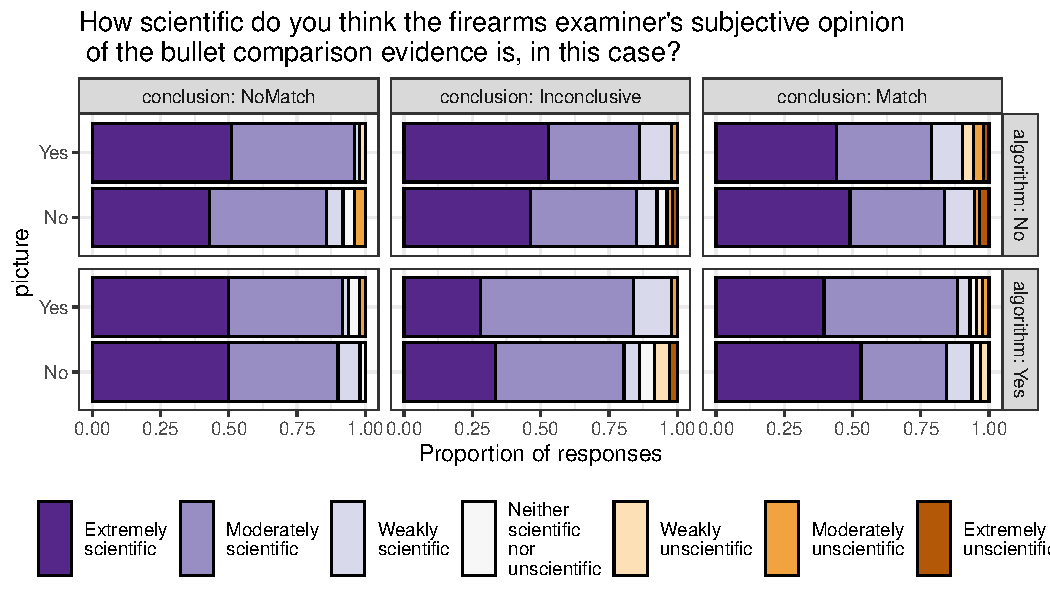
\includegraphics[width=\linewidth]{thesis_files/figure-latex/examsci-1} 

}

\caption{Histogram of perceived scientificity of the bullet comparison of the firearm examiner}\label{fig:examsci}
\end{figure}

Participants gave the algorithm a high rating in scientificity across all categories of conclusions, as shown in Figure \ref{fig:algsci}.
Here, all decisions had the highest proportion of respondents select ``Extremely scientific''.
The proportion selecting ``Moderately scientific'' was noticeably lower than the proportion selecting ``Extremely scientific''.
The use of demonstrative evidence did not have a visible effect.

\begin{figure}

{\centering 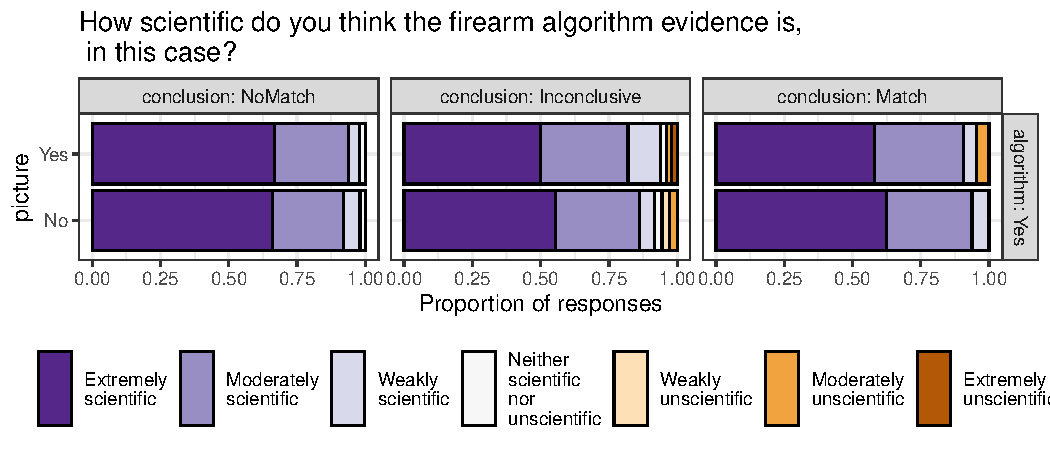
\includegraphics[width=\linewidth]{thesis_files/figure-latex/algsci-1} 

}

\caption{Histogram of perceived algorithm scientificity in this case}\label{fig:algsci}
\end{figure}

In summary, the algorithm is related an an increase of perceived scientificity for the field of firearm evidence as a whole when individuals were presented with a conclusive decision, and ``Extremely scientific'' was the most selected category when evaluating the scientificity of the algorithm evidence regardless of conclusion.
As for how individuals rated the scientificity of the algorithm expert's comparison, the algorithm only appeared to influence results for those who received the inconclusive condition.
Individuals who received the algorithm were more likely to select ``Moderately scientific'', while those who did not receive the algorithm were more likeley to select ``Extremely scientific''.

\hypertarget{understanding}{%
\subsection{Understanding}\label{understanding}}

Individuals were asked to rate their understanding of both the algorithm and the examiner's personal bullet comparison on a 5-point Likert scale. Most responses ranged from 3 (``I understood about half of the method'') to 5 (``I understood everything''), leading to less scale compression than was seen in scales relating to credibility, reliability, and scientificity.

For the firearms examiner's personal comparison, few individuals selected that they understood less than half the method (Figure \ref{fig:expunder}).
Those who did not receive the algorithm were more likely to select ``I understood everything'' compared to those who did receive the algorithm, across all conclusions.
There was not a discernible difference in responses based on the presence or absence of images.

\begin{figure}

{\centering 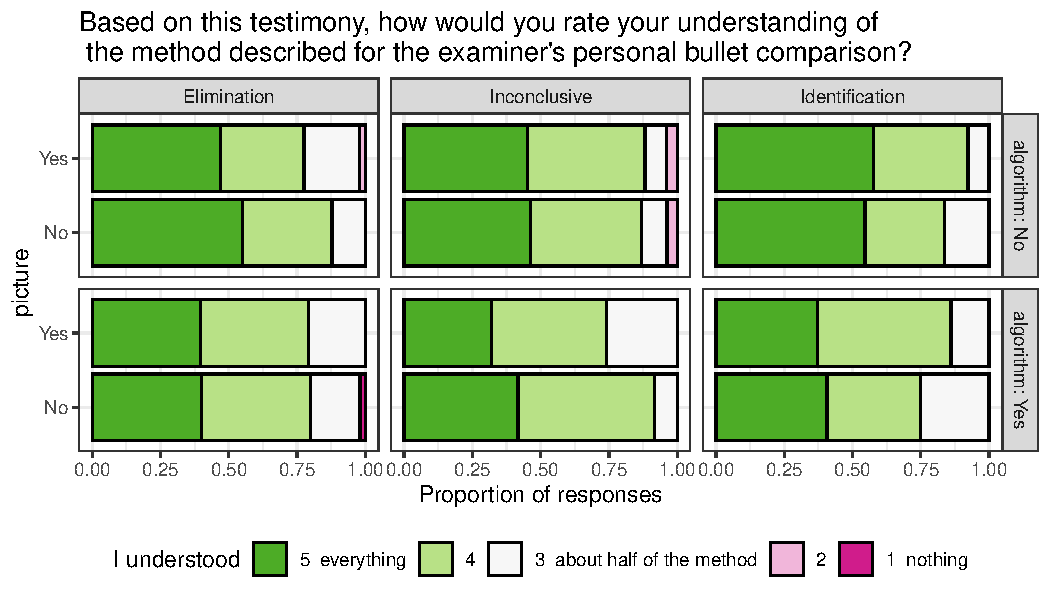
\includegraphics[width=\linewidth]{thesis_files/figure-latex/expunder-1} 

}

\caption{Histogram of understanding for the explanation of the firearms examiner}\label{fig:expunder}
\end{figure}

The results for the particpants' understanding of the algorithm description differs based on the presence or absence of images (Figure \ref{fig:expunder}).
When images are absent, participants selected values from ``I understood about half the method'' to ``I understood everything'' with a fairly uniform frequency, with a few participants selecting values in the lower categories.
When images were present, however, category selection appeared to relate to conclusion.
Those receiving the match condition were more likely to select 4 than other categories, meaning that they felt they understood more than half of the method but didn't understand everything.
Those receiving the non-match condition were more likely to select that they understood half of the method compared to other categories.
Those with an inconclusive condition had responses fairly evenly distributed across the top three categories, similar to when images were absent.
As in the case without images, few individuals indicated that they understood less than half of the method.
It is unclear what may have caused these differences in ratings of understanding.

\authorcol{To investigate this potential relationship further, Table} \ref{tab:undertb}
\authorcol{was created. Because the counts are so small for the individual cells, the resemblence to a relationship based on conclusion is possibly due to random variation.}

\begin{table}

\caption{\label{tab:undertb}Understanding Frequency}
\centering
\begin{tabular}[t]{l|r|r|r}
\hline
  & NoMatch & Inconclusive & Match\\
\hline
2.0 & 1 & 4 & 2\\
\hline
3 <br/> I understood about half of the method & 25 & 16 & 7\\
\hline
4.0 & 14 & 16 & 27\\
\hline
5 <br/> I understood everything & 8 & 14 & 7\\
\hline
\end{tabular}
\end{table}

\hypertarget{uniqueness}{%
\subsection{Uniqueness}\label{uniqueness}}

Individuals were asked whether or not they thought that guns left unique markings on discharged bullets and casings after reviewing the testimony.
Of the 569 responses, only 16 individuals indicated that they did not think guns left unique markings.
These respondents were split across conditions.
Thus, respondents in this study overwhelmingly believe in the uniqueness of markings on discharged bullets.

\hypertarget{strength}{%
\subsection{Strength}\label{strength}}

\begin{figure}

{\centering 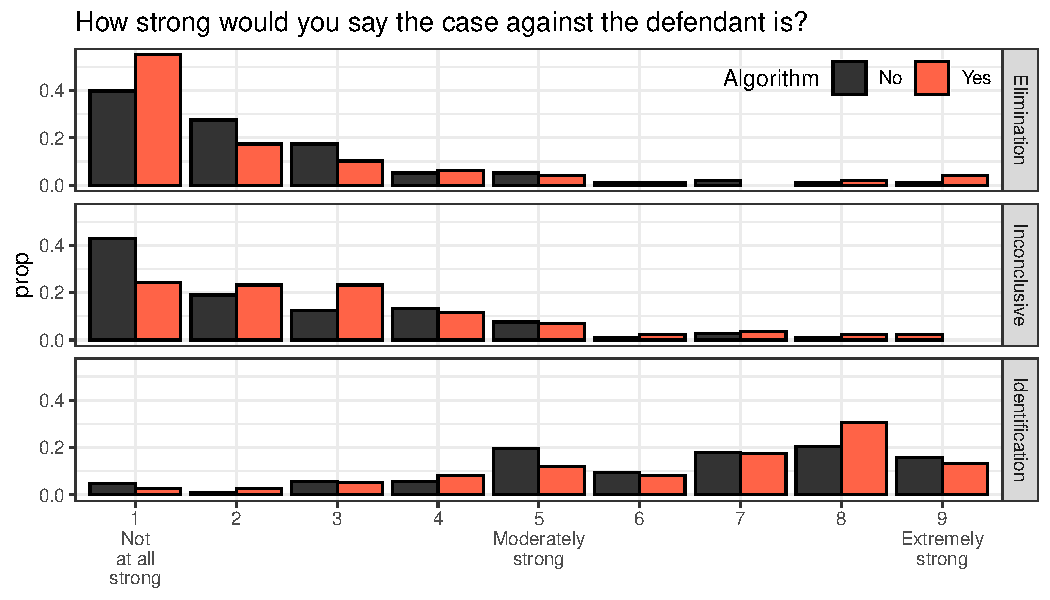
\includegraphics[width=\linewidth]{thesis_files/figure-latex/strength-1} 

}

\caption{Histogram of perceived strength of evidence against the defendant}\label{fig:strength}
\end{figure}

Individuals were also asked to rate the strength of evidence, both against Richard Cole and against the gun.
\authorcol{Unlike questions of reliability, credibility, and scientificity, strength of evidence was measured on a 9-point Likert scale, without worded values for intermittent categories, following the procedure of @garrettMockJurorsEvaluation2020.}

When asked about the case against the defendant, shown in Figure \ref{fig:strength}, there was a small difference in terms of the algorithm.
When the examiner reached a non-match conclusion, individuals who also received the algorithm were more likely to select the lowest category (``not at all strong'') compared to those who did not receive the algorithm.
Alternatively, in the case of an inconclusive decision, individuals who did not receive the algorithm were more likely to select ``not at all strong'' compared to those who did receive the algorithm.
For the match condition, responses were more widely distributed.

\begin{figure}

{\centering 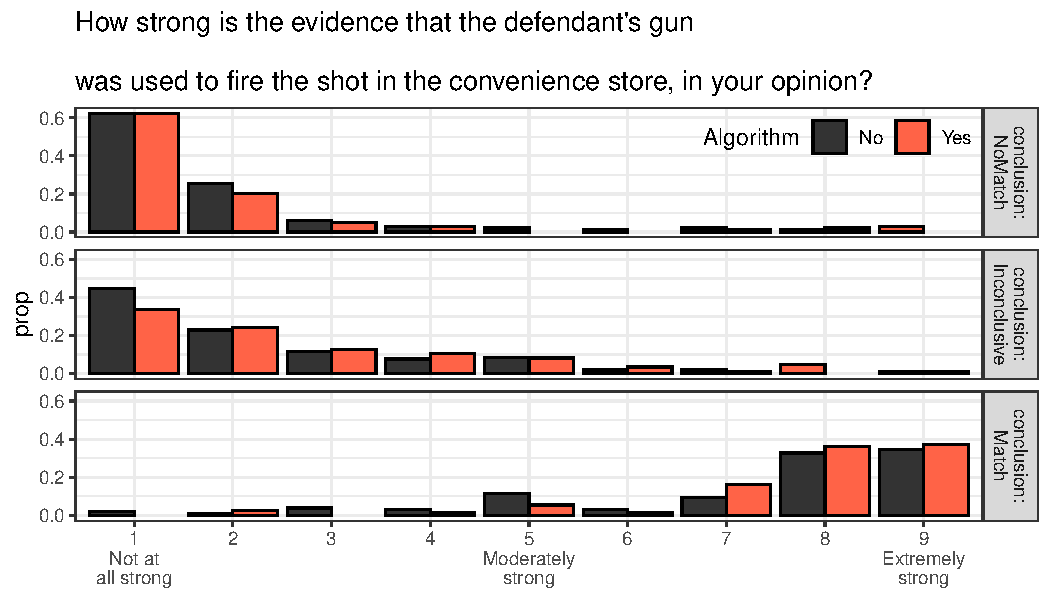
\includegraphics[width=\linewidth]{thesis_files/figure-latex/gunstrength-1} 

}

\caption{Histogram of perceived strength of evidence against the gun}\label{fig:gunstrength}
\end{figure}

When asked about the strength of evidence against the defendant's gun, there was no real difference between those who received the algorithm and those who did not (\ref{fig:gunstrength}).
The match condition resulted in a more concentrated distribution at higher strength values than were seen for the strength of evidence against Cole.

\begin{figure}

{\centering 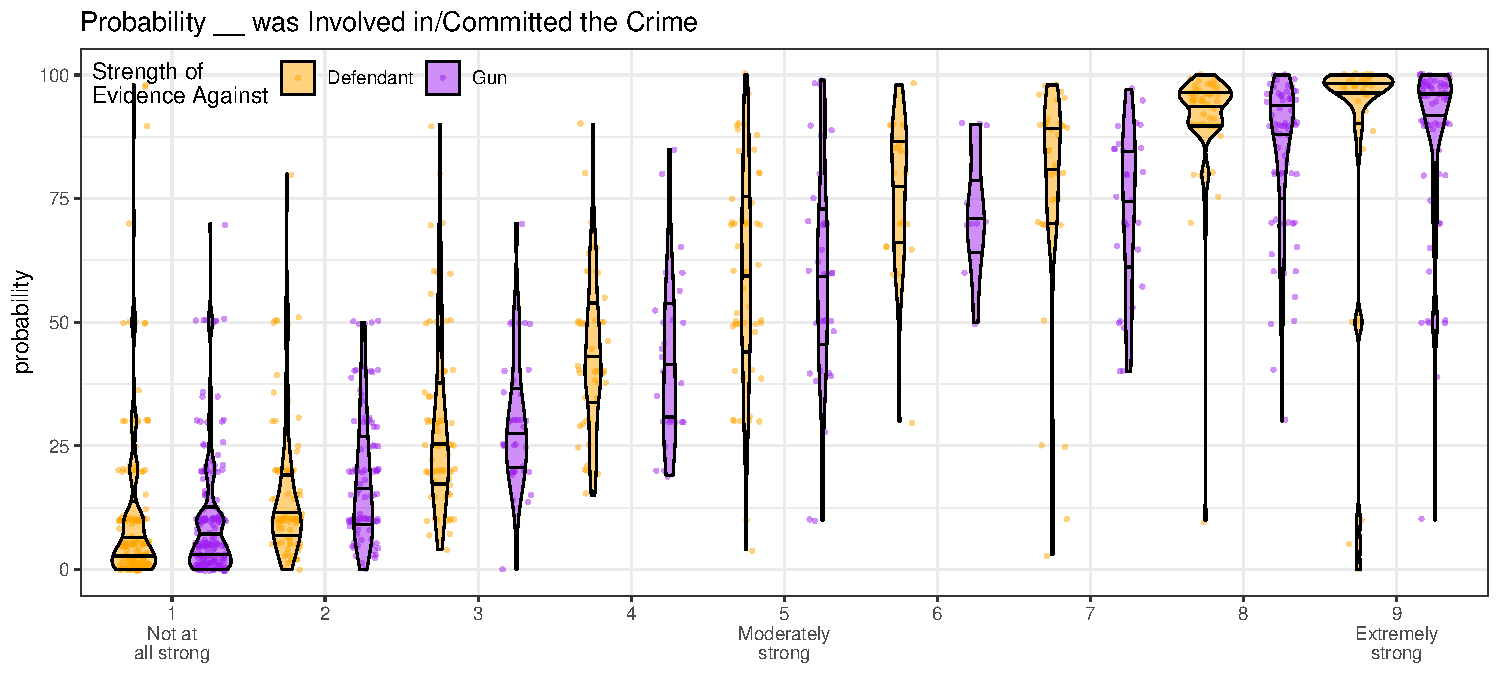
\includegraphics[width=\linewidth]{thesis_files/figure-latex/probstrength-1} 

}

\caption{Probabilities based on perceived strength of evidence.}\label{fig:probstrength}
\end{figure}

In comparing how individuals scored strength of evidence and the probability that they assigned to Cole committing the crime and the gun being present at the crime scene, the results were largely consistent (\ref{fig:probstrength}).
In general, the probability assigned increases as the assigned strength of evidence increases, which is to be expected.

\hypertarget{mistakes}{%
\subsection{Mistakes}\label{mistakes}}

Individuals were asked how often firearms examiners make mistakes when determining whether bullets were fired through the same gun, with a scale from ``Never'' to ``Usually''.
``Rarely'' was by far the most selected category, as shown in Figure \ref{fig:mistakes}.
There does not appear to be a strong relationship between how often individuals felt firearms examiners made mistakes and factors such as conclusion, images, or the algorithm.

\begin{figure}

{\centering 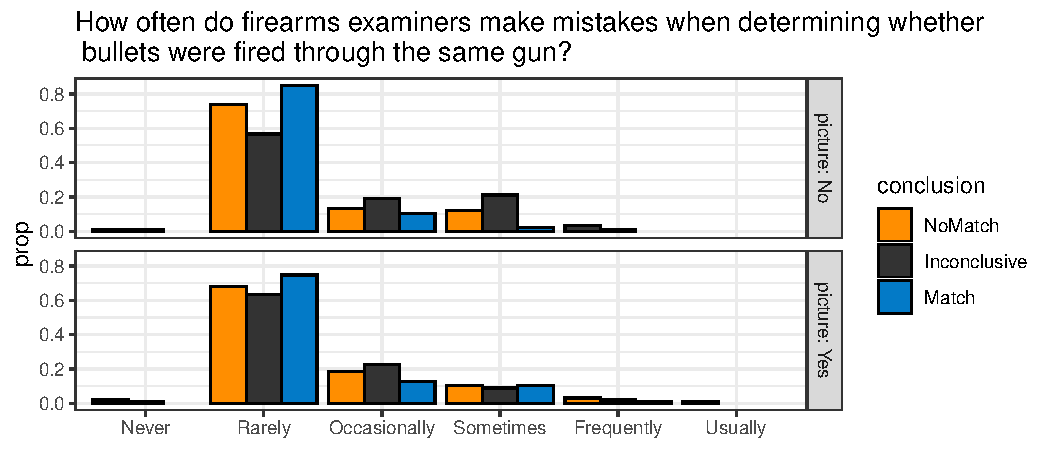
\includegraphics[width=\linewidth]{thesis_files/figure-latex/mistakes-1} 

}

\caption{Histogram of perceived frequency of mistakes made by firearms examiners}\label{fig:mistakes}
\end{figure}

\hypertarget{comparing-algorithm-values-to-examiner-values}{%
\subsection{Comparing Algorithm Values to Examiner Values}\label{comparing-algorithm-values-to-examiner-values}}

Participants who received the algorithm condition were asked to evaluate their feelings on the reliability, credibility, scientificity, and their understanding of both the algorithm method as well as the traditional bullet analysis method, as discussed in previous sections.
Results for both methods were compared on an individual level as well as on a group level.
The group level results are represented in histograms, while the individual level results are represented in parallel coordinates plots.
Note that these results only reflect the feelings of individuals who received the algorithm condition.

\hypertarget{group-level-results}{%
\subsubsection{Group Level Results}\label{group-level-results}}

\begin{figure}

{\centering 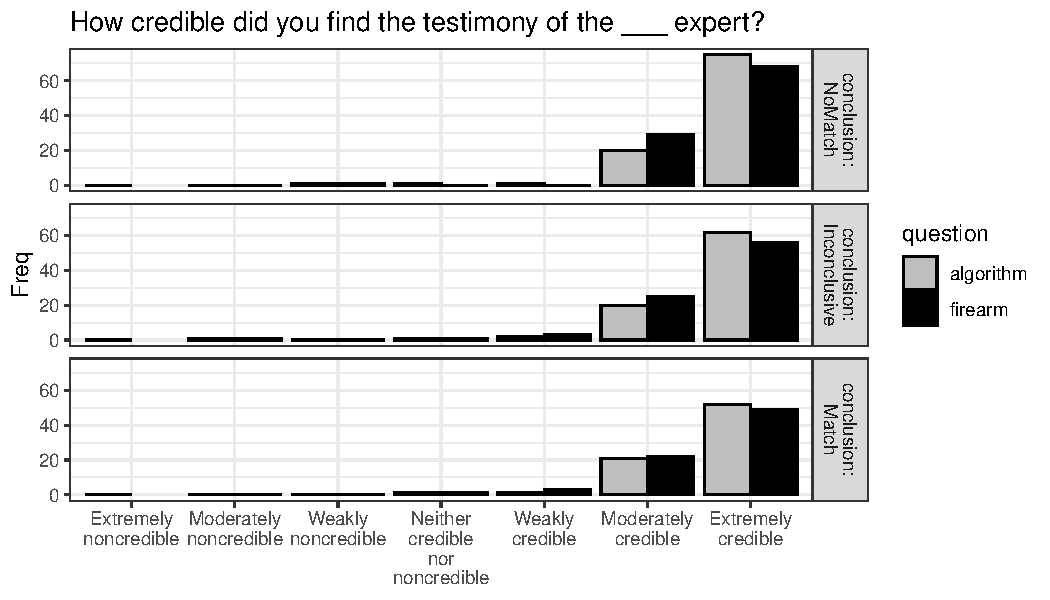
\includegraphics[width=\linewidth]{thesis_files/figure-latex/histcred-1} 

}

\caption{Histogram of perceived credibility of experts}\label{fig:histcred}
\end{figure}

In terms of credibility, as shown in Figure \ref{fig:histcred}, the algorithm and the expert scored fairly similarly, with the algorithm expert resulting in slightly more individuals selecting ``Extremely credible'' than the firearms expert.
As mentioned before, most participants limited their selection to the two highest categories - ``Moderately credible'' and ``Extremely credible''.

\begin{figure}

{\centering 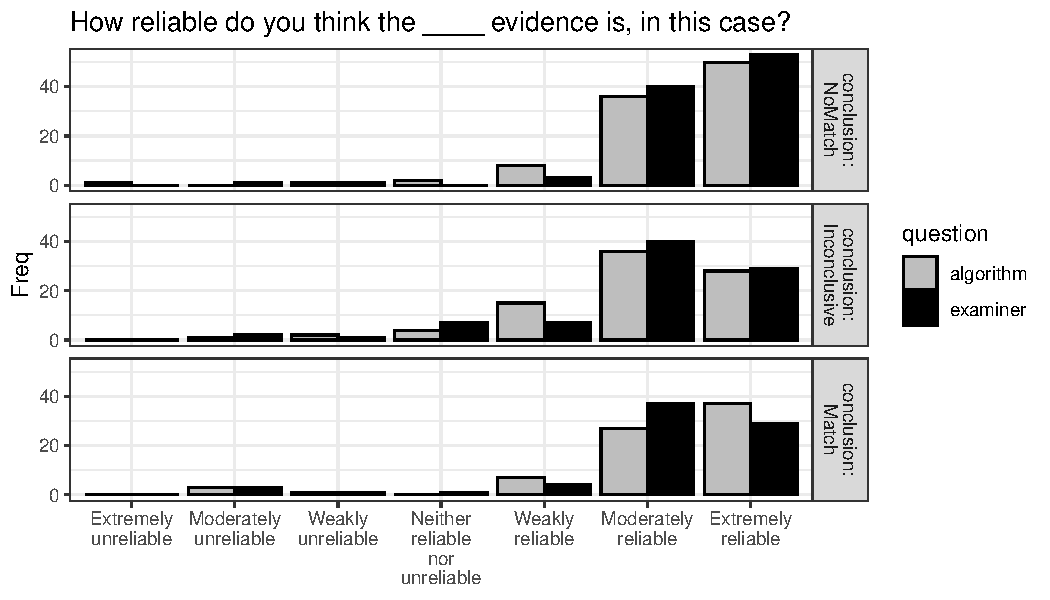
\includegraphics[width=\linewidth]{thesis_files/figure-latex/histrel-1} 

}

\caption{Histogram of perceived reliability of evidence}\label{fig:histrel}
\end{figure}

For reliability, shown in Figure \ref{fig:histrel}, a similar number of individuals selected ``Extremely reliable'' for both the algorithm evidence and the examiner's comparison, with a larger proportion of individuals selecting ``Extremely reliable'' in the match condition when the algorithm is present.
There appears to be, however, a difference in the categories of ``Moderately reliable'' and ``Weakly reliable''.
Individuals were more likely to select that the algorithm was ``Weakly reliable'', while they were less likely to select that the algorithm was ``Moderately reliable'', compared to the examiner.

\begin{figure}

{\centering 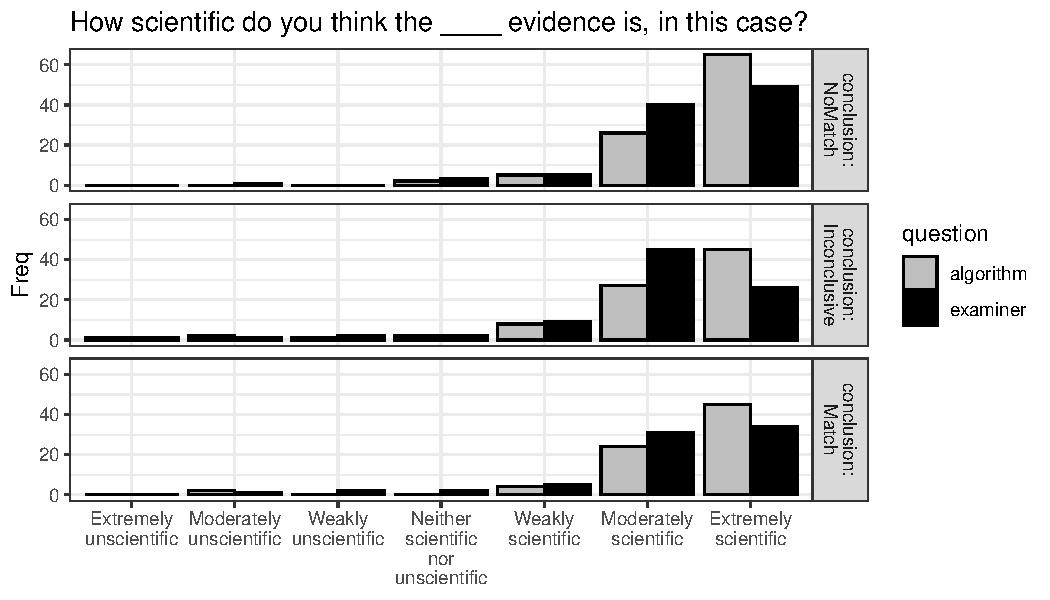
\includegraphics[width=\linewidth]{thesis_files/figure-latex/histsci-1} 

}

\caption{Histogram of perceived scientificity of evidence}\label{fig:histsci}
\end{figure}

Individuals generally saw the algorithm as more scientific than the expert, as shown in Figure \ref{fig:histsci}.
They were more likely to select ``Extremely scientific'' in the case of the algorithm when compared to the expert.
Accordingly, they were less likely to select ``Moderately scientific'' in the case of the algorithm when compared to the examiner.
No real difference can be seen in the lower values on the scale, due to few individuals selecting these categories.

\begin{figure}

{\centering 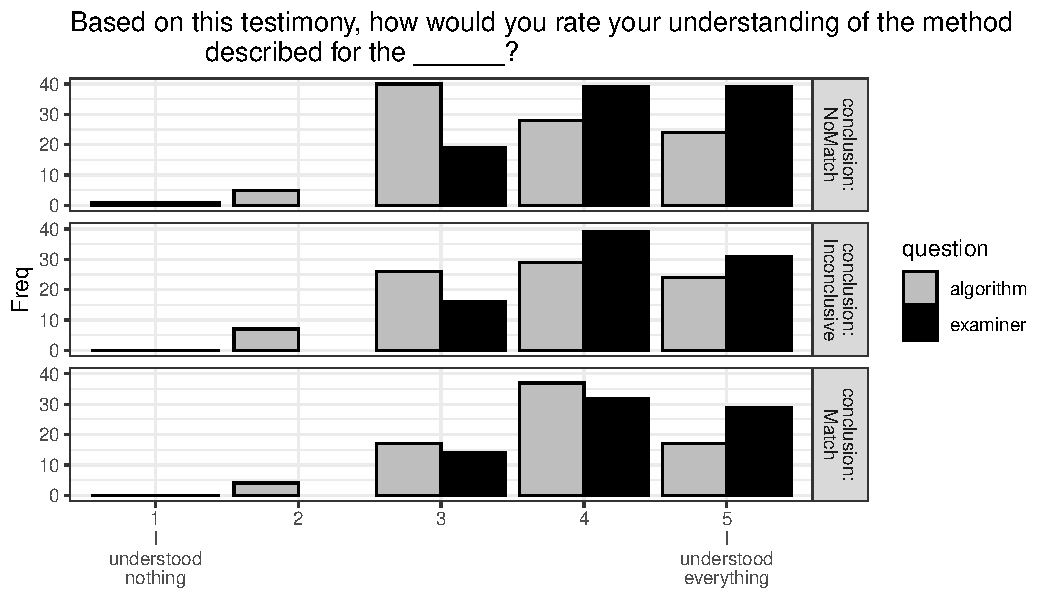
\includegraphics[width=\linewidth]{thesis_files/figure-latex/histunder-1} 

}

\caption{Histogram of participants' understanding}\label{fig:histunder}
\end{figure}

Individuals rated their understanding of the examiner's bullet comparison higher than their understanding of the algorithm method, generally speaking (\ref{fig:histunder}).
Participants were more likely to select a 4 or 5 with regards to their understanding of the examiner's comparison, while they were more likely to select a 3 or 4 with regards to their understanding of the algorithm method.
While these questions gauge how well participants believe they understand the given concepts, Dunning, Heath, \& Suls (2004) indicate that individuals are not unbiased judges of their own understanding.

\hypertarget{individual-level-results}{%
\subsubsection{Individual Level Results}\label{individual-level-results}}

\begin{figure}

{\centering 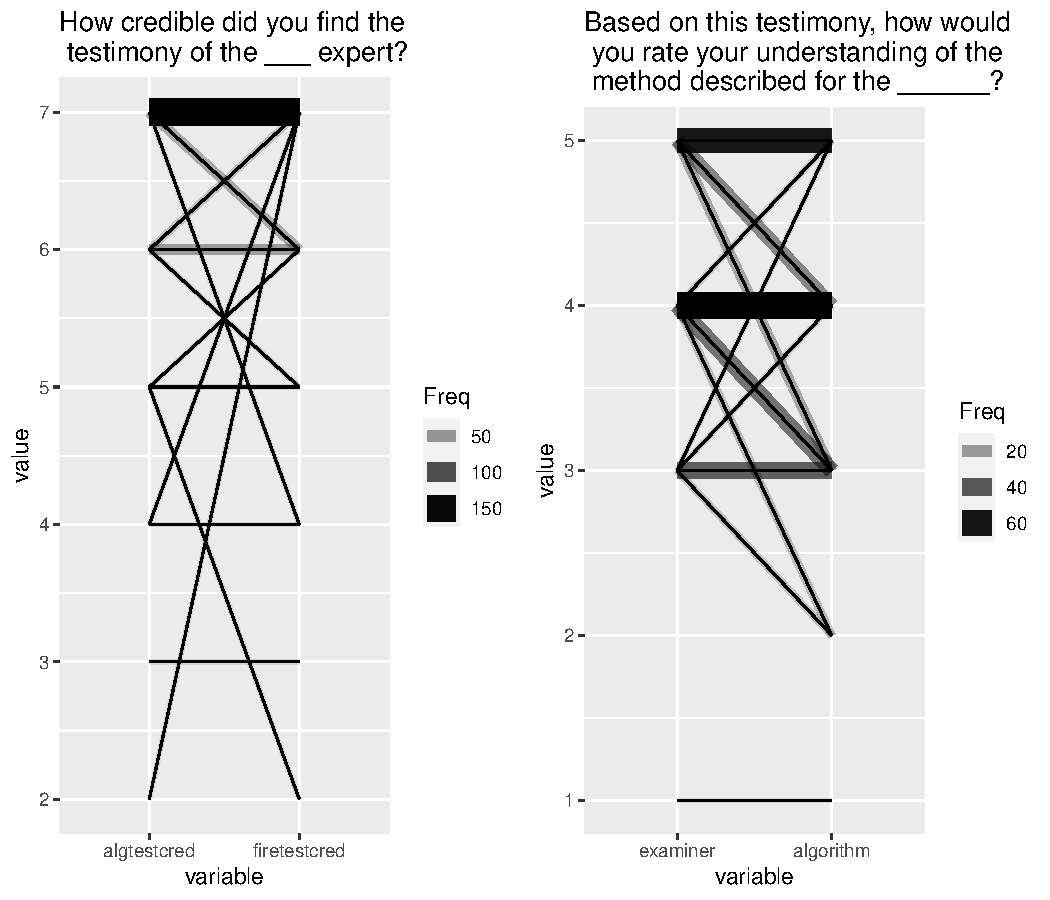
\includegraphics[width=\linewidth]{thesis_files/figure-latex/coordcred-1} 

}

\caption{Plots of understanding and perceived expert credibility}\label{fig:coordcred}
\end{figure}

Figure \ref{fig:coordcred} depicts parallel coordinate plots for participants' ratings of the credibility of the experts, as well as their understanding of the methods described in the testimony.
Higher values indicate higher scores in understanding and credibility. These plots map the frequency that individuals selected the shown combination of values for credibility or understanding.
In the case of credibility, we can see that most individuals selected the highest category of credibility for both the algorithm and the firearms expert.
In the case of understanding, individuals tended to select the two highest categories the most.
It can also be seen that there is a trend of individuals selecting a category lower for the algorithm compared to what they selected for the examiner by the thicker downward line between categories 4 and 5, as well as between categories 4 and 3.
This corresponds to Figure \ref{fig:histunder} in that individuals tend to give higher understanding ratings to the examiner's bullet comparison method than they did for the algorithm.

\begin{figure}

{\centering 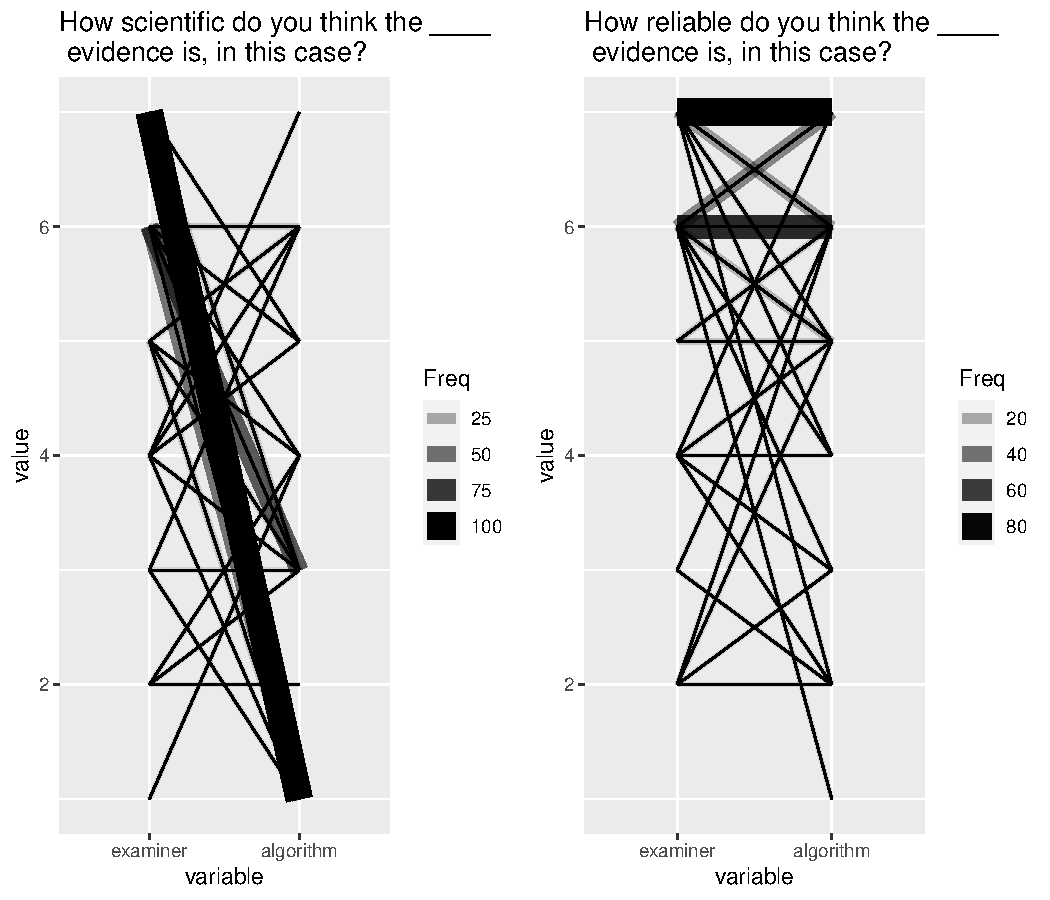
\includegraphics[width=\linewidth]{thesis_files/figure-latex/coordscirel-1} 

}

\caption{Plots of perceived scientificity and reliability of methods}\label{fig:coordscirel}
\end{figure}

Figure \ref{fig:coordscirel} demonstrates the trends for selection for how scientific and reliable individuals felt the evidence was.
In terms of how scientific individuals felt the evidence was, it appears that most participants selected the highest category for both the algorithm and the examiner.
Some participants selected the second highest category for the examiner, and the highest category for the algorithm.
Others selected the second highest category in both cases.
In terms of reliability, participants tended to choose one of the two highest categories for both the algorithm and the examiner.
Some participants switched between the two highest categories for the algorithm or the examiner, in similar numbers.

\begin{figure}
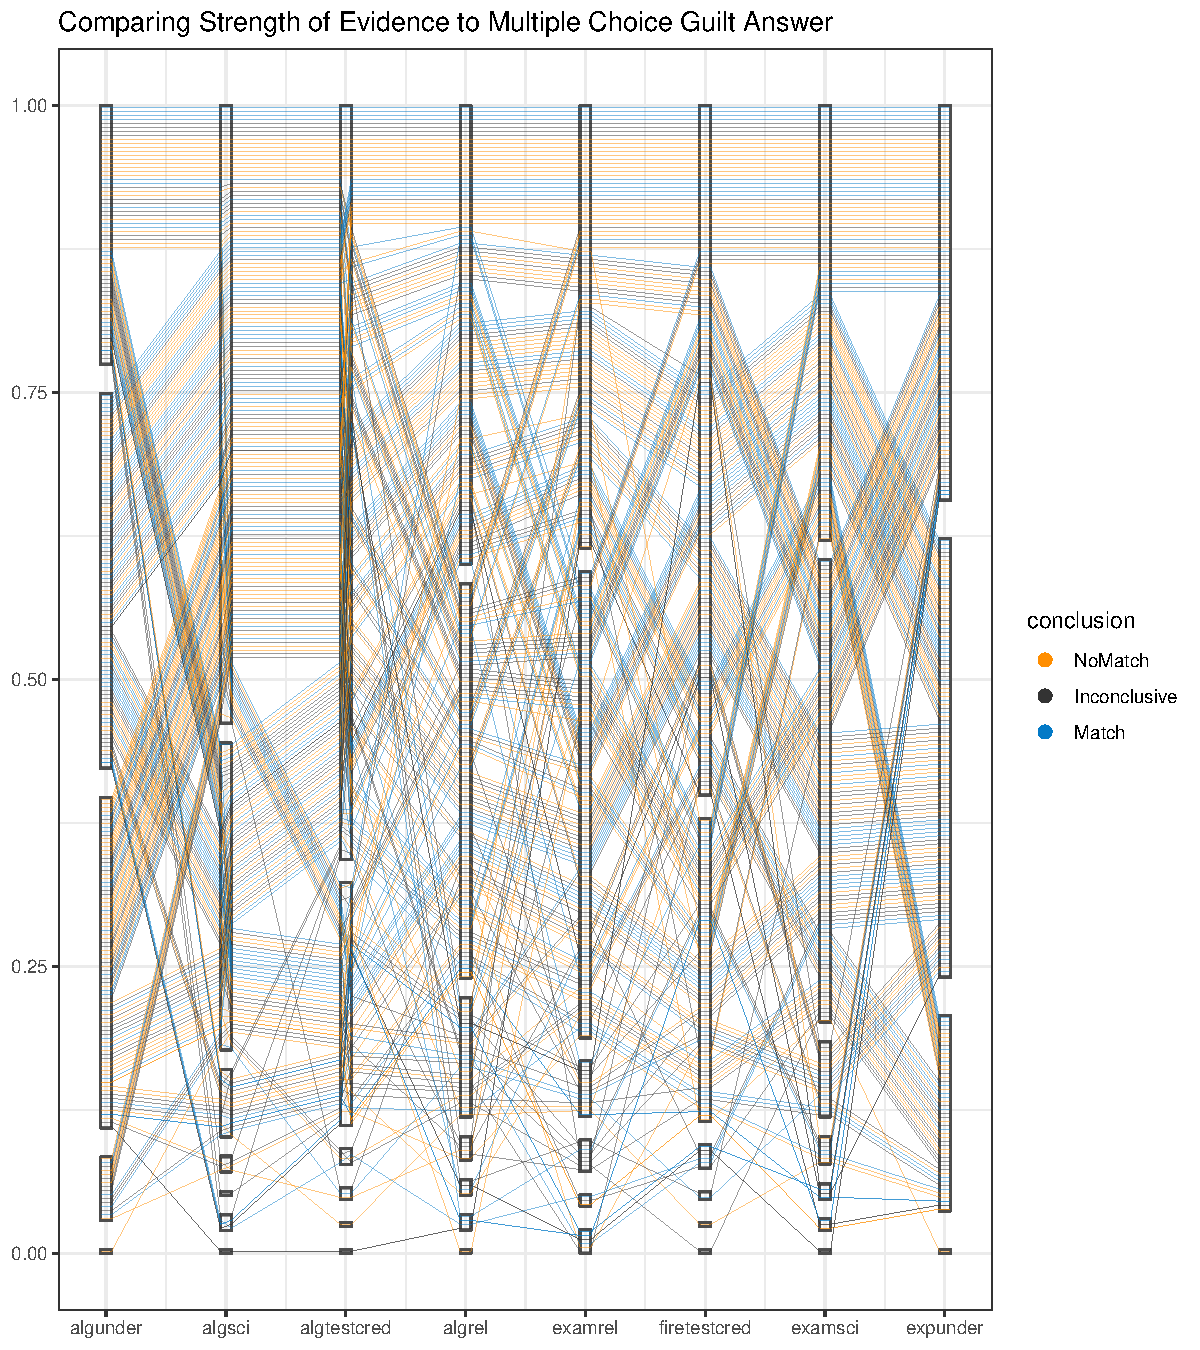
\includegraphics[width=\linewidth]{thesis_files/figure-latex/allpcp-1} \caption{Parallel Coordinate Plot for reliability, credibility, scientificity, and understanding}\label{fig:allpcp}
\end{figure}

Figure \ref{fig:allpcp} shows individual responses across all of the considered questions.
There were some individuals who selected the highest category for responses across the board, while others selected the highest response for all except their understanding of the algorithm.
In fact, algorithmic understanding seems to have the least consistent responses, based on the differences in the lines between algorithmic understanding and algorithmic scientificity.
These coordinate plots indicate that individuals tended to choose the same categories for the algorithm and the examiner across variables, with most variation between categories resulting from individuals moving up or down a single category.
Relatively few individuals changed their response by more than one category, when comparing between the algorithm and the expert.
These results generally reflect the trends shown in the histograms in the previous section.

\hypertarget{comments}{%
\subsection{Comments}\label{comments}}

Select comments are shown in Appendix \ref{select-comments}.
Many participants were concerned about the lawfulness of the arrest, and the lack of evidence tying the defendant specifically to the crime scene.
Several also indicate that they have pre-conceived notions, either about algorithms or about firearms evidence.
In particular, two comments were:

\begin{quote}
``Random forest methods for machine learning and classification are not very robust. They identify pictures of cats as hamburgers, for example. Just use science.''
\end{quote}

\begin{quote}
``Firearm evidence seems a lot like hair evidence which was debunked but I don't know that to be fact. From what was stated in this testimony, it seems to be mostly reliable but I wouldn't say it is strongly scientific.''
\end{quote}

The comments indicate that participants can have distrust for methods based on their previous ideas, which may not be factual.

\hypertarget{discussion}{%
\section{Discussion}\label{discussion}}

\hypertarget{summary-of-results}{%
\subsection{Summary of Results}\label{summary-of-results}}

As can be seen in most graphics, scale compression was an issue with this study.
The vast majority of participants selected the two highest categories for questions rating how credible, reliable, and scientific the expert/method was\authorcol{, despite following the scale size and labeling recommendations of } Groves et al. (2009).
This corresponds with B. Garrett \& Mitchell (2013)`s study of fingerprint match language, where they did not find a significant difference in the participants' feelings of guilt based on various match language.
B. Garrett \& Mitchell (2013) hypothesized that this may relate to strong feelings reliability for fingerprint evidence, resulting in individuals viewing any match as automatically reliable (without the need for stronger language).
\authorcol{In future studies, we will be evaluating different methods of response, aside from Likert scales, to study other formats that may yield less compressed results.}
People generally seemed to have less faith in inconclusive decisions.
They understood the examiner's comparison better than the algorithm comparison, which was expected given the statistical complexity of the algorithm procedure.
In general, participants also found the algorithm to be more scientific than the examiner, when presented with both methods.
The presence of images did not have a discernible effect in terms of credibility, reliability, or scientificity.
Participants' views of the credibility of the experts and the frequency with which firearms examiners make mistakes did not depend on the algorithm, images, or conclusion.

\hypertarget{limitations}{%
\subsection{Limitations}\label{limitations}}

Some of the major limitations for this project relate to the format and distribution of the survey material: the pool of participants, the format of the testimony, the limited testimony, and the inability to deliberate.
These limitations are also mentioned by B. Garrett et al. (2020).

Participants were limited to those who participate in online survey-taking websites.
These participants may not be representative of the US population, due to differences in computer access or use, occupation, or other such factors.
These factors may have an effect on study responses.
\authorcol{Another issue in representation results from the process of jury selection.}
\authorcol{Because individuals are not randomly approved for serving on a jury, the jury itself is unlikely to be composed of a representative sample of American citizens.}
Abramson (2018) \authorcol{argue that selection for jury duty does not result in a representative sample due to some courts' reliance solely on voter registration records for contacting eligible jurors, as well as large non response and non deliverable issues that are more prevalent in African American and Hispanic communities when compared to non-Hispanic White communities.}

Testimony was presented in a written format, which is unlike the courtroom setting of spoken testimony, where the jurors can see the experts.
However, the use of written testimony allowed for the use of gender-neutral names for the experts (Terry and Adrian), which may be more difficult to achieve in a courtroom or video setting.
Potential jurors may also develop views regarding the reliability/credibility of the examiner that are dependent on external factors - such as appearance or speech - rather than based on the testimony itself.

Testimony in this case was limited to only include the firearms evidence.
This led to some confusion on the part of the ``inconclusive'' and ``not a match'' scenarios, where there did not appear to be relevant evidence for the prosecution.
While the goal of this format was to ensure that participants focused on the bullet matching testimony (without the compounding influence of other witnesses or evidence), this would not be representative of courtroom testimony.

In a courtroom setting, jurors are able to deliberate with each other before reaching a conclusion with regards to the case.
These deliberations tend to be evidence-driven, as opposed to majority rule (Bornstein \& Greene, 2011, p. 65).
While the majority decision may be reflected in the final result, some studies suggest that juries tend toward leniency when there is not a definitive majority in a criminal trial (MacCoun \& Kerr, 1988).
The act of deliberation may result in different evaluations for Likert scale questions of reliability/credibility or strength of evidence than individual thought, even if a difference in guilty verdict rates are not found after deliberation for this simple case style.

There were several typos that were not corrected for approximately the first half of the participants.
For all scenarios, the firearms examiner was referred to as Alex Smith in the questions, whereas the name was Terry Smith throughout the testimony.
\authorcol{Several participants noted this discrepancy in their feedback on the survey, allowing us to fix the typo before all surveys were completed.}
\authorcol{There did not appear to be confusion due to the typo on the part of the participants.}
``Convenience'' was also misspelled in one question.
For exclusion testimonies, the name ``Alex Smith'' also occurred in the cross examination.
In the case of non-algorithm inconclusive testimonies, the question: ``Can you describe the process of obtaining these test fired bullets?'' was missing, but the response: ``The test-fired bullets came from a test fire of the gun recovered from the traffic stop.'' remained unchanged.
Due to the nature of the online survey, any differences caused by these typos would be confounded with demographics as well as date or time.

\hypertarget{future-research}{%
\subsection{Future Research}\label{future-research}}

One of the most notable features of the histograms presented in this research is the overwhelming proportion of respondents that selected the two highest categories, whether it be in terms of reliability, credibility, or scientificity.
The concentration of responses in the two highest categories may obscure potential differences in treatments, simply due to the issue of overall trust in the system.
It may also effect how well ordered logistic regression models fit the data.
This effect may be diminished through the use of jury instruction, and not referring to the firearms examiner or the algorithm witness as experts (as suggested by United States Courts for the Ninth Circuit (2019)).

Efforts are also being made to streamline the testimony into a single document, to prevent confounding typos.
Because the written court testimony may be difficult to follow and may give witnesses an air of impartiality, future studies will include images for relevant actors, and color coded speech bubbles to clarify which side the witness is speaking for.
We plan to develop a tool that can be used in testing courtroom scenarios, with versatile images for a variety of situations. These proposed changes can be seen in Appendix \ref{study-2-changes}.

An additional response to the study that was recorded is participants' note sheets.
Many participants copied and pasted portions of the testimony into their note sheets for later reference.
We plan to evaluate these note sheets, and develop a method for presenting the written notes alongside the testimony in order to produce a `heat map' of the text that participants found relevant.

\hypertarget{textcolor}{%
\chapter{Text analysis with Transcripts}\label{textcolor}}

\hypertarget{introduction-1}{%
\section{Introduction}\label{introduction-1}}

Note taking is commonly used when individuals are provided with a large amount of information that they may want to reference later.
These notes can act as a guide in terms of what items of information the note taker found most important.
By fluidly connecting notes from multiple note takers to the information presented, one may be able to discover the most `noteworthy' pieces of information, and compare the perception of the note takers to the goal of the presenter.
To this end, we have designed a method for highlighting presented information, in the form of a transcript, to correspond to the notes of participants in order to form a `heatmap' for the information that participants found worth recording. This method can provide valuable information about what participants chose to, or not to, record.
There were two important steps to this process: the text cleaning of cumulative notes, and the mapping of phrase frequency to form a `heatmap'.
The sequential note cleaning is necessary when participants take notes on a single notepad, but their notes are saved multiple times throughout the study as they were presented with new information.
By isolating the notes taken at each time point through text cleaning, we can isolate notes corresponding to the presentation of specific information.
This was accomplished through a combination of two methods (First N Character and Longest Common Substring) used to identify which notes have been added, presumably corresponding to the new information.
These individualized notes can then be mapped to the information presented through the use of collocations, or phrases of a set length.
Once the frequency with which each phrase of information appears in participant notes is calculated, this frequency can be mapped to a corresponding color to create a highlighting gradient that illuminates areas of participant focus.
This method was developed and tested on a trial transcript study designed to assess juror perceptions of the use of algorithms and demonstrative evidence in the courtroom.

\hypertarget{literature-review}{%
\subsection{Literature Review}\label{literature-review}}

\hypertarget{first-n-character-method}{%
\subsubsection{First N Character Method}\label{first-n-character-method}}

The First n Character (FNC) method relies on the concept of edit distance for matching and removing previous notes from sequential study documents.
I developed this method specifically for the cleaning of sequential notes.
In this process, a previous page's notes are matched to the next page's notes in order to remove duplicate text.
This is a form of pattern matching.
In a reference to algorithmic detection of plagiarism in computer programs, Parker \& Hamblen (1989) describe an algorithm that uses the character differences in order to compare how similar programs are.
Other algorithms \svp{discussed in} Parker \& Hamblen (1989) use code-specific features such as number of operators, lines of comments, and number of various loop statements.
Because we are only concerned with the content of the notes, there is little information to be gained from formatting; \svp{a notable difference from the plagiarism detection problem}.

There are \svp{many} examples of pattern matching in text analysis - such as Baeza-Yates \& Gonnet (1992) and Landau \& Vishkin (1988).
These papers rely on a set pattern to be found in the reference text, with a defined number of differences allowed between the pattern and the text.
According to Baeza-Yates \& Gonnet (1992), many algorithmic methods have been developed to solve this problem, with allowances for mismatches between the reference text and the pattern.
A similar allowance for differences is present in Landau \& Vishkin (1988), where differences are defined as either insertions, deletions, or substitutions.
This definition of differences is the same definition that is used in computing Levenshtein distance, also known as edit distance (Levenshtein, 1966).
Levenshtein considered the issue of insertions, deletions, and substitutions with binary code.
This concept has later been extended to include more extensive strings, as demonstrated by Konstantinidis (2005).
The edit distance can be used to determine the extent of matching text when comparing two sequential note sheets, in order to identify if a portion of notes should be removed.

\begin{longtable}[]{@{}
  >{\centering\arraybackslash}p{(\columnwidth - 8\tabcolsep) * \real{0.1406}}
  >{\centering\arraybackslash}p{(\columnwidth - 8\tabcolsep) * \real{0.1562}}
  >{\centering\arraybackslash}p{(\columnwidth - 8\tabcolsep) * \real{0.2812}}
  >{\centering\arraybackslash}p{(\columnwidth - 8\tabcolsep) * \real{0.1562}}
  >{\centering\arraybackslash}p{(\columnwidth - 8\tabcolsep) * \real{0.2656}}@{}}
\caption{Transformations used to calculate Edit Distance \label{tab:edist}}\tabularnewline
\toprule\noalign{}
\begin{minipage}[b]{\linewidth}\centering
Word 1
\end{minipage} & \begin{minipage}[b]{\linewidth}\centering
Word 2
\end{minipage} & \begin{minipage}[b]{\linewidth}\centering
Transformation
\end{minipage} & \begin{minipage}[b]{\linewidth}\centering
Method
\end{minipage} & \begin{minipage}[b]{\linewidth}\centering
Edit Distance
\end{minipage} \\
\midrule\noalign{}
\endfirsthead
\toprule\noalign{}
\begin{minipage}[b]{\linewidth}\centering
Word 1
\end{minipage} & \begin{minipage}[b]{\linewidth}\centering
Word 2
\end{minipage} & \begin{minipage}[b]{\linewidth}\centering
Transformation
\end{minipage} & \begin{minipage}[b]{\linewidth}\centering
Method
\end{minipage} & \begin{minipage}[b]{\linewidth}\centering
Edit Distance
\end{minipage} \\
\midrule\noalign{}
\endhead
\bottomrule\noalign{}
\endlastfoot
caw & cow & a → o & substitution & 1 \\
inveigh & neigh & \textcolor{gray}{i}n\textcolor{gray}{v}eigh & deletion & 2 \\
meow & homeowner & \textcolor{red}{ho}meow\textcolor{red}{ner} & insertion & 5 \\
Shire & Shareholder & i → a + \textcolor{red}{holder} & substitution and insertion & 7 \\
\end{longtable}

The edit distance is the number of characters that would need to be changed in order to transform the first string into the second string.
This includes insertions, deletions, and substitutions, in the case of the ``adist'' function (R Core Team, 2023).
These different transformations are shown in Table \ref{tab:edist}.
For example, ``caw'' and ``cow'' would have an edit distance of 1, because the strings match if the ``a'' is turned into an ``o''.
This is an example of substitution.
Similarly, ``inveigh'' and ``neigh'' would have an edit distance of 2, since 2 characters are deleted (``i'' and ``v'').
Finally, ``meow'' and ``homeowner'' would have an edit distance of 5, because 5 characters are added.
These operations can also be combined in edit distance calculations.
For example, going from ``Shire'' to ``Shareholder'' would require both a substitution and insertion.

Although edit distance can be used to calculate the similarity between notes, there is no set pattern that guarantees removal.
While the analysis is based on the previous page of notes, individuals do not always keep the previous page of notes the same - some delete parts, and some add new information in the middle.
Instead of only aiming to remove exact matches of the previous note sheet, we must factor in partial and discontinuous notes as well.

\hypertarget{longest-common-substring-method}{%
\subsubsection{Longest Common Substring Method}\label{longest-common-substring-method}}

Whereas calculating edit distance between two pages of notes is useful when finding notes that wholly match the previous page, the Longest Common Substring (LCS) method can be used to find pieces of notes that match between pages, so that this repeated text can be removed.
The LCS method accomplishes this goal through searching for common text between two sequential pages to be removed.
For example, in Figure \ref{fig:lcs}, the LCS between the two strings is ``the cat enjoys napping''.
In the process of note cleaning, this would be the string that is removed from the second page of notes, resulting in ``When it is quiet'' as the cleaned (non-repeated) notes.

\begin{figure}

{\centering 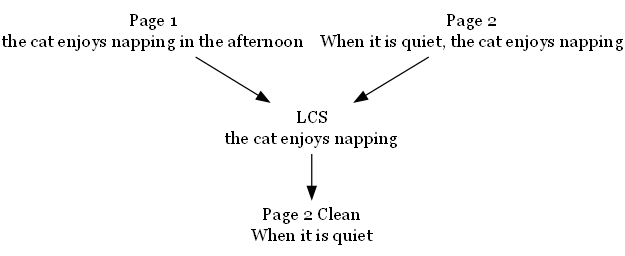
\includegraphics[width=\linewidth]{images/svg_graph} 

}

\caption{Longest Common Substring Diagram}\label{fig:lcs}
\end{figure}

Methods for computing the longest common substring between two sequences have been used to compare biological sequences (Crochemore, Iliopoulos, Langiu, \& Mignosi, 2017).
Solutions for finding the longest common substring \svp{utilize either} the construction of a suffix tree (Charalampopoulos, Kociumaka, Pissis, \& Radoszewski, 2021) or table (Landau \& Vishkin, 1988).
The suffix tree method is described by Gusfield (1997); in short, each unique suffix of a string would contribute a new branch to the suffix tree, where leaves consist of the string's terminal character: \$.

A solution implemented by Bielow, Mastrobuoni, \& Kempa (2016) in a CRAN R package constructs a matrix that records the length of a matching string at character \(i\) for string 1 (in the \(i\)th row), and character \(j\) for string 2 (in the \(j\)th column).
Because \svp{an} R implementation \svp{is readily available}, \svp{this is the solution used} for this analysis,
\svp{even though} Bielow et al. (2016) warns that this LCS method is inefficient, and meant to be used in small instances.
This method creates an empty matrix, where the number of rows correspond to the length of the first string, and the number of columns correspond to the length of the second string.
Thus, the first cell would correspond to the first character of both strings, and so on.
If the characters match and it is the first row or column, then the cell gets a value of 1.
If the characters match and it is not the first row or column, the the cell receives the value of the (i-1,j-1) cell plus one.
The first string's index for the substring of the longest length is saved.
This process is shown in Table \ref{tab:dylcs}, with two strings: ``gratuitous'' and ``intuitive''.
The diagonal of numbers in red indicate the longest substring, beginning and ending with `t'.
Thus, ``tuit'' is identified as the LCS.

\begin{longtable}[]{@{}lllllllllll@{}}
\caption{Dynamic Programming for LCS \label{tab:dylcs}}\tabularnewline
\toprule\noalign{}
\_ & g & r & a & t & u & i & t & o & u & s \\
\midrule\noalign{}
\endfirsthead
\toprule\noalign{}
\_ & g & r & a & t & u & i & t & o & u & s \\
\midrule\noalign{}
\endhead
\bottomrule\noalign{}
\endlastfoot
i & 0 & 0 & 0 & 0 & 0 & 1 & 0 & 0 & 0 & 0 \\
n & 0 & 0 & 0 & 0 & 0 & 0 & 0 & 0 & 0 & 0 \\
t & 0 & 1 & 0 & \textcolor{red}{1} & 0 & 0 & 1 & 0 & 0 & 0 \\
u & 0 & 0 & 0 & 0 & \textcolor{red}{2} & 0 & 0 & 0 & 1 & 0 \\
i & 0 & 0 & 0 & 0 & 0 & \textcolor{red}{3} & 0 & 0 & 0 & 0 \\
t & 0 & 0 & 0 & 1 & 0 & 0 & \textcolor{red}{4} & 0 & 0 & 0 \\
i & 0 & 0 & 0 & 0 & 0 & 1 & 0 & 0 & 0 & 0 \\
v & 0 & 0 & 0 & 0 & 0 & 0 & 0 & 0 & 0 & 0 \\
e & 0 & 0 & 0 & 0 & 0 & 0 & 0 & 0 & 0 & 0 \\
\end{longtable}

\hypertarget{collocation-analysis-and-fuzzy-matching}{%
\subsubsection{Collocation Analysis and Fuzzy Matching}\label{collocation-analysis-and-fuzzy-matching}}

After the notes are cleaned, sequences of 5 words (collocations) are used to find areas of the testimony that participants focus on.
For indirect matches, such as typos, weights are applied to these fuzzy matches to contribute to the total count.
While collocations traditionally refer to words that occur more frequently together - such as ``white house''(Merriam-Webster (2023)), tools for collocation analysis helpfully provide the frequency of occurrence for strings of a specified length (Schweinberger (2022)).

Character differences can effectively be used to indicate similarity between participants' notes and the text transcript.
This is useful in situation where individuals do not copy the notes directly.
In these cases, fuzzy matching can be used to find the transcript collocation that is the most similar to the participants' written notes.
This approximate string matching allows for matching strings that do not correspond directly (Gusfield (1997)), which allows for matching up participants' inexact notes with the closest transcript collocation.

In order to perform fuzzy matching on the indirect collocations from participants' notes, I used `stringdist\_join' from the `fuzzyjoin' R package (Robinson, 2020).
This function conducts a join with the best matching observations from the second dataset.
For example, consider asking young children to spell their birth month.
This may result in a dataset like Table \ref{tab:months}.

\begin{longtable}[]{@{}ll@{}}
\caption{Dataset of misspelled months \label{tab:months}}\tabularnewline
\toprule\noalign{}
Name & Month \\
\midrule\noalign{}
\endfirsthead
\toprule\noalign{}
Name & Month \\
\midrule\noalign{}
\endhead
\bottomrule\noalign{}
\endlastfoot
Billy & Mach \\
Jimmy & Apil \\
Frances & Mae \\
Gary & Febary \\
Steve & Octobr \\
Bobby & Agust \\
Tammy & Febrey \\
Greg & Agast \\
Benny & Jur \\
\end{longtable}

We may then want to match the written months to their correctly spelled counterparts.
While `stringdist\_join' will give values for all matches between the two data sets, we can \svp{then identify} the month that is closest to the misspelled value.

\begin{longtable}[]{@{}
  >{\raggedright\arraybackslash}p{(\columnwidth - 6\tabcolsep) * \real{0.1528}}
  >{\raggedright\arraybackslash}p{(\columnwidth - 6\tabcolsep) * \real{0.2639}}
  >{\raggedright\arraybackslash}p{(\columnwidth - 6\tabcolsep) * \real{0.1389}}
  >{\raggedright\arraybackslash}p{(\columnwidth - 6\tabcolsep) * \real{0.2222}}@{}}
\caption{\label{tab:fuzzymonth} Fuzzy Match by Month}\tabularnewline
\toprule\noalign{}
\begin{minipage}[b]{\linewidth}\raggedright
Month
\end{minipage} & \begin{minipage}[b]{\linewidth}\raggedright
Misspelled Month
\end{minipage} & \begin{minipage}[b]{\linewidth}\raggedright
Name
\end{minipage} & \begin{minipage}[b]{\linewidth}\raggedright
Edit Distance
\end{minipage} \\
\midrule\noalign{}
\endfirsthead
\toprule\noalign{}
\begin{minipage}[b]{\linewidth}\raggedright
Month
\end{minipage} & \begin{minipage}[b]{\linewidth}\raggedright
Misspelled Month
\end{minipage} & \begin{minipage}[b]{\linewidth}\raggedright
Name
\end{minipage} & \begin{minipage}[b]{\linewidth}\raggedright
Edit Distance
\end{minipage} \\
\midrule\noalign{}
\endhead
\bottomrule\noalign{}
\endlastfoot
June & Jur & Benny & 2 \\
July & Jur & Benny & 2 \\
March & Mach & Billy & 1 \\
August & Agust & Bobby & 1 \\
May & Mae & Frances & 1 \\
February & Febary & Gary & 2 \\
August & Agast & Greg & 2 \\
April & Apil & Jimmy & 1 \\
October & Octobr & Steve & 1 \\
February & Febrey & Tammy & 3 \\
\end{longtable}

In Table \ref{tab:fuzzymonth}, ``Month'' is the correctly spelled month, ``Misspelled Month'' is the child's spelling, and ``Edit Distance'' is the edit distance between the two words.
In this case, Benny's spelling (``Jur'') is equally close to ``June'' and ``July'', resulting in two listings.
This same concept is applied to matching collocations between a transcript and notepad.
In this case, the transcript is considered the ``correct'' version, and the participants' collocations that do not directly match are considered the misspellings.
This method finds the closest transcript collocation to the written collocation.

\hypertarget{implementation}{%
\section{Implementation}\label{implementation}}

\hypertarget{data-cleaning}{%
\subsection{Data Cleaning}\label{data-cleaning}}

\hypertarget{first-n-character-fnc-method}{%
\subsubsection{First N Character (FNC) Method}\label{first-n-character-fnc-method}}

\begin{longtable}[]{@{}
  >{\raggedright\arraybackslash}p{(\columnwidth - 6\tabcolsep) * \real{0.2542}}
  >{\raggedright\arraybackslash}p{(\columnwidth - 6\tabcolsep) * \real{0.3390}}
  >{\raggedright\arraybackslash}p{(\columnwidth - 6\tabcolsep) * \real{0.1695}}
  >{\raggedright\arraybackslash}p{(\columnwidth - 6\tabcolsep) * \real{0.2373}}@{}}
\caption{FNC Demonstration with an edit distance threshold of 3 \label{tab:fncmethod}}\tabularnewline
\toprule\noalign{}
\begin{minipage}[b]{\linewidth}\raggedright
Page 1
\end{minipage} & \begin{minipage}[b]{\linewidth}\raggedright
Page 2
\end{minipage} & \begin{minipage}[b]{\linewidth}\raggedright
FNC Edit Distance
\end{minipage} & \begin{minipage}[b]{\linewidth}\raggedright
FNC Page 2 Results
\end{minipage} \\
\midrule\noalign{}
\endfirsthead
\toprule\noalign{}
\begin{minipage}[b]{\linewidth}\raggedright
Page 1
\end{minipage} & \begin{minipage}[b]{\linewidth}\raggedright
Page 2
\end{minipage} & \begin{minipage}[b]{\linewidth}\raggedright
FNC Edit Distance
\end{minipage} & \begin{minipage}[b]{\linewidth}\raggedright
FNC Page 2 Results
\end{minipage} \\
\midrule\noalign{}
\endhead
\bottomrule\noalign{}
\endlastfoot
The cat ran & \textcolor{red}{The cat ran} up the tree & 0 & up the tree \\
The dog howled & \textcolor{red}{The cat ran up} the tree & 9 & The cat ran up the tree \\
The cat run & \textcolor{red}{The cat ran} up the tree & 1 & up the tree \\
\end{longtable}

In scenarios such as those shown in Table \ref{tab:fncmethod}, a straightforward method for note cleaning would be to measure the length of the page 1 notes (n), and compare the previous notes to the first n characters in the page 2 notes (shown in red) via edit distance.
If the edit distance is small (indicating a correspondence to the previous page's notes), the first n characters can be removed.
In the first row, the page 1 notes perfectly align with the beginning of the page 2 notes, resulting in an edit distance of 0, and the duplicate text would be removed.
In the second row, the text between the two pages differs significantly (edit distance of 9), so the page 2 notes are left alone.
The threshold of allowable disagreement between two strings can be controlled through setting the maximum allowable edit distance.
This concept is demonstrated in the third row, the text was edited from ``ran'' to ``run'', resulting in an edit distance of 1.
However, because the two texts have the same meaning, regardless of the typo, we would still want to remove the duplicate text.
By allowing for some mismatch between the two pages, we can account for inexact matches in the text cleaning.

This method works well when participants take notes sequentially.
In some instances, however, participants will delete portions of their previous notes, add new notes either before or in the middle of their old notes, or duplicate their old notes.
When participants delete a portion of their notes or add new notes before/in the middle of their old notes, the edit distance between the old and new notes could be large.
The first n character method cannot appropriately clean these notes, as shown in Table \ref{tab:issues}.

\hypertarget{longest-common-substring-lcs-method}{%
\subsubsection{Longest Common Substring (LCS) Method}\label{longest-common-substring-lcs-method}}

\begin{longtable}[]{@{}
  >{\raggedright\arraybackslash}p{(\columnwidth - 8\tabcolsep) * \real{0.1778}}
  >{\raggedright\arraybackslash}p{(\columnwidth - 8\tabcolsep) * \real{0.1778}}
  >{\raggedright\arraybackslash}p{(\columnwidth - 8\tabcolsep) * \real{0.2444}}
  >{\raggedright\arraybackslash}p{(\columnwidth - 8\tabcolsep) * \real{0.2444}}
  >{\raggedright\arraybackslash}p{(\columnwidth - 8\tabcolsep) * \real{0.1556}}@{}}
\caption{LCS Comparison for FNC Issues \label{tab:issues}}\tabularnewline
\toprule\noalign{}
\begin{minipage}[b]{\linewidth}\raggedright
Issue
\end{minipage} & \begin{minipage}[b]{\linewidth}\raggedright
Page 1
\end{minipage} & \begin{minipage}[b]{\linewidth}\raggedright
Page 2
\end{minipage} & \begin{minipage}[b]{\linewidth}\raggedright
LCS
\end{minipage} & \begin{minipage}[b]{\linewidth}\raggedright
Edit Distance
\end{minipage} \\
\midrule\noalign{}
\endfirsthead
\toprule\noalign{}
\begin{minipage}[b]{\linewidth}\raggedright
Issue
\end{minipage} & \begin{minipage}[b]{\linewidth}\raggedright
Page 1
\end{minipage} & \begin{minipage}[b]{\linewidth}\raggedright
Page 2
\end{minipage} & \begin{minipage}[b]{\linewidth}\raggedright
LCS
\end{minipage} & \begin{minipage}[b]{\linewidth}\raggedright
Edit Distance
\end{minipage} \\
\midrule\noalign{}
\endhead
\bottomrule\noalign{}
\endlastfoot
Deletion & The cat ran up the tree & The cat ran & The cat ran & 12 \\
Insertion & The cat ran up the tree & \textcolor{red}{The cat ran, chased by a} dog, up the tree & (The cat ran)(up the tree) & 11 \\
Duplication & The cat ran up the tree & \textcolor{red}{The cat ran up the tree} The cat ran up the tree & (The cat ran up the tree)(The cat ran up the tree) & 0 \\
\end{longtable}

The Longest Common Substring method is able to handle the issues found in the First n Character method, which is demonstrated in Table \ref{tab:issues}.
If notes are deleted, the LCS method can identify the substring from the previous notes, despite the large edit distance that would prevent removal in the FNC method.
If new notes are inserted in the middle of previous notes, the FNC method would compare the Page 1's notes with the red text of the Page 2 notes shown in the second row, resulting in an edit distance that would prevent removal.
With the LCS method, the first substring ``The cat ran'' could be identified and removed, then in a second iteration, the second substring of ``up the tree'' can also be removed, leaving only the new text.
In the case of duplication, the FNC method would be able to identify the first iteration of text that matches Page 1 and remove it; but it would not be able to identify the second occurrence of the text.
As before, the LCS method would be able to identify both instances through two iterations, and remove all Page 1 text.
In the case of the LCS method, a threshold must be picked for the minimum matching substring length to be considered `previous notes' and removed.
If the threshold is too small, the LCS method can identify words like ``the'' as matching previous testimony to be removed.
If the threshold is too large, the LCS method may be unable to remove substrings when new text is inserted in the middle of the old text.

\hypertarget{note-analysis}{%
\subsection{Note Analysis}\label{note-analysis}}

\hypertarget{collocations}{%
\subsubsection{Collocations}\label{collocations}}

In order to analyze which areas of the text individuals focus on, we must first find a way to compare their notes to the written testimony.
One way to do this comparison is through collocation analysis, which uses the frequency of strings of sequentially-appearing words (n-grams) in order to identify words that tend to `stick together'.
For example, in the case of the phrase ``The cat ran up the tree'', there would be three collocations of length 4, as shown in Table \ref{tab:colex}.
By matching the collocations that appear in the testimony to a frequency of the collocation from the participants' notepads, we can get frequency values for all n-grams that occur in the testimony.
The functions for creating highlighted text can be found in the package \texttt{highlightr} (Rogers \& VanderPlas, 2024a).

\begin{longtable}[]{@{}lllllll@{}}
\caption{Collocations in ``The cat ran up the tree'' \label{tab:colex}}\tabularnewline
\toprule\noalign{}
Collocation & The & cat & ran & up & the & tree \\
\midrule\noalign{}
\endfirsthead
\toprule\noalign{}
Collocation & The & cat & ran & up & the & tree \\
\midrule\noalign{}
\endhead
\bottomrule\noalign{}
\endlastfoot
1 & The & cat & ran & up & & \\
2 & & cat & ran & up & the & \\
3 & & & ran & up & the & tree \\
\end{longtable}

In setting the size of the collocation, there are two important factors to keep in mind: the frequency with which a phrase appears in the transcript itself, and the number of words in a row that individuals may directly copy from the transcript.
If the number of words considered in a collocation is too short, a phrase may occur multiple times throughout the transcript, without a way to distinguish which specific sections participants were recording.
For example, if we used a collocation of length two when analyzing an article about cats, a common phrase may be ``cats are''.
Because this phrase occurs frequently in the article, it does not by itself tell us if there are particular portions of the article that individuals find important, even if we add weights to calculate the relative frequency.
On the other hand, if we use a collocation of length 10, it is unlikely that a large amount of individuals copied the exact 10-word phrase, which results in fewer observations.
In considering these two issues, we decided on a collocation size of 5.
This would be long enough to avoid many common phrases, but short enough that individuals may copy the phrase down directly.
The implementation of collocations used the `quanteda' package (Benoit et al., 2018), with guidance from a tutorial by Schweinberger (2022).

Collocations are identified in the reference text, and assigned ordered word numbers (the first collocation of length 5 will have words 1-5, the second will have words 2-6, and so on).
This data structure is similar to that shown in Table \ref{tab:colex}, where the collocation is length 4 instead of 5.
These are then bound with collocations from the participants' notes based on the sequence of 5 words, in order to assign a frequency to each collocation.
We then take the average per word out of the possible collocations that the word could have appeared in.
For example, the first word can only appear in a single collocation (in Table \ref{tab:colex}, ``The'' only apprears in the first collocation, while ``ran'' appears in all three), so its average will be equal to the frequency of the first collocation.
When multiple 5-grams appear in the same reference text, the note frequency is divided by the number of appearances in the reference text in order to account for multiple occurrences.

These frequency values are then assigned to a color on a color scale in order to create a highlighting gradient.
We first implemented a graph of the testimony in `ggplot2' (Wickham, 2016) to assign color values to the frequencies based on a continuous gradient.
Then we used HTML gradient boxes, where the left color is that of the previous word, while the right color is based on the frequency of the current word.
This results in a smooth transition between words.

\hypertarget{fuzzy-matching}{%
\subsubsection{Fuzzy Matching}\label{fuzzy-matching}}

At times, participants do not directly copy a collocation, but the correspondence is clear enough to match their notes to the transcript.
In these cases, we can use fuzzy matching to account for indirect collocations.
Because the intent of the participant is more clear with simple typos (such as a single letter change) than with larger differences (such as the changing of multiple words), the count for these fuzzily matched observations are weighted based on the edit distance.
I set a maximum edit distance of 99 to be considered a match.
Specifically, a weight of \(\frac{1}{d+0.25}\) is used, where \(d\) represents the edit distance (between 1 and 99).
An edit distance of 0 would receive a weight of 1, since fuzzy matching need not be applied.
Another factor in the calculation is the number of matches per `misspelled' collocation.
To return to the month example shown in Table \ref{tab:fuzzymonth}, when Benny spelled a month ``Jur'', the edit distance to both ``June'' and ``July'' is 2.
It is then unclear which month Benny was born in, but they most likely meant June or July, as opposed to the other months.
Similarly, some collocation notes had the same edit distance for multiple transcript collocations.
In these cases, the frequency of the `misspelled' collocation notes are split evenly between the closest transcript collocations.
This results in a total fuzzy frequency per transcript collocation of:

\[
\sum_{i=1}^n\frac{x_i}{(d_i+0.25)c_i}
\]
where \(x_i\) is the count for the participant's note collocation \(i\), \(d_i\) is the distance between the transcript collocation and the `misspelled' collocation \(i\), and \(c_i\) is the number of transcript collocation matches for note collocation \(i\).
This quantity is then added to the count of direct collocation matches calculated in the previous section.

\hypertarget{standardization}{%
\subsubsection{Standardization}\label{standardization}}

In many study designs, the study transcript may differ in specific places due to the experimental conditions.
For clarity, when the study transcript corresponds across all scenarios, the frequency for all scenarios can be considered together.
When the testimony diverges, each scenario can be considered separately.
In order to consistently evaluate the frequencies throughout the transcripts, the final frequency count was standardized by the number of scenarios included.
This would result in collocations with a final frequency weight of:

\[
(z+\sum_{i=1}^n\frac{x_i}{(d_i+0.25)c_i})\frac{1}{ks}
\]

In this case, \(z\) is the count of direct matches; \(\sum_{i=1}^n\frac{x_i}{(d_i+0.25)c_i}\) is the weighted fuzzy match count as defined above; \(k\) is the number of times the collocation re-occurs in the transcript page itself; and \(s\) is the number of scenarios included in the frequency count.

\hypertarget{case-study}{%
\section{Case Study}\label{case-study}}

We applied this method to notes taken from a recent study on jury perception (described in Chapter \ref{study1}).
Participants were asked to read over a testimony transcript when the defendant had been charged with attempted robbery and answer some questions related to the scenario.
Conditions varied based on the examiner conclusion, the presence of images, and the presence of a bullet matching algorithm.
When the algorithm was present, participants also read the testimony of an algorithm developer, resulting in more pages of notes.
Participants were supplied with a notepad in order to take notes throughout the testimony.
We are interested in comparing this notepad to the given testimony, in order to determine which portions of the testimony the participants found to be worth recording the most.
Portions of the testimony that bear the most similarity to the collective notes will be have a highlight color on the higher end of the gradient color scale than testimony that appears less frequently in the collective notes.
The method outlined above resulted in scenario testimonies that indicate where participants copied notes.

\hypertarget{the-data}{%
\subsection{The Data}\label{the-data}}

Our study consisted of 560 uniquely recorded participants.
Of these 560 participants, 430 recorded something on the notepad.
This has resulted in 7,185 pages of notes with at least something recorded, out of 10,329 total pages.
For individuals who clicked through the survey multiple times but submitted a single result, the notes correspond to the closest time less than their submission time for observation per page number.
Note pages that corresponded to the questions (and not the testimony) were removed; this was above page 10 in conditions without the algorithm and page 19 in conditions with the algorithm.

\hypertarget{data-cleaning-1}{%
\subsection{Data Cleaning}\label{data-cleaning-1}}

In this study, participants were provided with a notepad to record information while reading through mock trial testimony.
Because participants are provided with the same continuous notepad throughout the study, the database records a \svp{snapshot} of their notes when they advance to the next page\svp{, providing a cumulative set of notes over time}.
Table \ref{tab:noteexample} is an example of what sequential notes may look like, taken from the second and third pages of a study participant's notes.

\begin{longtable}[]{@{}
  >{\raggedright\arraybackslash}p{(\columnwidth - 2\tabcolsep) * \real{0.1711}}
  >{\raggedright\arraybackslash}p{(\columnwidth - 2\tabcolsep) * \real{0.8289}}@{}}
\caption{\label{tab:noteexample} Participant Note Example}\tabularnewline
\toprule\noalign{}
\begin{minipage}[b]{\linewidth}\raggedright
page\_count
\end{minipage} & \begin{minipage}[b]{\linewidth}\raggedright
notes
\end{minipage} \\
\midrule\noalign{}
\endfirsthead
\toprule\noalign{}
\begin{minipage}[b]{\linewidth}\raggedright
page\_count
\end{minipage} & \begin{minipage}[b]{\linewidth}\raggedright
notes
\end{minipage} \\
\midrule\noalign{}
\endhead
\bottomrule\noalign{}
\endlastfoot
2 & discharge firearm in business- felony, not guilty \\
3 & discharge firearm in business- felony, not guilty ski mask.
no money, no injuries. 9mm, arrested after confiscated and
testing. \\
\end{longtable}

In order to appropriately clean the notes, the duplicated text (``discharge firearm in business- felony, not guilty'') needs to be removed from the third page, to leave only notes that correspond to the third page's testimony.
A generalized version of the functions used in this data cleaning are included in the \texttt{seqstrclean} package (Rogers \& VanderPlas, 2024b).

\hypertarget{method-comparison-study}{%
\subsubsection{Method Comparison Study}\label{method-comparison-study}}

The FNC and LCS methods for sequential notepad cleaning were first tested on a subset of notes resulting from a jury perception survey.
In order to compare the FNC and LCS methods described above, I manually cleaned a subset of the survey response notes to have a ``correct'' baseline with which to calculate error rates.
This dataset consists of 561 pages of `notes' (including 66 blanks) with 35 unique participants.
30 participants were randomly selected from the larger dataset \svp{to test the method's effectiveness}, while 5 participants were selected based on demonstrated issues with \svp{the existing} data cleaning \svp{process}.
The 5 selected participants included an individual who deleted almost all of the beginning notes; two individuals who pasted new notes in the middle of old notes; an individual who duplicated notes; and an individual who included the algorithm expert's trial confirmation as well as the forensic scientist's - duplicate text that should be included as the new notes.

Table \ref{tab:noteexample} shows two sequential note pages used in the method comparison dataset.
In this case, the FNC method could easily be applied; the page 2 notes perfectly align with the first part of the page 3 notes, resulting in an edit distance of 0 when comparing the first n characters of the third page.
Thus, by removing this beginning section, we would be left with the notes that are unique to page 3 - namely, ``ski mask. no money, no injuries. 9mm, arrested after confiscated and testing.''

For this method comparison study, I changed the FNC edit distance threshold with values of 0 character difference, 5 character difference, and 15 character difference (set as less than 1, less than 6, and less than 16).
In the method comparison study, I tried several different character length thresholds for the LCS method: 40 characters, half the previous note length, a third of the previous note length, and a fourth of the previous note length plus 5 (to compensate for shorter strings).

While the LCS method is able to solve the issues related to the First N Character method, such as cleaning notes that are not written sequentially, it has some issues of its own.
If the testimony itself contains duplicate text, such as the text related to swearing in witnesses, the LCS method would remove the new text that corresponds to the later testimony.
The other issue with the LCS method is the greater computational complexity.

\hypertarget{hybrid-method}{%
\paragraph{Hybrid Method}\label{hybrid-method}}

Due to the benefits and drawbacks of both the LCS and FNC methods, I investigated the use of a hybrid method in the hope that the FNC method could be used as a quick way to clean the simplest cases of notes, while the LCS method could be used to clean up the notes that are less clear-cut.
In order to determine which observations would need the second cleaning method, I created Figure \ref{fig:errorplot}.

\begin{figure}

{\centering 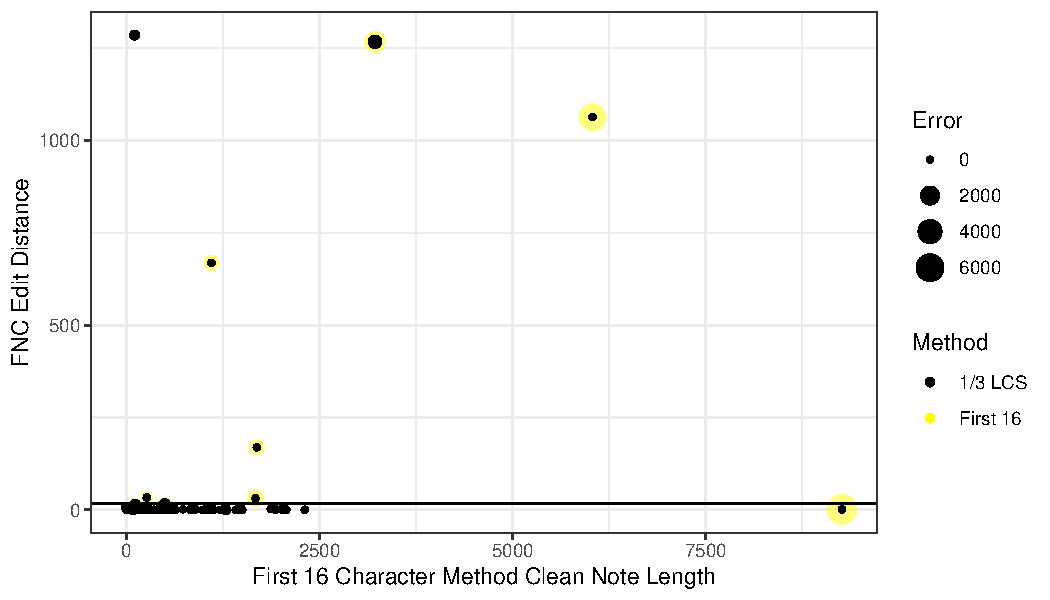
\includegraphics[width=\linewidth]{thesis_files/figure-latex/errorplot-1} 

}

\caption{Error Comparison}\label{fig:errorplot}
\end{figure}

Here, the yellow circles indicate the FNC method with a 16 character threshold, while the black circles represent the LCS method with a threshold of 1/3 the previous character length.
Larger circles indicate a larger amount of error when compared to the hand-cleaned notes.
The y-axis shows the edit distance computed between the current and previous notes for the FNC method, while the x-axis indicates the length of the clean notes.
The horizontal line is the 16 character threshold for the FNC method.
As can be seen, most observations are located in the bottom left of the graph, below the FNC threshold, and have relatively small circles.
These are notes where the FNC method was effectively applied, meaning that the edit distance was small enough to remove duplicated text at the beginning of the document.
In the observations above the threshold, most have a larger error when the FNC method is applied compared to the LCS method, with the exception of one observation in the top left.
In that case, the error appeared to be equal for both methods.
There is also a larger FNC method error for the observation on the bottom right of the graph.
This was a case of duplicate text, resulting in abnormally long notes.
This graph shows that an edit distance above the FNC method's threshold and the length of the cleaned notes can be used as criterion for determining when the LCS method should be applied.
I chose to set a threshold of 4 standard deviations above the mean note length for cleaned notes of the page of interest to constitute ``unusually long'' notes to apply the LCS method to.
I chose 1/3 of the previous notes as the LCS threshold because the mean edit distance to the correct notes was comparable to the 1/4 + 5 character threshold, but it is more conservative for larger notes (as can be seen in Table \ref{tab:cleancompare}).

\begin{table}

\caption{\label{tab:cleancompare}Note Cleaning Method Comparison}
\centering
\begin{tabular}[t]{l|c|c|c}
\hline
Method & Time (Minutes) & Error & SD\\
\hline
FNC 1 Character & 7.17 & 498.96 & 2769.83\\
\hline
FNC 6 Character & 3.74 & 201.35 & 1890.01\\
\hline
FNC 16 Character & 3.43 & 36.91 & 411.25\\
\hline
LCS 40 Character & 79.51 & 6.34 & 35.50\\
\hline
LCS 1/2 Previous Notes & 71.25 & 7.29 & 104.69\\
\hline
LCS 1/3 Previous Notes & 71.33 & 3.06 & 26.77\\
\hline
LCS 1/4 Previous Notes + 5 & 71.05 & 2.82 & 26.14\\
\hline
Hybrid (FNC 16 and LCS 1/3) & 4.52 & 2.13 & 24.62\\
\hline
\end{tabular}
\end{table}

The results of this study are shown in Table \ref{tab:cleancompare}.
Notably, the mean edit distance to the correct notes (or the error) is large for the FNC methods, with a high level of variation.
However, the computation time is between 3 and 8 minutes.
In the case of the LCS method, the error is much lower, but the computation time is above an hour, taking approximately 17 times as long as the FNC method.
The hybrid method combines the benefits of both of these methods.
The error rate is on par with that of the LCS methods, while the time is only slightly above that of the FNC methods.
The flowchart in Figure \ref{fig:flowchart} shows how this hybrid method will be applied to the case study dataset.

\begin{figure}

{\centering 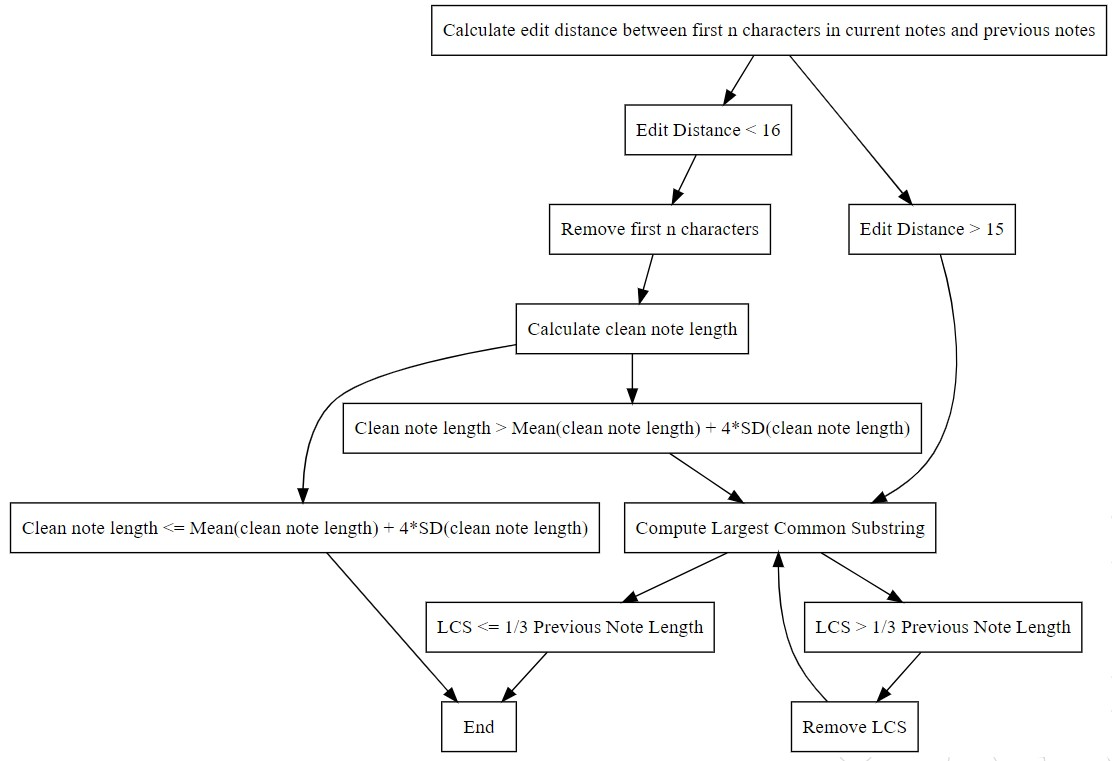
\includegraphics[width=\linewidth]{images/flowchart} 

}

\caption{Hybrid Flowchart}\label{fig:flowchart}
\end{figure}

\hypertarget{full-dataset}{%
\subsubsection{Full Dataset}\label{full-dataset}}

On the complete dataset, the hybrid method took a total of 19.33 minutes to run.
This demonstrates the time benefit of the hybrid method over the Longest Common Substring method - it took less time to clean the complete dataset with the hybrid method than it took to evaluate the reduced dataset with the LCS method.
The data cleaning resulted in a total of 2,372 note pages with some text recorded.
This is much smaller than the uncleaned total of 7,185 note pages, demonstrating a significant reduction in the note size (as is expected when removing the previous page's notes).

\begin{figure}

{\centering 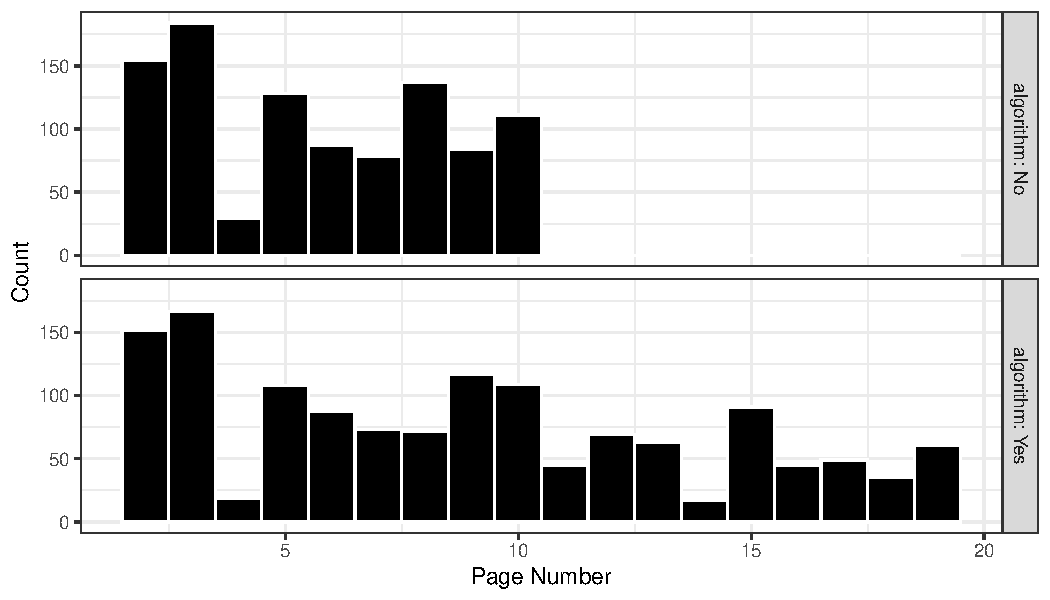
\includegraphics[width=\linewidth]{thesis_files/figure-latex/notecount-1} 

}

\caption{Number of Notes Taken Per Page}\label{fig:notecount}
\end{figure}

Figure \ref{fig:notecount} consists of the number of participants who took notes based on the page number.
In both the algorithm and the non-algorithm scenario, more individuals took notes on the first two pages of the testimony compared to the rest of the testimony.
However, the plot shows that individuals took notes throughout the testimony.

\hypertarget{collocation-analysis}{%
\subsection{Collocation Analysis}\label{collocation-analysis}}

Table \ref{tab:colcount} shows the highest frequencies for the second page of the testimony:

``In this case the defendant Richard Cole has been charged with willfully discharging a firearm in a place of business. This crime is a felony.
Mr.~Cole has pleaded not guilty to the charge.
You will now hear a summary of the case.
This summary was prepared by an objective court clerk.
It describes all of the evidence that was presented at trial.''

\begin{longtable}[]{@{}
  >{\raggedright\arraybackslash}p{(\columnwidth - 2\tabcolsep) * \real{0.1111}}
  >{\raggedright\arraybackslash}p{(\columnwidth - 2\tabcolsep) * \real{0.5694}}@{}}
\caption{\label{tab:colcount} Collocation Count for Page 2}\tabularnewline
\toprule\noalign{}
\begin{minipage}[b]{\linewidth}\raggedright
count
\end{minipage} & \begin{minipage}[b]{\linewidth}\raggedright
collocation
\end{minipage} \\
\midrule\noalign{}
\endfirsthead
\toprule\noalign{}
\begin{minipage}[b]{\linewidth}\raggedright
count
\end{minipage} & \begin{minipage}[b]{\linewidth}\raggedright
collocation
\end{minipage} \\
\midrule\noalign{}
\endhead
\bottomrule\noalign{}
\endlastfoot
134 & discharging a firearm in a \\
133 & firearm in a place of \\
130 & a firearm in a place \\
130 & in a place of business \\
\emph{121} & \emph{willfully discharging a firearm in} \\
\emph{93} & \emph{with willfully discharging a firearm} \\
\emph{91} & \emph{charged with willfully discharging a} \\
\emph{76} & \emph{been charged with willfully
discharging} \\
\emph{75} & \emph{cole has been charged with} \\
75 & has been charged with willfully \\
\end{longtable}

The italicized collocations in Table \ref{tab:colcount} show all of the collocations for the word ``willfully'' from the testimony above.
The frequencies for `willfully' can be averaged: \(\frac{121+93+91+76+75}{5}=91.2\).
This number will correspond to the shading of the word ``willfully'' in the highlighted testimony of Figure \ref{fig:highlights}.

Note that the words have a gradient.
This is to ensure a smooth transition between words in order to give an overall ``highlight'' effect, because we are interested in the important phrases in the testimony as opposed to the importance of individual words.

\begin{figure}

{\centering 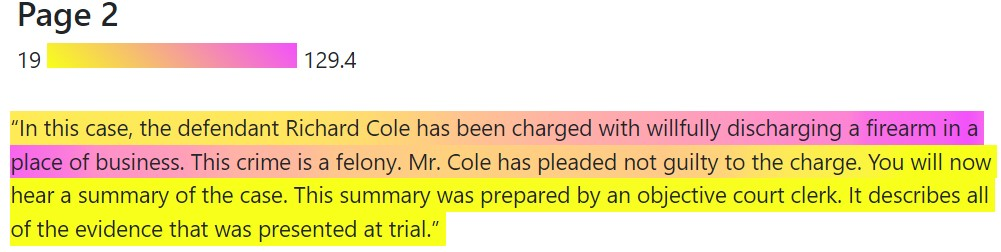
\includegraphics[width=\linewidth]{images/collocationanalysis} 

}

\caption{Collocation Count for Page 2}\label{fig:highlights}
\end{figure}

\hypertarget{fuzzy-matching-1}{%
\subsubsection{Fuzzy Matching}\label{fuzzy-matching-1}}

Table \ref{tab:fuzzyexam} demonstrates fuzzy matches on the testimony description text mentioned previously.
With an edit distance of 1, it can be seen that these fuzzy matches are the result of simple typos - making it clear which transcript collocation the misspelled version corresponds to.
While most collocation misspellings in the table only occur a single time (recorded via the ``Count'' column), the last collocation occurs twice - indicating that two individual note takers \svp{missed an} ``l'' \svp{in} ``willfully''.
The ``Collocation Matches'' column indicates if the participant's collocation matches with multiple collocations from the study - such as ``Jur'' in the example above.

\newpage
\begin{landscape}

\begin{table}

\caption{\label{tab:fuzzyexam}Close Fuzzy Matches from the Testimony}
\centering
\begin{tabular}[t]{l|l|r|r|r}
\hline
Transcript Collocation & Notepad Collocation & Edit Distance & Count & Collocation Matches\\
\hline
discharging
a
firearm
in a & discharing
a
firearm
in a & 1 & 1 & 1\\
\hline
the
defendant
richard
cole
has & he
defendant
richard
cole
has & 1 & 1 & 1\\
\hline
in a
place
of
business & in a
place
of
bussiness & 1 & 1 & 1\\
\hline
in
this
case
the
defendant & n
this
case
the
defendant & 1 & 1 & 1\\
\hline
willfully
discharging
a
firearm
in & wilfully
discharging
a
firearm
in & 1 & 2 & 1\\
\hline
\end{tabular}
\end{table}

\begin{table}

\caption{\label{tab:fuzzyexamlarge}Distant Fuzzy Matches from the Testimony}
\centering
\begin{tabular}[t]{l|l|r|r|r}
\hline
Transcript Collocation & Notepad Collocation & Edit Distance & Count & Collocation Matches\\
\hline
describes
all
of
the
evidence & information
presentation
and
demonstrative
evidence & 32 & 1 & 1\\
\hline
that
was
presented
at
trial & trial
information
presentation
and
demonstrative & 30 & 1 & 1\\
\hline
the
evidence
that
was
presented & perception
of
trial
information
presentation & 29 & 1 & 2\\
\hline
evidence
that
was
presented
at & perception
of
trial
information
presentation & 29 & 1 & 2\\
\hline
\end{tabular}
\end{table}

\end{landscape}

Interestingly, when considering the most distant fuzzy matches in Table \ref{tab:fuzzyexamlarge}, these phrases do not come from simple typos, but rather from a non-testimony title portion of the study: ``Jury Perception of Trial Information, Presentation, and Demonstrative Evidence'', and may result from participants copying the entire web page into the note sheet.
Two individuals copied this title into their notes, but on different pages of the testimony.
The collocations in Table \ref{tab:fuzzyexamlarge} correspond to the individual who copied the title on the second page of the testimony.
Because these phrases do not noticeably correspond to the transcript collocations, as shown in their larger edit distance, they are given less weight.
In this case, we also see that the participant collocation of ``perception of trial information presentation'' was an equal edit distance from two collocations, based on the ``Collocation Matches'' value.
Thus, the weight would be adjusted accordingly due to the presence of two close matches.

\hypertarget{standardization-1}{%
\subsubsection{Standardization}\label{standardization-1}}

The courtroom transcript testimony comes from a 2x2x3 factorial design (presence or absence of images, presence or absence of the algorithm, and the conclusion: identification, inconclusive, or elimination).
This standardization is included in Figure \ref{fig:weightedhighlights}.
In comparing with the unweighted highlighting without fuzzy matching of Figure \ref{fig:highlights}, the same pattern emerges in terms of phrase popularity: most individuals focused on the crime.
However, the numerical values of the gradient scale have changed.

\begin{figure}

{\centering 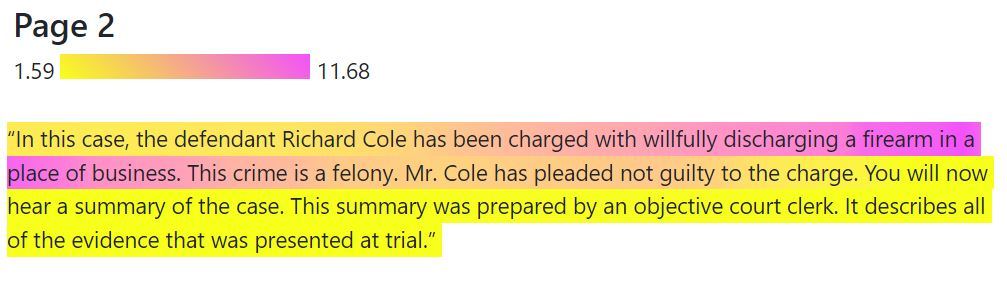
\includegraphics[width=\linewidth]{images/weightedcollocationanalysis} 

}

\caption{Highlighted Fuzzy Collocation for Page 2}\label{fig:weightedhighlights}
\end{figure}

\hypertarget{final-output}{%
\subsection{Final Output}\label{final-output}}

This final note analysis, which includes fuzzy matching, can be found at \url{https://rachelesrogers.github.io/Presentations/Collocations/Collocation\%20Comment\%20Analysis\%20Cleaned.html}.
In visually comparing the highlighted transcripts for fuzzy matches to those without fuzzy matching, the results appear to be fairly similar.
While the fuzzy matching did increase the frequency number, the overall trends remained the same for the dataset.
This can be seen in Table \ref{tab:nonfuzzycount}.
The ranking of the collocations remains is similar, aside from differences that can be seen in collocations that had the same non-fuzzy count.

\begin{table}

\caption{\label{tab:nonfuzzycount}Table of Collocation Frequencies}
\centering
\begin{tabular}[t]{l|c|c}
\hline
collocation & Nonfuzzy & Fuzzy\\
\hline
discharging a firearm in a & 134 & 151.21\\
\hline
firearm in a place of & 133 & 139.44\\
\hline
a firearm in a place & 130 & 137.02\\
\hline
in a place of business & 130 & 136.70\\
\hline
willfully discharging a firearm in & 121 & 136.48\\
\hline
with willfully discharging a firearm & 93 & 107.61\\
\hline
charged with willfully discharging a & 91 & 101.98\\
\hline
been charged with willfully discharging & 76 & 83.32\\
\hline
cole has been charged with & 75 & 76.32\\
\hline
has been charged with willfully & 75 & 78.77\\
\hline
\end{tabular}
\end{table}

The standardized frequency values remain fairly consistent throughout the testimony.
Some areas that individuals focused on were the crime and its extent (in terms of injury), the qualifications/process of the firearms examiner, and the results from the analysis.
While this type of analysis may allow us to determine the areas that participants copied into their notes, it does not indicate why the participants found this testimony worth copying.
This may either indicate areas that participants saw as interesting or confusing, or a mixture of both.

\hypertarget{discussion-1}{%
\section{Discussion}\label{discussion-1}}

\hypertarget{conclusion-1}{%
\subsection{Conclusion}\label{conclusion-1}}

Overall, this process effectively cleans and displays notes with the desired highlight format.
For sequential notes, such as this case, the First N Character method manages to clean the notes in most cases.
In the cases where the FNC method is ineffective (when the edit distance is above the threshold or the clean notes are unusually long), the Longest Common Substring method can be applied.
This process was demonstrated in a dataset of 35 participants, and showed a significant note reduction on the full dataset.

After the notes are cleaned, collocations can be used to determine what phrases participants decided to copy into their notes.
The length of the collocation was chosen to be long enough to avoid commonly repeated phrases, but short enough that participants may directly copy the phrase into their notes.
Notes that were not directly copied were included with weights proportional to edit distance through the use of fuzzy matching.
The final output qualitatively indicates which portions of testimony participants found relevant to copy.

This method opens up new avenues for user studies and analyses.
While this method was developed for a specific use case, it has diverse applications, including education, social science, and more.
These methods are being developed into R packages to be used by other
researchers in transcript analysis.
Future studies may investigate the application of this notepad in a variety of scenarios, such as course notes or collaborative note
taking.
Another application of this type of analysis may be used in the evaluation of student note taking or Wikipedia article edits.

\hypertarget{study2}{%
\chapter{An Investigation of Response Types}\label{study2}}

\hypertarget{background-1}{%
\section{Background}\label{background-1}}

\hypertarget{problems-in-study-1}{%
\subsection{Problems in Study 1}\label{problems-in-study-1}}

The results from the initial study found in Chapter \ref{study1} call into question the use of Likert response scales when evaluating jury perception of firearms experts, as well as the use of a transcript testimony format.
Responses pertaining to the credibility of the expert, as well as the reliability and scientificity of the evidence, suffered from scale compression when a Likert scale was used - participants indicated overall confidence in credibility, reliability, and scientificity by mainly selecting the two highest categories of each scale.
This lack of variation in scale responses makes it difficult to discern potential differences between treatment conditions.
Due to this difficulty, we conducted a follow-up study comparing various response types, in order to determine substitute questions that may result in a wider distribution of responses. \svp{I think you may want to have a few references about why scale compression is bad and how to deal with it as part of the intro here?}

\authorcol{According to }Groves et al. (2009)\authorcol{, an error in survey measurements may result from a difference between the construct that we wish to evaluate, and the measurement used to evaluate it.
In this case, there is a disconnect between what we want to measure (participant's perception of the witness/method's abilities) and what we ended up measuring with Likert scales (reliability, credibility, and scientificity).
This disconnect can be seen in the form of scale compression: due to the limited scale, we are unable to observe individuals' true perceptions with regards to the witnesses and methods.}
Groves et al. (2009) \authorcol{ uses the National Assessment of Educational Progress as an example of the difference between construct and measures: "when measuring the construct of mathematical abilities of 4th graders, the measures are sets of arithmetic problems" (50).
The scale compression seen in our initial study would be equivalent to using the wrong set of arithmetic problems: if the problems are simple enough that almost all 4th graders receive a perfect score, then the true mathematical abilities of the 4th graders are not being evaluated.
Similarly, the standard for being considered reliable, credible, and scientific as a court-approved witness or method is too easy to overcome.}

In investigating scale compression, we found that United States Courts for the Ninth Circuit (2019) suggests that the use of the term ``expert'' may result in jurors giving the testimony more weight, and \authorcol{suggests judges use the following jury instruction:}

\begin{quote}
\authorcol{"You [have heard] [are about to hear] testimony from [name] who [testified] [will testify] about [his] [her] opinions and the reasons for those opinions.  This opinion testimony is allowed because of the specialized knowledge, skill, experience, training, or education of this witness.
Such opinion testimony should be judged like any other testimony.  You may accept it or reject it, and give it as much weight as you think it deserves, considering the witness’s knowledge, skill, experience, training, or education, the reasons given for the opinion, and all the other evidence in the case."}
\end{quote}

Additional cross examination testimony with regards to the firearms examiner's inability to specifically tie the defendant to the crime scene is included as well, due to a lack of distinction in participants between evidence tying the firearm to the crime scene, and evidence tying the defendant to the crime scene.
As in the initial study, these changes were directly related to trial transcripts or resources.
The transcript changes for the second study can be found in Appendix \ref{study-2-changes}.

In the initial study, some participants were confused about \authorcol{the witness testimony:}

\begin{quote}
\authorcol{"Very difficult for juror to understand and remember the scientific evidence."}
\end{quote}

\authorcol{Other participants thought that the defendant was convicted, although this is not specified in the transcript:}

\begin{quote}
\authorcol{"Going by what I read and reviewing my notes I see that the firearms evidence was inconclusive against R. Cole.} \emph{So I am baffled as to why he was convicted.} \authorcol{[emphasis added] Also I prefer more things like visual evidence via a good quality video camera. Or a whole group of people testifying against someone saying things like they saw, they heard, or they know someone is prone to commit certain crimes."}
\end{quote}

\begin{quote}
\authorcol{"I would have like another firearms expert testify or a representative from that 9mm handgun manufacturer explain how and why each individual handgun are designed such that the lands and grooves create unique impressions on bullets for each gun. I do believe the firearms expert and his credibility.} \emph{Further, the defendant would be basically convicted only on one evidence.} \authorcol{[emphasis added] Would have liked to read or know what was his alibi during that attempted robbery and if a search warrant issued to search for that ski mask. What about security cameras to determine any other physical identification. This case presentation was scant and focused too heavily on one piece of evidence and testimony."}
\end{quote}

The testimony transcript format did not clearly identify the speaker with each line, instead using ``Q:'' and ``A:'' in most cases, as shown in Appendix \ref{study-2-changes}.
The lack of visual cues for \svp{matching text with the speaker} is not representative of the courtroom setting.
The transcript format may also lend an air of impartiality to the witnesses due to the relatively unclear identity of the individual asking the questions.
\authorcol{In order to clarify, we also added} testimony where the prosecution called the witness to testify, instead beginning with the swearing in of the witness.
Due to this issue, we strove to develop a general tool that can be used in online courtroom studies to provide visual representation of relevant actors, making it easier to track speakers, and with versatility in terms of individual characteristics.
\authorcol{These changes are shown in Figure} \ref{fig:testimonyformat}.

\begin{figure}

{\centering 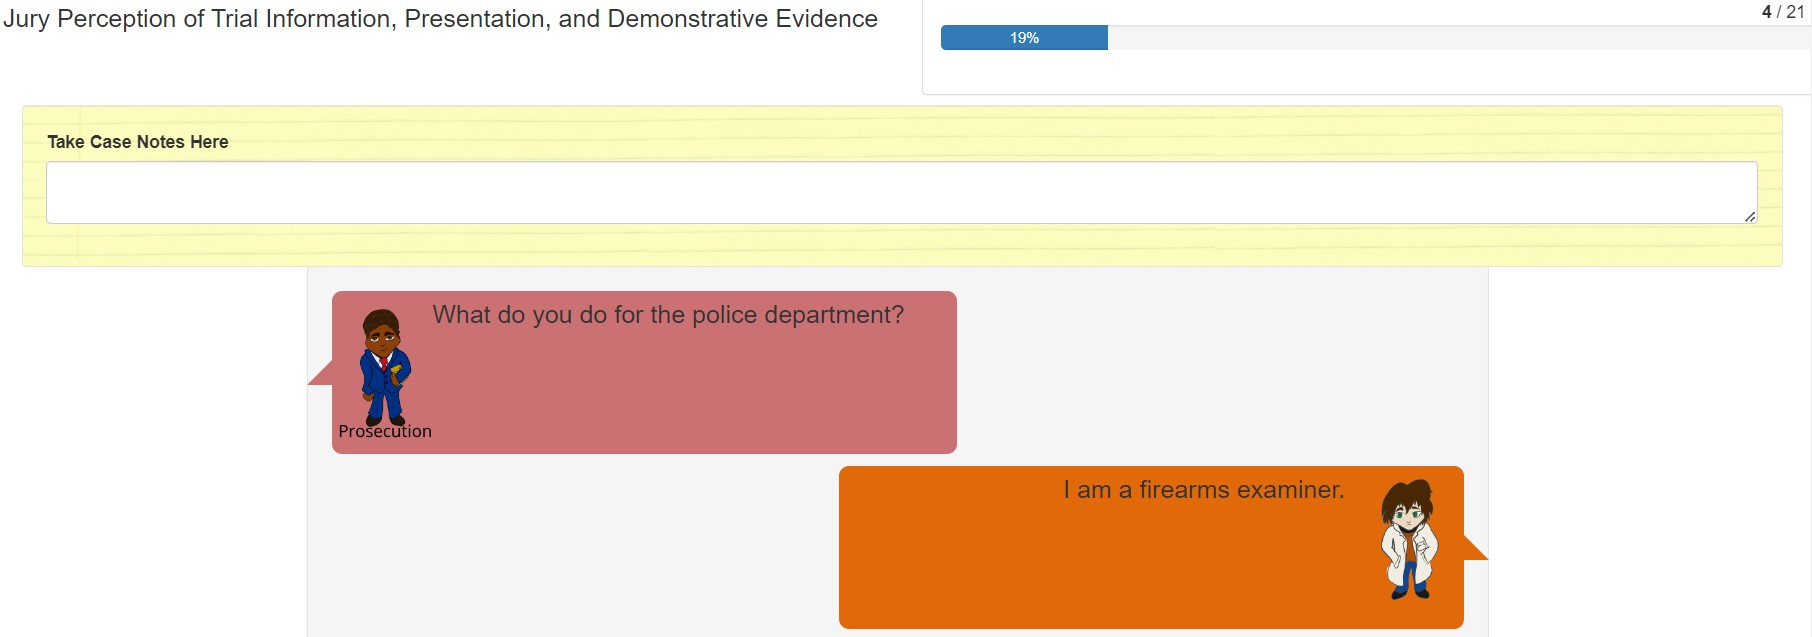
\includegraphics[width=\linewidth]{images/Study2_Screenshot} 

}

\caption{A screenshot of the layout of the second study.}\label{fig:testimonyformat}
\end{figure}

In order to minimize the chance of confounding typos as seen in Study 1, we used one master file with all lines of testimony, labelled by the scenario in which the testimony occurs, \svp{which minimizes the need to change testimony in multiple locations}.
\svp{In addition,} this format allows for more flexibility when implementing the R Shiny application.
We also use unique identification throughout the database files in the form of Prolific ID's and a random number assigned to the participant \svp{upon initial connection to the application} instead of relying on \svp{browser-based} fingerprints, which resulted in technical difficulties in a preliminary run of this second study, so the demographics section can more easily be linked to the final results.

\authorcol{Individuals also indicated confusion with regards to the use of a partial testimony transcript:}

\begin{quote}
\authorcol{"Thank you for conducting this study. Where's the defense in all of this? It would have been  helpful to know whether or not the defendant had an alibi, whether his firearm had in fact been recently fired, from a forensics perspective, whether there were any in-store or exterior or neighborhood cameras that picked up whoever discharged the firearm. Convenience stores nearly always have a height chart posted alongside the door but no one provided an approximate height or weight for the person who discharged the firearm. This was an interesting study. All the best to your research team in this and  your future endeavors. "}
\end{quote}

\begin{quote}
\authorcol{“It would be interesting to know if the prosecution would order a second
testing of the gun with a different expert. Also why would the prosecution
charge this man since it had no eyewitnesses or other evidence placing him at
the scene of the robbery at the time of the robbery and since the gun found in
the defendant was not a match to the bullet found at the scene. Charging him
seems pointless as there’s virtually no evidence other than he owned a 9mm
handgun.”}
\end{quote}

\authorcol{Due to this confusion, an additional line is added to the study description to clarify that this is not the only evidence presented in the case.}

\hypertarget{study-visualization}{%
\subsection{Study Visualization}\label{study-visualization}}

\begin{figure}

{\centering 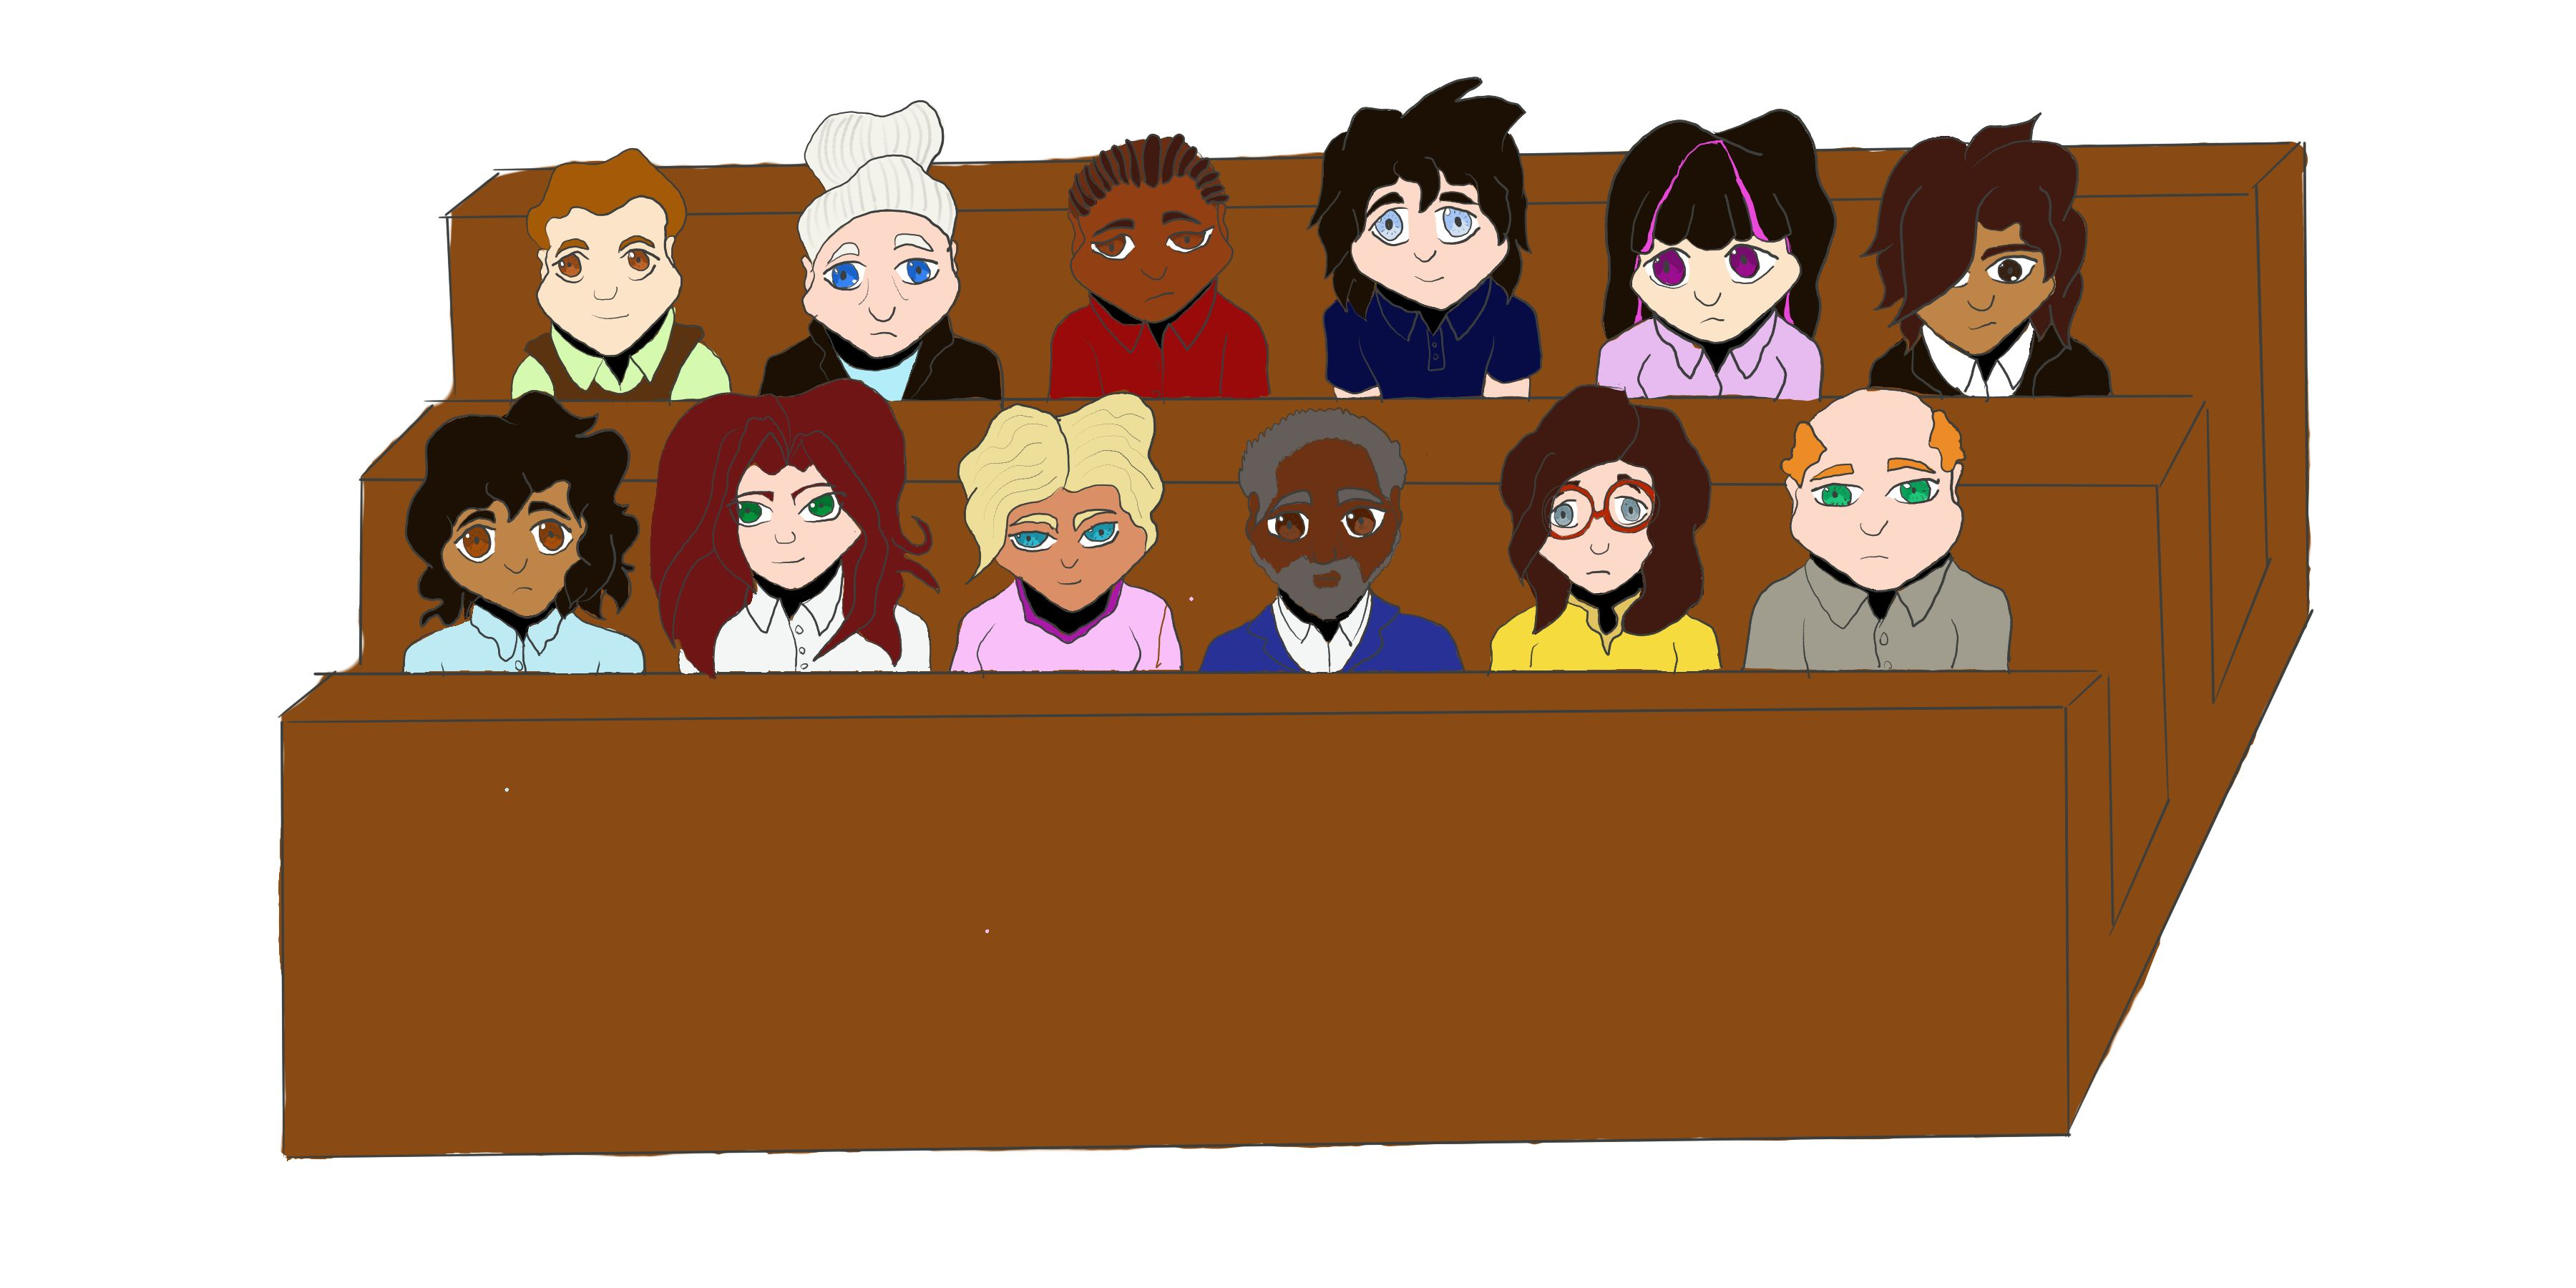
\includegraphics[width=\linewidth]{images/Jury} 

}

\caption{An image of the jury panel}\label{fig:jurypanel}
\end{figure}

Figure \ref{fig:jurypanel} and Figure \ref{fig:testimonyformat} show some of the characters that have been developed for this study (drawn by Richy Meleus), as well as a screenshot of the study format.
These characters were drawn so that the clothes and heads can be interchanged, providing a wide variety of characters for potential scenarios.
One difficulty in including drawn figures with realistic skin tones and figures is the influence of perceived race or gender on participant judgments.
Stanley, Sokol-Hessner, Banaji, \& Phelps (2011) found a relationship between implicit racial bias and the perceived trustworthiness of individuals based on images of black and white males.
They also found that 80\% of participants exhibited pro-white implicit bias.
Because of this potential bias introduced by visual figures, we plan to conduct a follow-up study in order to determine how these figures are perceived \svp{as part of the validation of this set of figures for wider use}.
For the current study, the same figures are used consistently across all conditions to prevent a confounding effect.

To investigate a which response type may be most informative for this study and to troubleshoot the use of figures and speech bubble format, we conducted a micro study using various response types.
\authorcol{As discussed in the Literature Review in Chapter} \ref{litreview}\authorcol{, there are many issues with recording participant responses in a manner that best represents the construct of interest.
While the question we followed in Chapter} \ref{study1} \authorcol{mainly aligns with the recommendations of these authors, in terms of the use of 7 and 9-point Likert scales with labelled categories, these scales failed to capture the underlying attitudes that we wished to address.
Based on these recommendations, adding more categories to the Likert scales would not be recommended, leading us to search for other methods of response.
However, participants may find the use of numerical scales to be difficult to use, so these scales must be investigated for consistency.}

\hypertarget{methods-1}{%
\section{Methods}\label{methods-1}}

\hypertarget{study-format-1}{%
\subsection{Study Format}\label{study-format-1}}

Participants were presented with the same scenario described in Chapter \ref{study1}: participants read a trial transcript regarding an attempted convenience store robbery, where the only evidence presented is a bullet comparison between the defendant's gun and a bullet recovered from the scene of the crime (a scenario from B. Garrett et al. (2020)).
In this case, however, the only factor that was changed was the conclusion of the firearms examiner: either an indentification or exclusion.
In all conditions, the algorithm was absent and there were no images \svp{provided as demonstrative evidence during testimony}.
The testimony largely followed that of Chapter \ref{study1}, aside from differences in the format and additional testimony described above and outlined in Appendix \ref{study-2-changes}.
In this case, it was also explicitly stated that the testimony did not reflect all evidence presented in the case, because in the exclusion condition there \svp{is clearly insufficient} evidence to bring the case to trial.
Figure \ref{fig:responsefigures} depicts the characters used in this study.
Those speaking on behalf of the prosecution were coded with speech bubbles in warmer colors (red for the prosecutor and orange for the forensic scientist), while the defense was coded with a cooler color (purple), and the judge was coded as grey.

\begin{figure}

{\centering 
\includegraphics[width=\linewidth]{thesis_files/figure-latex/responsefigures-1} 

}

\caption{Figures used in the response study. From left to right: the judge, forensic scientist, prosecutor, and defense lawyer.}\label{fig:responsefigures}
\end{figure}

At the end of the testimony, the participants were asked a variety of questions regarding the strength of evidence in the case.
\authorcol{All questions asked in this study are shown in Figure} \ref{fig:questions}.
Questions of probability, strength of evidence, and decision to convict were repeated from the Chapter \ref{study1} study.
Participants were asked to evaluate the probability that the defendant committed the crime, both with a visible probability scale (allowing the participants to select the exact probability integer) and with a non-visible scale (only the numbers of 0 and 100 were available on the extremes of the scale).
The strength of evidence was a Likert scale with values from ``Not at all strong'' to ``Extremely strong'' with nine points.
In terms of conviction, participants were reminded of the decision criterion of ``beyond a reasonable doubt'' when making a decision in a criminal trial, and asked if they would choose to convict.

\begin{figure}

{\centering 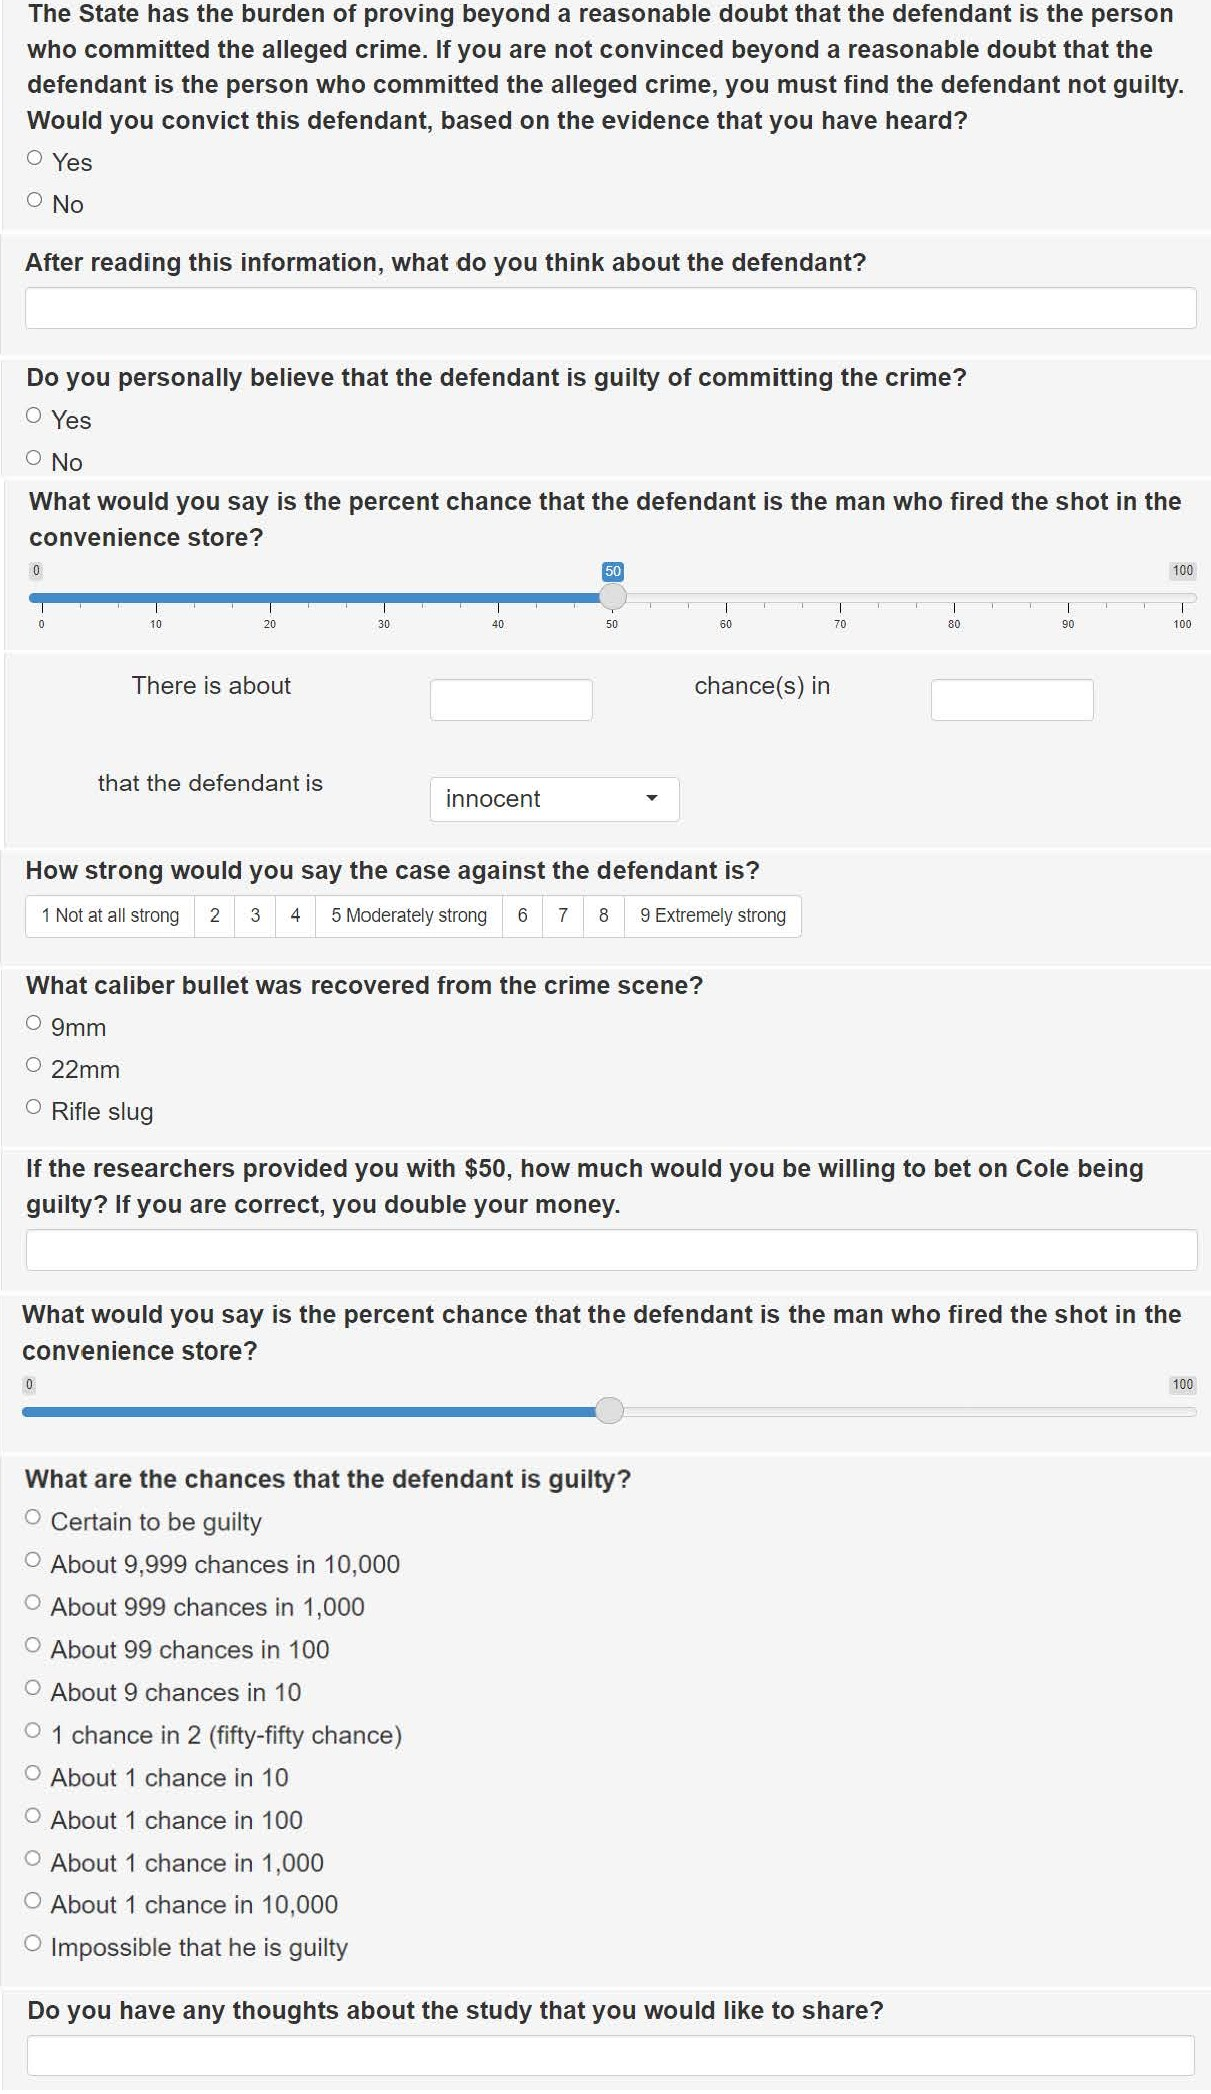
\includegraphics[width=\linewidth]{images/study_questions} 

}

\caption{Questions asked in the Response Survey}\label{fig:questions}
\end{figure}

New questions for this response study asked individuals to give their opinion of the guilt of the defendant, as well as assessing the chances that the defendant committed the crime, how much they would be willing to bet that the defendant was either innocent or guilty, and their opinion of the defendant.
In addition to a question regarding whether or not the participant would choose to convict, we also asked the participants to give their personal opinion on the guilt of the defendant.
This provides a second threshold for assessing the strength of evidence, aside from the ``beyond a reasonable doubt'' standard.

Two different questions were asked with regards to the chances that the defendant committed the crime.
One was in a multiple choice format, with extreme values of ``Impossible to be guilty'' and ``Certain to be guilty'', and intermediate values ranging from ``About 1 chance in 10,000'' to ``About 9,999 chances in 10,000'' with denominator values changing by a decimal place for each choice, and a middle value of ``1 chance in 2''.
This format was taken from Thompson \& Newman (2015)'s study of DNA, which consisted of larger scaled values in the denominator (up to 1 in 10 million).
The second question allowed participants to select both the numerator and denominator: ``About \_\_\_ chance(s) in \_\_\_ that the defendant is (innocent/guilty)'', where participants were able to select to express the value as innocence or guilt (the default value was ``innocent'').
In the preliminary study, participants had to express chances that corresponded with their opinion on the defendant committing the crime, but this resulted in some scale confusion.
In both cases, the numerator had to be less than or equal to the denominator, \svp{restricting the numerical result to the $[0,1]$ range.}

Individuals who thought that the defendant was guilty were asked how much they were willing to bet that the defendant was guilty, if hypothetically researchers provided them with \$50 and they would double their money if they were correct, and vice versa.
A final new question was open ended, and asked participants to provide their opinion of the defendant.
We first asked individuals to provide their opinion of the defendant, their conviction decision, and their personal opinion of the guilt of the defendant.
All other questions were randomized \svp{subject to the constraint that} the two probability questions and the two chance questions were not \svp{adjacent}.

\hypertarget{prolific-1}{%
\subsection{Prolific}\label{prolific-1}}

Participants were recruited in a similar manner as Study 1 in terms of the representative sample and self-screened jury requirements through Prolific.
Participants were paid \$4.07 with a median completion time of 15 minutes and 15 seconds according to Prolific, for an average reward of \$16.01 per hour.
There were 300 paid participants who completed the survey, 22 individuals who decided to not complete the survey (``returned''), and 8 participants who did not complete the survey before Prolific's cutoff time (``Timed-out'').
Figure \ref{fig:completiontime2} shows the time spent on the survey, according to Prolific.
One individual took 3.43 minutes to complete the survey, which is an unusually short amount of time (the next smallest time was 6.02 minutes).
While this completion time is within three standard deviations of the mean (mean = 17.67, sd = 9.62) and does not fall within Prolific's criterion for rejection, we do not feel that this participant would have had adequate time to appropriately complete the survey, and have removed them from analysis.

\begin{figure}

{\centering 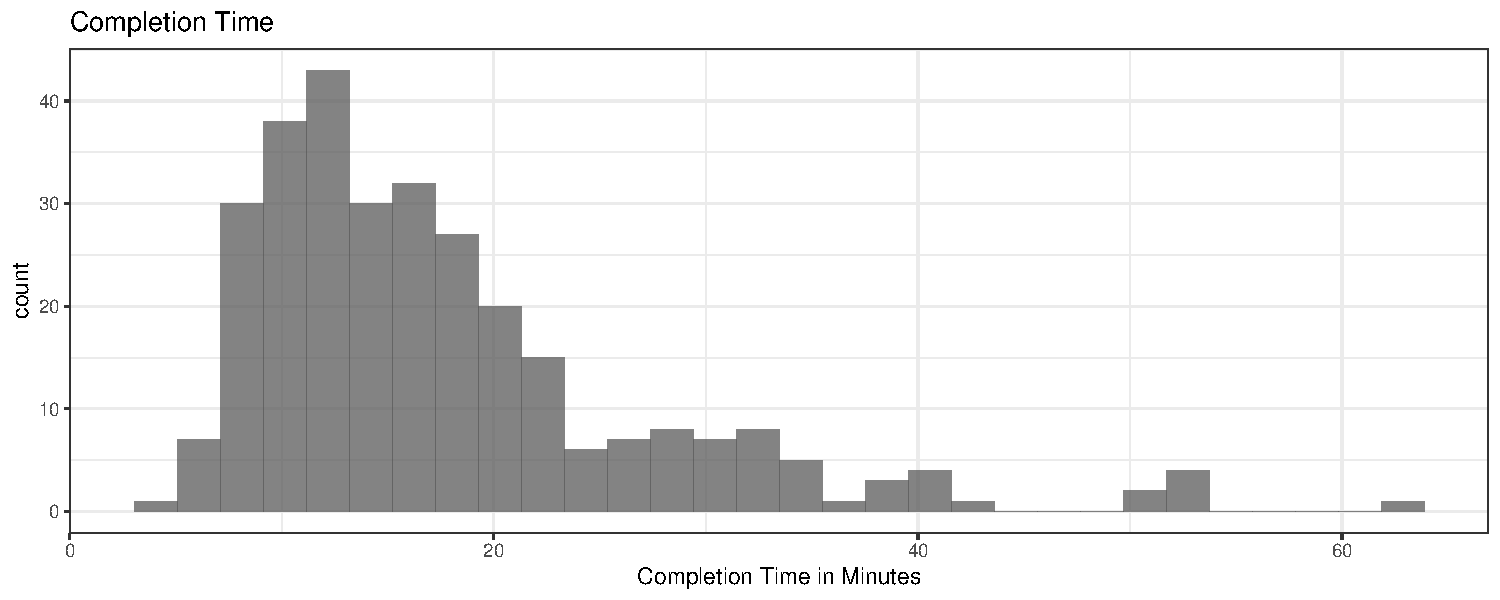
\includegraphics[width=\linewidth]{thesis_files/figure-latex/completiontime2-1} 

}

\caption{Prolific Completion Time}\label{fig:completiontime2}
\end{figure}

\hypertarget{results-1}{%
\section{Results}\label{results-1}}

\hypertarget{participants-1}{%
\subsection{Participants}\label{participants-1}}

\begin{figure}

{\centering 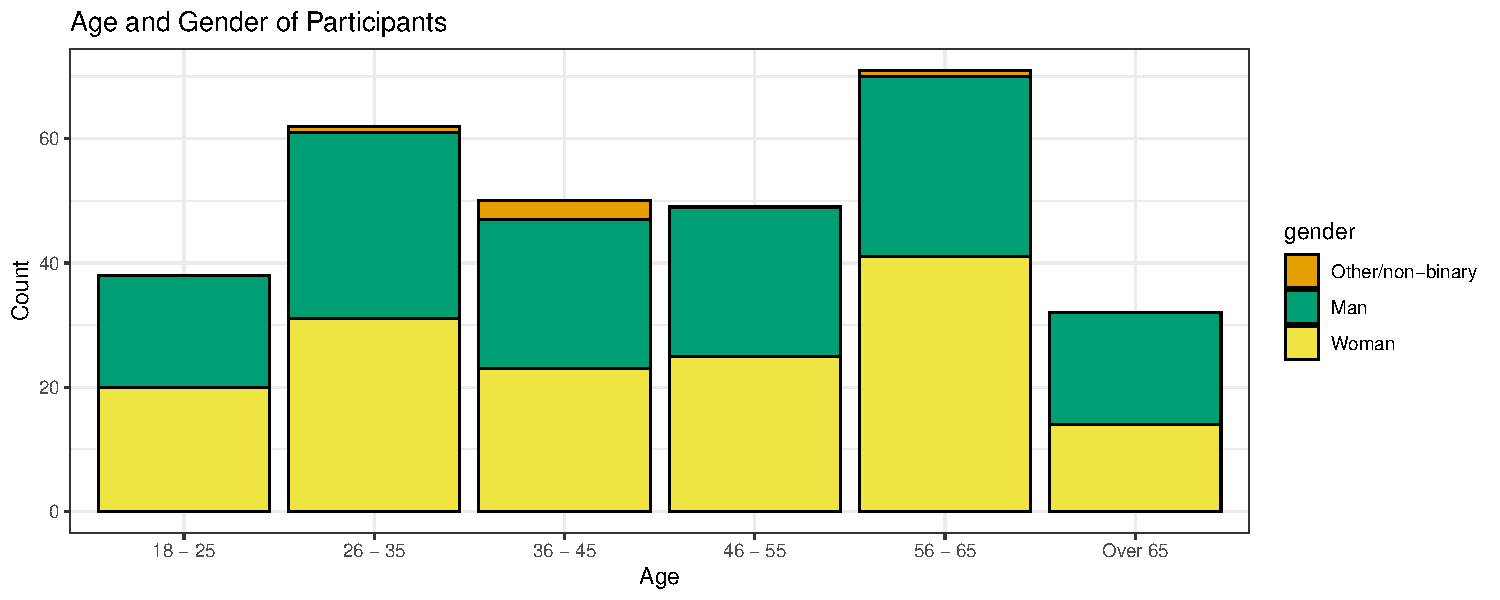
\includegraphics[width=\linewidth]{thesis_files/figure-latex/demographics2-1} 

}

\caption{Demographic Information}\label{fig:demographics2}
\end{figure}

Of the 302 surveys completed, 143 participants were men, 154 participants were women, and 5 participants identified as other or non-binary.
The median age category was 46 - 55.
Age and gender are shown in Figure \ref{fig:demographics2}.
Individuals were asked a single attention check question with regards to the caliber of gun used in the attempted robbery.
298 participants passed the attention check, meaning that only 4 participants failed the attention check, and will not be included in the analysis.
There were 147 participants in the identification condition and 151 participants in the elimination condition who passed the attention check.
We adjusted the probability of receiving each condition throughout the survey to ensure \svp{the number of participants across} categories \svp{was} relatively equal.

\hypertarget{questions-from-study-1}{%
\subsection{Questions from Study 1}\label{questions-from-study-1}}

There were some procedural changes made to this study compared to the original study that may influence results: namely, more detailed cross examination and the inclusion of jury instructions.
\svp{These changes were made in order to reduce scale compression by providing a stronger defense and emphasizing the role of the expert witness as providing opinions.}
Another significant difference between the two studies is the time that has passed between the two studies.
The first study was conducted in July 2022, while this study was conducted in January 2024.
In this time, notoriety of firearms evidence has not remained the same - in this response study, a participant commented that they had recently read an article about the unreliability of firearms evidence:

\begin{quote}
\authorcol{"Recently I have seen an article about a court decision that testimony about fired bullet comparisons have been shown to be unreliable.  At least some convictions in that state based upon fired bullet comparisons have been overturned.  I did not use that information in this case." - Elimination}
\end{quote}

\svp{This is in part due to a number of high-profile court cases in jurisdictions around the country which have limited the presentation of firearms evidence or how expert witnesses may present evidence to ensure that witnesses do not overstate the scientific value of firearms comparisons.}

More widespread criticism of firearms examination may lead to lower feelings of reliability.

In both studies, participants are asked if they would choose to convict, given the ``beyond a reasonable doubt'' threshold.
In this study, 54.42\% (or 80 out of 147) individuals who received the identification condition chose to convict, while 3.97\% (or 6 out of 151) participants who received the elimination condition chose to convict.
The conviction percentage for the identification condition in this study is slightly lower than the comparable condition in the original study (without the use of the algorithm and images): 61.82\% (or 34 out of 55).
However, there is not a significant difference between studies (p-value 0.43).
None of the 49 individuals in the original study who received the elimination condition without the use of the algorithm or images chose to convict.

\begin{figure}

{\centering 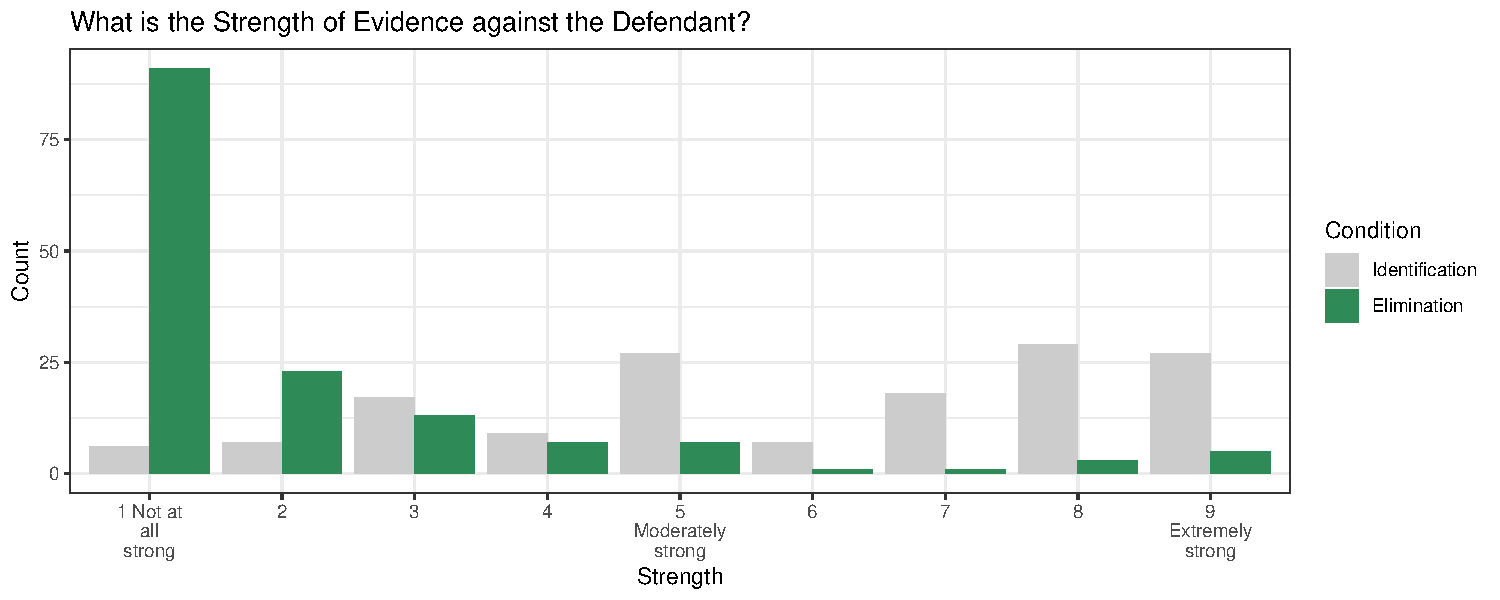
\includegraphics[width=\linewidth]{thesis_files/figure-latex/strength2-1} 

}

\caption{Microstudy Strength of Evidence}\label{fig:strength2}
\end{figure}

Figure \ref{fig:strength2} shows participant responses to the strength of evidence in this study.
\svp{Participants} in the elimination category tend to choose the smallest value for the strength of evidence (``Not at all strong''), while in the identification condition, individuals tend to distribute their views of the strength of evidence more evenly.
This graph resembles the strength of evidence results from the initial study, shown in Figure \ref{fig:strength}.
While not as dramatic as the scale compression for questions of reliability, credibility, and scientificity, the elimination results for strength of evidence do appear to show a scale limitation because individuals tended to overwhelmingly select the lowest category.

\begin{figure}

{\centering \includegraphics[width=\linewidth]{thesis_files/figure-latex/prob2-1} 

}

\caption{Probability Cole Committed Crime}\label{fig:prob2}
\end{figure}

Figure \ref{fig:prob2} \svp{shows participant-}selected probabilities that the defendant committed the crime.
For a single participant, their hidden probability selection was recorded incorrectly (carrying over a previous answer), I have removed this observation when performing analysis on the hidden probability scale.
As in the case of the strength of evidence, the graph resembles the probability graph found in the initial study (Figure \ref{fig:probalgorithm}), where there is a higher peak of extreme values for the elimination conditions than for the identification condition.
When using a t-test to compare the mean visible probabilities for the identification and elimination condition to those comparable conditions of the initial study, there is not a significant difference for the identification condition, but is a significant difference in the elimination condition (p-values of 0.15 and 0.01, respectively).
The estimated mean is higher in this follow up study (16.57\%) than the initial study (9.98\%) in the elimination condition.
For the identification condition, the estimated probabilities are 74.52\% for the follow-up study and 79.78\% for the initial study.
In this study, the density curves for when the probability was visible or hidden remain similar.

\hypertarget{new-study-questions}{%
\subsection{New Study Questions}\label{new-study-questions}}

In addition to asking participants if they would choose to convict, participants were also asked about their opinion of the guilt of the defendant.
In this case, 74.15\% (or 109 out of 147) individuals who received the identification condition thought the defendant was guilty, while 3.97\% (or 6 out of 151) participants who received the elimination condition thought the defendant was guilty.
Figure \ref{fig:opinionguilt} shows the comparison between the participant's decision to convict and their personal opinion.
Approximately half of the participant in the identification condition who chose not to convict thought the defendant was in fact guilty.
This indicates that participants have different thresholds for their personal opinion of guilt compared to the ``beyond a reasonable doubt'' threshold.
Of the 80 individuals who chose to convict in the identification condition, 5 participants thought the defendant was in fact innocent.
This discrepancy may be due to participants reversing the strength of the thresholds - they feel that the evidence is strong enough to convict, but are not wholly convinced.

\begin{figure}

{\centering \includegraphics[width=\linewidth]{thesis_files/figure-latex/opinionguilt-1} 

}

\caption{Comparison of opinions of guilt and choice to convict}\label{fig:opinionguilt}
\end{figure}

Figure \ref{fig:betting} indicates how much participants said they would be willing to bet that the defendant was either guilty or innocent, if provided with \$50.
If the participant thought the defendant was innocent, they were asked how much they would be willing to bet that the defendant was innocent, and vice versa.
This figure indicates that most people who thought Cole was innocent in the elimination condition were willing to bet the full amount (84 out of 141 participants).
It also appears that people tended to select values multiples of 5 (283 out of 298, with 8 additional individuals selecting 0).
\svp{In follow-up studies, we will attempt to assess this in a more symmetric manner by allowing participants to bet more than \$50; this should allow for a wider discrimination of the strength of participant opinion.}
Those in the identification condition selected less extreme values (for both those who thought the defendant was guilty and those who thought the defendant was innocent) than what is seen in those with the elimination condition who thought the defendant was innocent.
In this way, the betting response is similar both to the strength of evidence response and the probability of committing the crime response.

\begin{figure}

{\centering \includegraphics[width=\linewidth]{thesis_files/figure-latex/betting-1} 

}

\caption{If the researchers provided 50 dollars, how much would you be willing to bet?}\label{fig:betting}
\end{figure}

The remaining questions relate to the chance that the defendant committed the crime.
One question, shown in Figure \ref{fig:fixedlike}, allowed participants to select the chance that the defendant committed the crime from a multiple choice scale.
This scale does not provide a linear distance between intervals, but instead changes by multiples of 10 in the denominator (ex. one category is 1 in 10, and the next category is 1 in 100).
The exceptions are the endpoints, which are ``Impossible to be guilty'' and ``Certain to be guilty'', as well as the midpoint of 1 chance in 2.
In this case, the scale in the elimination condition does not encounter the ceiling or floor effect that has been seen in previous scales, as participants did not overwhelmingly select the lowest value.
Instead, participants are distributed mainly throughout the lower half of the scale, while those in the identification condition tended to be a little closer to the center.
In both cases, participants are not crowded into a small number of categories.
Thus, the multiple choice chance scale has less scale compression than seen previously in the other response types.
This wider distribution may be the result of decompressing the end points - individuals have a variety of values to select that reflect their judgement of a low probability that the defendant committed the crime, or a low strength of evidence.

\begin{figure}

{\centering \includegraphics[width=\linewidth]{thesis_files/figure-latex/fixedlike-1} 

}

\caption{Multiple Choice Chance}\label{fig:fixedlike}
\end{figure}

\begin{figure}

{\centering \includegraphics[width=\linewidth]{thesis_files/figure-latex/freelike-1} 

}

\caption{Free Response Chance}\label{fig:freelike}
\end{figure}

A final question asks individuals to provide a numerical chance that the defendant is either innocent or guilty, depending on the participants' choice (the question defaulted to chances of innocence, but participants had the option to switch the scale).
Their responses were limited so that the numerator was smaller than the denominator, resulting in a range of values from 0 to 1.
These results are shown in Figure \ref{fig:freelike}.
As seen in previous response types, in the case of the elimination condition, individuals gave small values for the chance that the defendant had in fact committed the crime, resulting in a sharp peak.
Alternatively, individuals were less extreme when they expressed their opinion as the chance that the defendant did not commit the crime in the elimination condition, even though the same sentiment is being expressed.
In the case of the identification condition, those who expressed their opinions as either guilt or innocence gave similar results, resulting in symmetry between the two distributions.
As shown in Figure \ref{fig:opinionchanceplot}, those who thought the defendant was innocent were more likely to favor inputting chance values in terms of innocence(0.6312849\%, or 113 out of 179), while those who thought the defendant was guilty were slightly less likely to express chance in terms of innocence (0.4621849\% expressed their beliefs in terms of innocence, or 55 out of 119).
This resulted in a significant difference between the two groups (\authorcol{Pearson's chi-squared test statistic} p-value of 0.006).

\begin{figure}

{\centering \includegraphics[width=\linewidth]{thesis_files/figure-latex/opinionchanceplot-1} 

}

\caption{Moasiac plot of participants who chose to express chance in terms of guilt or innocence, based on their opinion of the guilt of the defendant. The width of the bar corresponds to the number of participants per category.}\label{fig:opinionchanceplot}
\end{figure}

\hypertarget{scale-comparison}{%
\subsection{Scale Comparison}\label{scale-comparison}}

In addition to resolving scale compression, consistency across response types is another important aspect of this study.
If different question types result in responses that are inconsistent, it would be difficult to tell which questions truly capture the attitudes of the participants, in order to most accurately answer the research questions.
As mentioned in the Chapter \ref{litreview}, Thompson \& Newman (2015) suggest that individuals may struggle with the interpretation of likelihood scales, while chance scales were more consistent with Bayesian estimates.
Other scales, such as how much a participant is willing to bet, may be highly subjective - depending their personal feel for risk, and betting hypothetical money may have different results than betting real money.
Due to this potential difficulty in interpretation, response scales must be compared.
Schwarz (2010) \authorcol{indicate that order matters in partially-redundant questions, where participants may assume that later questions are asking about different facets than the initial question.}
Because individuals may be influenced by the order of the questions (such as choosing a numeric chance value that aligns with their multiple choice selection), the order was randomized and recorded \svp{so that we are averaging across any potential biasing effects due to question order}.

\begin{figure}

{\centering \includegraphics[width=\linewidth]{thesis_files/figure-latex/questorder-1} 

}

\caption{Order of Study Questions}\label{fig:questorder}
\end{figure}

Figure \ref{fig:questorder} \authorcol{depicts the order of the questions (the first three questions, conviction decision, comments on the defendant, and opinion of guilt, were not randomized).
The page on which each question appeared seems to be fairly random, with roughly equal proportions.}

\hypertarget{consistency-with-opinion-of-guilt}{%
\subsubsection{Consistency with Opinion of Guilt}\label{consistency-with-opinion-of-guilt}}

\begin{figure}

{\centering \includegraphics[width=\linewidth]{thesis_files/figure-latex/opinioncomp-1} 

}

\caption{Opinion of Guilt Consistency with Scales}\label{fig:opinioncomp}
\end{figure}

Perhaps the simplest question that we asked participants was whether or not they personally thought the defendant was guilty of committing the crime.
This opinion can provide a baseline for participant understanding of response questions.
If we set a threshold for opinion of guilt at a fifty-fifty chance (or 50\% probability of committing the crime), we can compare whether or not participant responses are within the expected range of their opinion of guilt, as shown in Figure \ref{fig:opinioncomp}.
This figure demonstrates that most individuals were consistent in their opinion of guilt and their selected values for the defendant committing the crime: meaning that if the participant thought the defendant was guilty, they selected at or more than a 50\% chance of guilt or a fifty-fifty chance, and vice versa.
This consistency is especially low for the numeric chance question, with 14.43\% of individuals providing inconsistent answers (compared to 4.7\%, 5.05\%, and 5.37\% for visible probability, hidden probability, and multiple choice chance, respectively).
Numeric chance can be broken into two categories, depending on if individuals chose to express numeric chance in terms of innocence or guilt.
Dividing along these lines results in 19.64\% of individuals providing inconsistent answers when expressing numeric chance of guilt in terms of innocence, and 7.69\% providing inconsistent answers when expressing chance in terms of guilt.
This demonstrates confusion in participants when expressing numeric chance in terms of innocence, while the consistency of numeric chance in terms of guilt is similar to that of the probability and multiple choice chance scales.
The numeric scale defaulted to chance of innocence, so it is possible that this scale reversal was overlooked by participants.

\hypertarget{numeric-and-multiple-choice-chance-comparison}{%
\subsubsection{Numeric and Multiple Choice Chance Comparison}\label{numeric-and-multiple-choice-chance-comparison}}

\begin{figure}

{\centering \includegraphics[width=\linewidth]{thesis_files/figure-latex/likecomp1-1} 

}

\caption{Chance of Guilt Comparison}\label{fig:likecomp1}
\end{figure}

Figure \ref{fig:likecomp1} shows the comparison of the multiple choice chance responses to the numeric chance responses, in the case that the participants chose to express the numeric chance in terms of guilt.
The red dots represent the actual value corresponding to their selection of the multiple choice chance (for example, the red dot for ``About 1 chance in 10'' is located at the y-value of 0.10).
This allows for comparison of the consistency between the multiple choice and the numeric scales.
For values of ``1 chance in 2'', ``About 1 chance in 10'', and ``About 9 chances in 10'', the responses seem fairly consistent - however, it is difficult to tell if these values are consistent for more extreme values, because they are compressed on the linear scale.

\begin{figure}

{\centering \includegraphics[width=\linewidth]{thesis_files/figure-latex/likecomp1scale-1} 

}

\caption{Guilt Chance Comparison Log 10 Scale}\label{fig:likecomp1scale}
\end{figure}

Figure \ref{fig:likecomp1scale} demonstrates the lower half of the multiple choice scale, when the x-axis is transformed by log 10.
The lines indicate the numerical equivalent to the multiple choice wording, including a black line for the ungraphed category of ``1 chance in 2 (fifty-fifty chance)''.
Based on this transformed scale, there is some consistency between participants' numeric chance choice and their multiple choice answer.
Numeric answers generally fall in the same area as their multiple choice selection.
However, many individuals did not show consistent choices between scales - particularly in the ``About 1 chance in 10,000'' condition, where several numerical choices would have better aligned with different selections in the multiple choice section, as demonstrated by the closeness of several observations to other multiple choice chance values.

\begin{figure}

{\centering \includegraphics[width=\linewidth]{thesis_files/figure-latex/likecomp1scalerev-1} 

}

\caption{Guilt Chance Comparison Log 10 Scale, where values were subtracted from 1}\label{fig:likecomp1scalerev}
\end{figure}

Figure \ref{fig:likecomp1scalerev} demonstrates the upper half of the multiple choice scale.
In order to visualize these compressed values, I subtracted the numerical chance selected by participants from 1 and used a log 10 transformation on the x-axis.
Thus, values can be interpreted as the chance that the defendant was innocent, even though participants chose to express their values in terms of guilt.
The lines indicate the numerical equivalent to the multiple choice wording, if expressed in terms of innocence.
For example, those selecting ``About 99 chances in 100'' of guilt would correspond to a value of 0.01 for the chance of innocence.
While those selecting ``About 9 chances in 10'' were fairly consistent with the expected value, there is a fair amount of inconsistency between participants' multiple choice selection and their numerical values for all other categories.
Those who selected ``Certain to be guilty'' tended to choose guilt values of 1 (or, alternatively, chance of innocence values of 0), as expected.
Other numerical values tended to cluster around 0.01 - 0.1 as the chance of innocence (individuals selected values between 0.9 and 0.99 in their numerical calculation of guilt).
For values aside from ``About 9 chances in 10'', this trend indicates that participants tended to provide numerical values of guilt that were lower than the values they indicated on the multiple choice scale.

\begin{figure}

{\centering \includegraphics[width=\linewidth]{thesis_files/figure-latex/likecomp2-1} 

}

\caption{Chance of Innocence Comparison}\label{fig:likecomp2}
\end{figure}

This same procedure can be repeated for those who thought the defendant was guilty, as shown in Figure \ref{fig:likecomp2}.
In this case, because individuals chose to supply the chance that the defendant did not commit the crime, I reversed the multiple choice chance indicators (the red circles) by subtracting the given value from 1 to correspond to the chance of innocence.
There appears to be some confusion on the question wording in this case, as demonstrated by numerous responses in the ``About 1 chance in 1,000'' and ``About 1 chance in 100'' categories that individuals assigned low chance values - indicating that individuals selected a low chance of innocence when given the numerical format, but a high chance of innocence when given the multiple choice question.
Most median numeric values on the left half of the multiple choice scale do not align with the translated value from the multiple choice scale.
The reduced consistency seen in these graphs may related to the change in the question wording, where the multiple choice question considers the chance of guilt, while their numeric chance considered the chance of innocence.
Most individuals who had inconsistent responses between the numeric and multiple choice chance question thought that the defendant was innocent, indicating that the multiple choice scale is more consistent with their beliefs than their numeric selections.

\begin{figure}

{\centering \includegraphics[width=\linewidth]{thesis_files/figure-latex/likecomp2scale-1} 

}

\caption{Innocence Chance Comparison Log 10 Scale, where values were subtracted from 1}\label{fig:likecomp2scale}
\end{figure}

This apparent confusion is reinforced in Figure \ref{fig:likecomp2scale}, displaying the values corresponding to the lower half of the multiple choice scale.
As in Figure \ref{fig:likecomp1scalerev}, I have reversed the numeric values so a log transformation can be used to better visualize the data.
While both graphs show inconsistency in responses, leading to a clustering of density distributions, in this case the effect is more severe.
The only multiple choice values that shows some consistency with the numeric counterpoints is ``About 1 chance in 10'' and ``Impossible that he is Guilty'', while for all other multiple choice options participants tended to provide a lower chance of numerical innocence than their multiple choice selection would indicate (shown by values further right on the scale).
In two cases, for those who selected ``About 1 chance in 100'' and ``About 1 chance in 1,000'' of guilt, the most popular category between ``About 1 chance in 10'' and ``About 1 chance in 2'', which does not align with their multiple choice selection.

\begin{figure}

{\centering \includegraphics[width=\linewidth]{thesis_files/figure-latex/likecomp2scalerev-1} 

}

\caption{Innocence Chance Comparison Log 10 Scale}\label{fig:likecomp2scalerev}
\end{figure}

Interestingly, this inconsistency did not hold as strongly for the upper part of the multiple choice chance scale, shown in Figure \ref{fig:likecomp2scalerev}.
Here, lines indicate the appropriate level chance of innocence corresponding to the multiple choice scale of guilt.
In this case, the bottom two categories (``About 9 out of 10'' and ``About 99 out of 100'') correspond quite well between the multiple choice answer and the numeric counterpart.
Although this consistency is not as present in the other categories, due to a larger variety of inputs, they are closer to the ballpark than what is shown in Figure \ref{fig:likecomp2scale}.
None of the individuals who selected ``Certain to be guilty'' on the multiple choice scale chose the corresponding 0 chance value of innocence, instead largely choosing values consistent with ``About 99 chances in 100''.

\begin{figure}

{\centering \includegraphics[width=\linewidth]{thesis_files/figure-latex/correctrangemosaic-1} 

}

\caption{Participants who selected the consistent range}\label{fig:correctrangemosaic}
\end{figure}

This inconsistency based on the scales is summarized in Figure \ref{fig:correctrangemosaic}.
Here, individuals were classified asn selecting the a numeric chance value in the consistent range if their multiple choice selection was the closest option for their numeric value.
Those who chose to express numeric choice in terms of innocence were less likely to input a value corresponding to their multiple choice selection (46.43\% consistent, or 78 out of 168 consistent for chance of innocence, and 67.69\% consistent, or 88 out of 130 consistent for chance of guilt).
This represents a significant difference in consistent ranges based on how participants chose to express the numeric chance (p-value: \ensuremath{4\times 10^{-4}}).
While only 67.69\% of those expressing numeric chance in terms of guilt selected the closest multiple choice answer to their numeric chance value, based on Figures \ref{fig:likecomp1scale} and \ref{fig:likecomp1scalerev}, many individuals were within the same region with their estimates, even if they could have chosen a better-fitting category.
Individuals who chose to express numeric chance in terms of innocence particularly struggled with the lower end of the multiple choice chance scale (from ``About 1 chance in 10,000'' to ``About 1 chance in 100''), corresponding to the higher end of the numeric chance scale.
Additionally, those who expressed numeric chance in terms of guilt struggled with two higher categories (``About 999 chances in 1,000'' and ``About 9,999 chances in 10,000'').

Overall, individuals tended to provide more consistent responses when evaluating numeric chance in terms of guilt instead of in terms of innocence.
While the upper parts of both innocent and guilty scales demonstrated less consistency than the lower parts of the numeric chance scales, the trends for those who expressed chance in terms of guilt more closely followed their multiple choice selections.

\hypertarget{probability-and-chance-scale-comparison}{%
\subsubsection{Probability and Chance Scale Comparison}\label{probability-and-chance-scale-comparison}}

\begin{figure}

{\centering \includegraphics[width=\linewidth]{thesis_files/figure-latex/likeprob-1} 

}

\caption{Probability and Chance Comparison}\label{fig:likeprob}
\end{figure}

The comparison of multiple choice chance and visible probability scales is shown in Figure \ref{fig:likeprob}.
In the case of the probabilities, individuals were only able to select integers between 0 and 100, meaning that this scale would be compressed for the more extreme values of the multiple choice chance scale (outside of the values of ``About 1 in 100'' and ``About 99 in 100'').
While there is some discrepancy between choice selection, particularly in participants who selected a lower chance that the defendant is guilty, responses seem to overall be consistent.
Median values in the boxplots indicate that the probability values tend toward the middle, pulling away from the extreme values on the probability scale that would correspond to their multiple choice chance answers.
However, on the whole both participants' selection in multiple choice answers and their probability selection correspond to their opinion of guilt.
The few individuals who selected high probability values but low multiple choice chance values expressed that their opinion was that the defendant was guilty.
This indicates that their selected probability value is more consistent with their opinion than the multiple choice chance value, indicating that these individuals may have found the use of the chance scale to be more confusing than the probability scale.

\begin{figure}

{\centering \includegraphics[width=\linewidth]{thesis_files/figure-latex/probchancescale1-1} 

}

\caption{Probability of Guilt Comparison to Multiple Choice Chance}\label{fig:probchancescale1}
\end{figure}

Figure \ref{fig:probchancescale1} compares the probability values to the participant's multiple choice chance decision.
Green indicates that participants selected the multiple choice value that is closest to their selected probability, while grey indicates that they could have selected a closer multiple choice value.
Overall, participant selections appear to be fairly consistent between scales, with some individuals tending towards less extreme values in the more extreme parts of the scale.
If participants were consistent in their choices of chance category and visible probability, we would expect that individuals selecting ``About 1 chance in 1,000'' or lower would exclusively select probability of guilt values of 1\% or 0\%.
While most individuals in the ``Impossible he is guilty'' category did select 0\%, this prediction does not hold true for the other categories.
In the case of ``About 1 chance in 10,000'' and ``About 1 chance in 1,000'', many participants selected values between 1\% and 5.5\%.
The same trend holds true for the upper portion of the scale - while individuals generally selected either 100\% when they selected that the defendant was ``Certain to be guilty'', some participants selected less extreme values than their multiple choice selection for categories for ``About 9,999 chances in 10,000'' and ``About 999 chances in 1,000''.
When scale values are more spread out, between ``About 1 chance in 100'' and ``About 99 chances in 100'', participant values on the probability scale tend to correspond with their multiple choice chance scale selection.
This demonstrates that this calibration issue mostly affects those who select extreme values.
While 50\% was the most popular (and default) value on the visible probability scale (selected by 33 participants), the next two most popular values are 0\% and 1\% (both selected by 21 participants).

\begin{figure}

{\centering \includegraphics[width=\linewidth]{thesis_files/figure-latex/correctprobmosaic-1} 

}

\caption{Participants who selected the consistent range between probability and multiple choice chance}\label{fig:correctprobmosaic}
\end{figure}

Results generally indicate consistent beliefs in guilt; by far most individuals who selected a multiple choice chance value corresponding to the defendant being more likely to be guilty than innocent selected a corresponding probability value in the same range (i.e.~less than a 50\% probability of being innocent), and vice versa.
However, the inconsistency in the scales is present in the form of magnitude: participants tended to select less extreme probability values than was indicated by their multiple choice chance selections.
In particular, individuals do well for values in the middle and at the endpoints, as shown in Figure \ref{fig:correctprobmosaic}, but they struggle with multiple choice values that are between the most extreme choices (0\% - 1\% and 99\% - 100\%). When comparing the multiple choice selection to visible probability, 59.73\% of individuals selected a visible probability value that corresponded to the range of their multiple choice selection.
This does not account for probability values that were similar, but would be better when placed in a different multiple choice category.
This percentage is lower than what was seen when comparing numeric chance of guilt to participants' multiple choice selection, which may be expected given the similar wording between the multiple choice and numeric chance categories.
However, the percentage of correspondence is higher than what was seen for participants who expressed numeric chance in terms of innocence.

\begin{figure}

{\centering \includegraphics[width=\linewidth]{thesis_files/figure-latex/likeprobcon-1} 

}

\caption{Probability and Chance Comparison}\label{fig:likeprobcon}
\end{figure}

Figure \ref{fig:likeprobcon} shows a comparison of the perceived probability that the defendant committed the crime compared to the perceived chance that the defendant is either innocent or guilty, when expressed on a continuous scale.
The plot lines would indicate a direct correspondence between chance value and probability.
Values are clustered near the corresponding corners of each plot.
This may be due to the compression on the probability scale - values of chance that are more extreme than 1 in 100 or 99 in 100 are represented with a single probability value.
Most responses that do not follow the line are below it when participants chose to express chance of innocence.
The clustering of low chance of innocence and low probability of guilt shown in the bottom left of the plot indicate participants who were confused about the chance scale - their opinion indicated that they thought the defendant was innocent, yet they assigned a low chance of innocence in the numerical scale.
The correlation between the probability and the chances of guilt is 0.91,
while the correlation between the probability and the chances of innocence is -0.75.
While there is a fairly strong correlation in the case of chances of guilt and probability, the correlation between the probability and the chances of innocence is weaker.
This may be a result of confusion in the scale reversal of the chance of innocence scale, while the chance of guilt \authorcol{regularly} corresponds with expressing the probability of guilt.

\hypertarget{evidence-strength-and-chance}{%
\subsubsection{Evidence Strength and Chance}\label{evidence-strength-and-chance}}

\begin{figure}

{\centering \includegraphics[width=\linewidth]{thesis_files/figure-latex/coordstrcat-1} 

}

\caption{Plots of perceived strength of evidence and categorical likelihood}\label{fig:coordstrcat}
\end{figure}

Figure \ref{fig:coordstrcat} shows the relationship between individuals' ratings of the strength of evidence, the categorical selection of the chance that the defendant committed the crime, \authorcol{and their assigned visible probability.}
While strength of evidence is on a 9-point Likert scale, the multiple choice chance scale has 11 values, giving participants more selection.
On the y-axis, lower values correspond to weaker strength of evidence and a lower chance of committing the crime, while higher values correspond to stronger strength of evidence and a higher chance of committing the crime.
In the case of the identification condition, there is a lack of equivalency between individuals' choice of strength of evidnece and the chance the defendant committed the crime, indicating that participants do not uniformly assign the same chances of committing the crime to the same strength of evidence.
Responses for the identification condition are also spread across many values on the scale, consistent with what we saw in the strength of evidence and multiple choice chance graphs, shown in Figures \ref{fig:strength2} and \ref{fig:fixedlike} respectively.
In the case of the elimination condition, most individuals chose the smallest level for the strength of evidence.
However, participant responses diverged in terms of the multiple choice chance that the defendant committed the crime: values corresponding to the lowest strength of evidence span four categories for the multiple choice chance, ranging from ``Impossible that he is guilty'' to ``About 1 chance in 100''.
The most popular categories corresponding to the weakest level of evidence strength were ``About 1 chance in 10,000'' and ``About 1 chance in 100''.
Similar to the relationship between probability and chance discussed in the previous section, this graphical comparison indicates compression on the strength of evidence scale.
The lowest strength of evidence category can be mapped to several different values for the chance that the defendant committed the crime.
\authorcol{Probability values in the elimination condition also converge upon lower values across several multiple choice chance categories.
In the identification condition, most participants tended to select higher values.
There is also a convergence to a probability of 50}\%.

\begin{figure}

{\centering \includegraphics[width=\linewidth]{thesis_files/figure-latex/convictlike-1} 

}

\caption{Multiple Choice Chance and Conviction Choice}\label{fig:convictlike}
\end{figure}

Figure \ref{fig:convictlike} depicts the results for our study comparing the chances that the defendant committed a crime to the decision to convict.
Participants cross the threshold of being more likely to convict when they select ``About 9 chances in 10'' in the identification condition, with roughly equal numbers above ``About 9 chances in 10'' in the elimination condition.
This indicates that participants set a threshold of ``beyond a reasonable doubt'' to be at ``About 9 chances in 10''.
These results are consistent with Thompson et al. (2013), who also found a threshold of about 9 chances in 10, where participants who selected 9 chances in 10 or a higher chance amount were more likely to select a guilty verdict, while those below 9 chances in 10 were more likely to select a not guilty verdict.

\begin{figure}

{\centering \includegraphics[width=\linewidth]{thesis_files/figure-latex/opinionlike-1} 

}

\caption{Multiple Choice Chance and Opinion of Guilt}\label{fig:opinionlike}
\end{figure}

Another threshold that we consider in this study is participants' personal feelings of the guilt of the defendant.
We would overall expect the threshold for this opinion to be lower than the ``beyond a reasonable doubt'' threshold used in their conviction decision.
Figure \ref{fig:opinionlike} demonstrates the relationship between the chance scale and the participant's opinion of the guilt of the defendant.
In this case, individuals generally thought the defendant committed the crime if they were above the ``fifty-fifty chance'' value for the identification condition, showing a lower threshold for their opinion of guilt than seen in Figure \ref{fig:convictlike}, when they were asked for their conviction choice.
Individuals who selected the ``fifty-fifty chance'' are fairly evenly split on their opinion of the guilt of the defendant in the identification condition.
This is to be expected when the participant believes that there is an approximately equal chance that the defendant committed the crime, but are asked to make a binary decision.

\hypertarget{hidden-and-visible-probability-comparison}{%
\subsubsection{Hidden and Visible Probability Comparison}\label{hidden-and-visible-probability-comparison}}

\begin{figure}

{\centering \includegraphics[width=\linewidth]{thesis_files/figure-latex/probcomp-1} 

}

\caption{Comparison of Probability Scales}\label{fig:probcomp}
\end{figure}

Figure \ref{fig:probcomp} shows the correspondence between the visible and hidden probabilities.
The values appear to be fairly 1:1.
In the visible probability scale, there is a slight trend of values clustering on multiples of 5 that is not present in the hidden probability scale.
For the identification condition, those who thought the defendant was guilty tended to select probability values above 50\%.
The correlation between the probabilities is 0.98, indicating a strong relationship between the hidden and visible scales.

\begin{figure}

{\centering \includegraphics[width=\linewidth]{thesis_files/figure-latex/probbet-1} 

}

\caption{Betting and Probability Comparison}\label{fig:probbet}
\end{figure}

Figure \ref{fig:probbet} compares the amount that individuals were willing to bet to their hidden probability that the defendant had/had not committed the crime.
Whether the participants were betting on the guilt or innocence of the defendant depended on their personal opinion of guilt - those who thought the defendant was guilty bet on the defendant's guilt, while those who thought the defendant was innocence bet on the defendant's innocence.
Values are clustered at two points.
For those who thought the defendant was innocent, they were willing to bet almost all of the \$50 and assigned a low probability to the defendant committing the crime.
For those who thought the defendant was guilty, they were also willing to bet almost all of the \$50, but assigned a high probability to the defendant committing the crime.
There is no clear pattern to individuals who fell outside of these two extreme points.
The correlation is 0.58 in the case that the participants were asked to bet on if the defendant committed the crime, and -0.57 when participants were asked to bet on if the defendant did not commit the crime.
These correlations are lower than both correlations between numeric chance and probability.
Based on the graph, this may indicate that both the probability scale and the betting scale suffer from compression in the most extreme values, with little correspondence on the remainder of the scale.

Mattijssen, Witteman, Berger, Brand, et al. (2020) compared likelihood and strength of evidence ratings from 10 examiners who regularly used likelihood scales.
While this sample size is rather small, they found that examiners tended to give higher verbal degrees of support than they should have, based on their likelihood ratio.
A similar effect can be investigated in the potential jurors of this study, when asked to rate the strength of evidence in the case as compared to their perceived probability that the defendant committed the crime.

Figure \ref{fig:strengthprob} shows the relationship between the strength of evidence compared to the probability that the defendant committed the crime.
In the identification condition, there is a generally increasing correspondence between the perceived strength of evidence and the participants' predicted probability that the defendant committed the crime.
This correspondence is less clear in the elimination condition, perhaps due to scale compression.

\begin{figure}

{\centering \includegraphics[width=\linewidth]{thesis_files/figure-latex/strengthprob-1} 

}

\caption{Strength of Evidence and Numerical Chance of Committing the Crime}\label{fig:strengthprob}
\end{figure}

\hypertarget{demographic-comparison}{%
\subsection{Demographic Comparison}\label{demographic-comparison}}

Demographic information, such as income, race, gender, and education level, was collected on the participants.
This demographic information can be compared with the participants' responses.

\hypertarget{income}{%
\subsubsection{Income}\label{income}}

Figure \ref{fig:probincome} explores a potential relationship between income and believed probability that the defendant committed the crime.
There does not appear to be a relationship between the two variables.

\begin{figure}

{\centering \includegraphics[width=\linewidth]{thesis_files/figure-latex/probincome-1} 

}

\caption{Income and Probability Comparison}\label{fig:probincome}
\end{figure}

Bases on Figure \ref{fig:convictsincome}, some individuals in the match condition chose to convict across all income levels.
There does not appear to be a clear trend between conviction choice and income.
Several income brackets chose to convict over the choice not to convict, but these brackets are spread throughout the scale.
In the case of the elimination condition, the individuals who did choose to convict came from different income brackets.

\begin{figure}

{\centering \includegraphics[width=\linewidth]{thesis_files/figure-latex/convictsincome-1} 

}

\caption{Income and Conviction Comparison}\label{fig:convictsincome}
\end{figure}

One may expect income to make a difference in how much individuals choose to bet on their opinion in the case, either in the amount of risk an individual is willing to take or in their desire to keep hypothetical money.
This does not appear to be the case, however, based on Figure \ref{fig:incomebet}.
As discussed earlier, many participants in the elimination condition were willing to bet the full amount that the defendant was innocent.
This is reflected across most income categories as well.
In the case of the identification condition, we saw earlier that participants were not as extreme in their bets as is seen in the elimination condition.
This trend is also reflected in the boxplots, with a fairly similar distribution of both the innocent and guilty bets across all income categories.

\begin{figure}

{\centering \includegraphics[width=\linewidth]{thesis_files/figure-latex/incomebet-1} 

}

\caption{Income and Betting Comparison}\label{fig:incomebet}
\end{figure}

\hypertarget{education}{%
\subsubsection{Education}\label{education}}

Figure \ref{fig:probeduc} shows the education level along with the participants' probability that the defendant committed the crime.
In this case, there does not appear to be a relationship between education level and probability, as the boxplots for probability are similarly distributed across education levels.

\begin{figure}

{\centering \includegraphics[width=\linewidth]{thesis_files/figure-latex/probeduc-1} 

}

\caption{Education Level and Probability Comparison}\label{fig:probeduc}
\end{figure}

Figure \ref{fig:convictseduc} shows the relationship between the decision to convict and education level.
As before, there doesn't appear to be much of a relationship between education level and conviction decision.
In the identification condition, individuals chose to convict across all educational categories.

\begin{figure}

{\centering \includegraphics[width=\linewidth]{thesis_files/figure-latex/convictseduc-1} 

}

\caption{Education and Conviction Comparison}\label{fig:convictseduc}
\end{figure}

Figure \ref{fig:educbet} shows the relationship between the betting and the education level.
There does not appear to be a trend between the education level and the amount that participants were willing to bet.
Based on these graphs, it does not appear that there is a relationship between education level and responses.

\begin{figure}

{\centering \includegraphics[width=\linewidth]{thesis_files/figure-latex/educbet-1} 

}

\caption{Education and Betting Comparison}\label{fig:educbet}
\end{figure}

\begin{figure}

{\centering \includegraphics[width=\linewidth]{thesis_files/figure-latex/educrange-1} 

}

\caption{Education and Consistent Numeric Chance Range}\label{fig:educrange}
\end{figure}

There also doesn't appear to be a relationship between individuals who select the corresponding range between multiple choice and numeric chance scales and education, as shown in Figure \ref{fig:educrange}.
This graphic demonstrates inconsistency in individuals choosing to express chance of innocence across the board.

\hypertarget{gun-comfort}{%
\subsubsection{Gun Comfort}\label{gun-comfort}}

Participants were asked to rate how comfortable they are with guns.
Figure \ref{fig:convictscomfort} shows the relationship between choice to convict and comfort with guns.
There does not appear to be a big trend in conviction rate.
However, it can be seen in the identification condition that those who were extremely uncomfortable with guns were more likely to convict, while those who were extremely comfortable with guns were less likely to convict.

\begin{figure}

{\centering \includegraphics[width=\linewidth]{thesis_files/figure-latex/convictscomfort-1} 

}

\caption{Gun Comfort and Conviction Comparison}\label{fig:convictscomfort}
\end{figure}

\hypertarget{notepad-analysis}{%
\subsection{Notepad Analysis}\label{notepad-analysis}}

While the notepad analysis for this study still needs to be conducted, analysis of preliminary results indicate that individuals were less likely to directly copy testimony compared to the first study.
This may be due to the change in format - the use of speech bubbles breaks up the text, which may prevent highlighting the entire page of testimony.
Due to this change, the length of the collocation may need to be shortened.
\svp{However, this change may encourage participants to only select relevant portions of the testimony, which would provide more insight from the collocation analysis.}

\hypertarget{note-cleaning}{%
\subsubsection{Note Cleaning}\label{note-cleaning}}

One complication in this dataset that was not present in the previous dataset was a missing page in the middle of participant notes.
\authorcol{All participants had 14 pages of notes, aside from those who did not complete the survey.
However, page numbers go from 4 to 18 - which should correspond to 15 pages of notes; though only one participant had a note page at both 4 and 18.
This person was missing a number for page 17, resulting in the skipped page.
In order to provide consistent notes for all participants, we shifted the page numbering to start at 4 and end at 18 for all individuals.
Individuals having the same number of pages in their note pads indicates that the notes were likely recorded correctly, but there was an issue with the page counter.
We hypothesize that this may occur when participants click the "Next" page button multiple times due to a delay in the webpage loading.}
In this case, based on slight modifications from the sequential cleaning functions mentioned in Chapter \ref{textcolor}, the algorithm uses the last known page of previous notes for data cleaning.

In this study, 198 individuals used the notepad at least once, resulting in 2413 pages of uncleaned notes.
After data cleaning, there were 807 pages of notes, from 197 individuals.
The one individual present in the uncleaned notes that is absent in the cleaned dataset\svp{; this participant} only took notes on the description page prior to the trial transcript, so no transcript notes were present in their record.

\hypertarget{notepad-analysis-1}{%
\subsubsection{Notepad Analysis}\label{notepad-analysis-1}}

The full comment analysis transcript can be found at: \url{https://rachelesrogers.github.io/Presentations/Response\%20Type\%20Collocations/Response_Survey_Comment_Analysis.html}.
On the whole, the highlighting trends for this testimony are similar for that of the previous study (found in Chapter \ref{textcolor}).
The addition of speech bubbles instead of a transcript format is one major difference in the testimony format that may affect how much participants copy down directly.
This, along with approximately half the sample size, may account for the low values found in this transcript.

In this study, an additional questions were added to the cross examination regarding the subjectivity of the bullet comparison - namely, if another firearms examiner would use the same subjective criterion and reach the same conclusion.
A few of the participants wrote the firearms examiner's answer in their notepad, indicating that they paid attention to this question.
On the other hand, participants did not appear to copy down the final jury instructions given by the judge - regarding the treatment of the algorithm examiner as any other witness.
These changes represent two different types of information presentation.
The discussion of other examiner's comparisons is aimed to be more informational - it describes the process of firearms comparison.
The jury instructions, on the other hand, are aimed to be instructional - it it asks the reader to reflect on their own interpretation of the case.
While the lack of notes on jury instructions may indicate that participants did not find them to be relevant, it may also be a product of a more reflective and less informative piece of testimony.

\hypertarget{participant-comments}{%
\subsection{Participant Comments}\label{participant-comments}}

\authorcol{Participant comments are found in Appendix }\ref{select-comments}.
\authorcol{Individuals still indicated confusion about the partial testimony, and the firearms examiner testifying on behalf of the prosecution in the elimination condition:}

\begin{quote}
\authorcol{"were you trying to trick the reader? the firearms ex. said that the gun did not match." - Elimination}
\end{quote}

\begin{quote}
\authorcol{"Seems highly unlikely that the DA would take this case to trial with ZERO eyewitness identification, the gun seized was NOT the gun that was used in the robbery, and the traffic stop has some constitutional issues." - Elimination}
\end{quote}

\authorcol{While the visuals did not assist in clearing up this confusion, both the visuals and the notepad received generally positive reviews:}

\begin{quote}
\authorcol{"The visuals of the conversation really helped me to focus in on the study. Also GREAT idea with the notepad, i tend to forget important information when im overloaded and it helps to be able to jot things down. Thanks for the study, good luck with your research!" - Identification}
\end{quote}

\begin{quote}
\authorcol{"This was a very interesting study to take. I liked the graphics and I liked how the study moved forward easily and I understood everything asked of me. I had no problems taking the study and I really enjoyed taking this study." - Identification}
\end{quote}

\begin{quote}
\authorcol{"I like the graphics that help to create the feeling of a court of examination." - Identification}
\end{quote}

\authorcol{However, one individual indicated some technical issues, while another did not appreciate the format:}

\begin{quote}
\authorcol{"The display was uncomfortable. I had to keep enlarging, then reducing the screen size even though I had a 24 inch screen." - Identification}
\end{quote}

\begin{quote}
\authorcol{"The cartoon presentation of the testimony was childish. And where is any testimony about the defendant's guilty, i.e., alibi, alibi witnesses, etc." - Identification}
\end{quote}

\hypertarget{conclusion-2}{%
\section{Conclusion}\label{conclusion-2}}

Several things can be determined through this exploration of response type.
Probability and strength of evidence scales suffer from scale compression in the elimination condition, as can be seen by the proclivity of participants to overwhelmingly select near the most extreme values.
The amount that participants were willing to bet was also compressed around the maximum amount, with no clear relationship between probability and betting amount, aside from individuals generally betting near the maximum and selecting extreme values on the probability scale.
The chance scales were less compressed, with the best results from the multiple choice scale.
Individuals who chose to numerically express chance of innocence as opposed to chance of guilt demonstrated more of a tendency to reverse the scale.

\hypertarget{finalstudy}{%
\chapter{Conclusion}\label{finalstudy}}

The initial goal of this research was to investigate how a bullet matching algorithm or demonstrative evidence may affect juror perception of the courtroom evidence and procedure.
In the course of this investigation, we encountered two issues: testimony confusion and Likert scale compression.
In order to address these issues, we redesigned the study format to include cartoons and color-coded speech bubbles for clarity, and conducted a survey investigating response type.
We also designed a method for analyzing participant notes that were taken while reading through the testimony, to create a `heatmap' of areas of text that participants found to be important.
We also investigated various response types, and found that Likert and probability scales were not optimal for collecting data in this case - instead, multiple choice chance scales with non-linear intervals allowed for more spread in participants' answers.

These diverging avenues of investigation will again merged for a final study (in progress).
The new cartoon study format was well received by participants, the response type study indicates that phrasing questions in terms of chance (i.e.~``1 chance in 10 that\ldots{}'') reduced/eliminated(?) the scale compression seen in Likert scales, and the text analysis provides useful information about what participants found worth copying into their notes.
In consolidating the information learned from these sub-studies, we will return to the initial study with significant changes designed to assist in elucidating the relationship between the inclusion of an algorithm in courtroom testimony and juror perception.

\appendix

\hypertarget{testimony-transcripts}{%
\chapter{Testimony Transcripts}\label{testimony-transcripts}}

\hypertarget{firearm-examiner}{%
\section{Firearm Examiner}\label{firearm-examiner}}

Q: Please state your name.

A: John Smith

Q: Who do you work for? (\emph{State of {Arizona} vs. Eduardo {Vasquez} {Celaya}}, 2007, pp. 6--7)

A: The local police department

Q: What do you do for the police department? (\emph{State of {Arizona} vs. Eduardo {Vasquez} {Celaya}}, 2007, pp. 6--7)

A: I am a firearms examiner (\emph{State of {Arizona} vs. Eduardo {Vasquez} {Celaya}}, 2007, pp. 6--7)

Q: How long have you been doing that? (\emph{State of {Arizona} vs. Eduardo {Vasquez} {Celaya}}, 2007, pp. 6--7)

A: X amount of years

Q: What is a firearms examiner? (\emph{State of {Arizona} vs. Eduardo {Vasquez} {Celaya}}, 2007, pp. 6--7)

A: A firearms examiner is someone who looks at cartridge cases and bullets to determine whether they were fired in a particular firearm.

Q: What training is required to become a firearms examiner with the local police department? (\emph{State of {Arizona} vs. Eduardo {Vasquez} {Celaya}}, 2007, pp. 6--7)

A: I received my bachelor's degree in forensic science and in X year I transferred to the crime lab from the crime scene unit. (\emph{State of {Arizona} vs. Eduardo {Vasquez} {Celaya}}, 2007, pp. 6--7)
I underwent a two-year training program, which was supervised by experienced firearms examiners (\emph{State of {Florida} vs. Sheppard {Jr.}}, 2012, pp. 798--799);
I've toured manufacturing facilities and saw how firearms and ammunition were produced; and I've attended several national and regional meetings of firearms examiners.(\emph{State of {Arizona} vs. Eduardo {Vasquez} {Celaya}}, 2007, pp. 6--7)

Q: And during the course of your career, were you tested in proficiency to make sure.. you were still conducting appropriate examinations? (\emph{State of {Florida} vs. Sheppard {Jr.}}, 2012, pp. 798--799)

A: Yes. I have undergone annual proficiency examinations.(\emph{State of {Florida} vs. Sheppard {Jr.}}, 2012, pp. 798--799)

Q: Is the local police department lab accredited? (\emph{State of {Arizona} vs. Eduardo {Vasquez} {Celaya}}, 2007, pp. 6--7)

A: Yes, it is accredited by ASCLID/LAB (\emph{State of {Arizona} vs. Eduardo {Vasquez} {Celaya}}, 2007, pp. 6--7)

Q: And in addition to what you just told us, do you have other qualifications? (\emph{The {People} of the {State} of {Illinois} v. Eugene {Banks}, et. al}, n.d., p. 2)

A: Yes, I do.(\emph{The {People} of the {State} of {Illinois} v. Eugene {Banks}, et. al}, n.d., p. 2)

Q: Can you tell us what those are? (\emph{The {People} of the {State} of {Illinois} v. Eugene {Banks}, et. al}, n.d., p. 2)

A: Yes. I received training in the use of a bullet matching algorithm.
This is an algorithm that evaluates the characteristics of two fired bullets, in order to produce a score for the similarity of the bullets, where more similar bullets are more likely to have been fired from the same gun.
I attended a workshop on the algorithm on {[}DATE{]}, held by CSAFE -- Center for Statistics and Applications in Forensic Evidence.
This involved use of the algorithm alongside my personal judgement.
I found that my conclusion was reflected in the similarity score produced by the algorithm in all \#\# cases.

Q: Where does the bullet matching algorithm come from? (\emph{The {People} of the {State} of {Michigan} v. Andrew {Mack} {Johnson}, {Jr.}}, 2018, p. 5)

A: It was created by \_\_\_\_\_. (\emph{The {People} of the {State} of {Michigan} v. Andrew {Mack} {Johnson}, {Jr.}}, 2018, p. 5)

Q: How long has the state police been using the bullet matching algorithm? (\emph{The {People} of the {State} of {Michigan} v. Andrew {Mack} {Johnson}, {Jr.}}, 2018, p. 5)

A: They have been using it since \#\#\#.

Q: Have you testified in court previously regarding the bullet matching algorithm? (\emph{The {People} of the {State} of {Michigan} v. Andrew {Mack} {Johnson}, {Jr.}}, 2018, p. 5)

A: Yes, I have, approximately \#\# times. (\emph{The {People} of the {State} of {Michigan} v. Andrew {Mack} {Johnson}, {Jr.}}, 2018, p. 5)

Q: Have you, as a firearms examiner, have you testified about opinions, given your opinion about the results of your testing? (\emph{The {People} of the {State} of {Michigan} v. Andrew {Mack} {Johnson}, {Jr.}}, 2018, p. 5)

A: Yes, I have. (\emph{The {People} of the {State} of {Michigan} v. Andrew {Mack} {Johnson}, {Jr.}}, 2018, p. 5)

Prosecution: Your Honor, at this time I would ask that XXX be qualified as an expert in the field of firearms identification subject to cross examination. (\emph{The {People} of the {State} of {Illinois} v. Eugene {Banks}, et. al}, n.d., p. 4)

Court: Any cross on their credentials? (\emph{The {People} of the {State} of {Illinois} v. Eugene {Banks}, et. al}, n.d., p. 4)

Defense: No, Your Honor (\emph{The {People} of the {State} of {Illinois} v. Eugene {Banks}, et. al}, n.d., p. 4)

Court: This witness is an expert in the area of firearms identification.
They can testify to their opinions as well as facts.
Go ahead.(\emph{The {People} of the {State} of {Illinois} v. Eugene {Banks}, et. al}, n.d., p. 4)

Q: What work did you do on this case? (\emph{State of {Arizona} vs. Eduardo {Vasquez} {Celaya}}, 2007, p. 8)

A: I was asked to compare a bullet from the crime scene to a test fire from XX gun.(\emph{State of {Arizona} vs. Eduardo {Vasquez} {Celaya}}, 2007, p. 8)

Q: Did you examine how many lands and grooves the bullet had? (\emph{State of {Arizona} vs. Eduardo {Vasquez} {Celaya}}, 2007, pp. 17--18)

A: Yes. (\emph{State of {Arizona} vs. Eduardo {Vasquez} {Celaya}}, 2007, pp. 17--18)

Q: Can you explain for the jury what that means? (\emph{State of {Arizona} vs. Eduardo {Vasquez} {Celaya}}, 2007, pp. 17--18)

A: Yes\ldots{} In the interior of a barrel there are raised portions called lands and depressed areas called grooves.
When a bullet passes down the barrel, a bullet will spin and that gives it stability and accuracy over a distance.
Those raised areas are designed by the manufacturer.
They're cut into the barrel.
And each particular file has a different combination of lands and grooves.
But essentially what those lands do will grip a bullet and spin it and as that bullet passes down the barrel, it scratches the random imperfections of that barrel into the bullet.(\emph{State of {Arizona} vs. Eduardo {Vasquez} {Celaya}}, 2007, pp. 17--18)

Q: Now, for these bullets, you counted up the lands and grooves and determined the direction of the twist, correct? (\emph{State of {Arizona} vs. Eduardo {Vasquez} {Celaya}}, 2007, pp. 17--18)

A: Yes. This bullet had six lands. And the interior of the barrel, the barrel will either twist right or it will twist left.
And this particular case, the barrel twists right.
And you can see that by looking at the bullet.
If you look at the base of the bullet, either it goes to the left or goes to the right.(\emph{State of {Arizona} vs. Eduardo {Vasquez} {Celaya}}, 2007, pp. 17--18)

---Test-fired bullets admitted into evidence---

Q: Can you describe the process of obtaining these test-fired bullets?

A: The test-fired bullets came from a test fire of XX gun.

Q: You mentioned test firings, can you explain what that means? (\emph{The {People} of the {State} of {Illinois} v. Eugene {Banks}, et. al}, n.d., p. 6)

A: In test firing first what I would do is make sure the firearm is safe to actually test fire.
Then I would use lab ammunition and I would test fire it, meaning that I'm creating a fired bullet.
Typically you do two at a time.
That way you have a fired bullet to compare to another fired bullet. (\emph{The {People} of the {State} of {Illinois} v. Eugene {Banks}, et. al}, n.d., p. 6)

Q: Would you then have taken the test firings you created and did you compare those test firings to the fired evidence that you had also received? (\emph{The {People} of the {State} of {Illinois} v. Eugene {Banks}, et. al}, n.d., p. 6)

A: Yes. First what I would do is compare my test shot to test shot.
I'm looking for a detailed microscopic pattern.
Once I have done that then I would compare it to the fired evidence.(\emph{The {People} of the {State} of {Illinois} v. Eugene {Banks}, et. al}, n.d., p. 6)

Q: And how about the number of lands and direction of twist for the test fires? (\emph{State of {Arizona} vs. Eduardo {Vasquez} {Celaya}}, 2007, pp. 19--20)

A: It also had six lands, and twisted to the right (\emph{State of {Arizona} vs. Eduardo {Vasquez} {Celaya}}, 2007, pp. 19--20)

Q: Okay. Now, did you compare the test-fired bullets to the fired evidence under the comparison microscope? (\emph{State of {Arizona} vs. Eduardo {Vasquez} {Celaya}}, 2007, pp. 19--20)

A: Yes, I did. (\emph{State of {Arizona} vs. Eduardo {Vasquez} {Celaya}}, 2007, pp. 19--20)

Q: What is your conclusion? (\emph{State of {Arizona} vs. Eduardo {Vasquez} {Celaya}}, 2007, pp. 19--20)

A: I found that there were sufficient individualizing characteristics to conclude that the two bullets were fired from the same barrel.

Q: How were you able to conclude that? (\emph{State of {Arizona} vs. Eduardo {Vasquez} {Celaya}}, 2007, pp. 19--20)

A: I placed them under the comparison microscope, and I roll the bullet around 'til I can see the agreement in a particular area, unique surface contour that has sufficient agreement.
At that point, when I've seen that, I start to rotate the bullets around and I look at all the different lands and grooves, impressions, for that unique detail.
When I can see those, that agreement on multiple areas of the bullet, I identify the bullet as having sufficient agreement.(\emph{State of {Arizona} vs. Eduardo {Vasquez} {Celaya}}, 2007, pp. 19--20)

Q: Did you use an algorithm to compare these bullets as well?

A: Yes, I used the algorithm to compare the two test fires to each other.
I also used the algorithm to compare the better-marking test fire to the fired evidence that I received.

Q: Could you explain how this algorithm compares bullets?

A: The algorithm uses 3D measurements to make a comparison between the surface contours of each of the lands on each bullet.
These comparisons result in a match score between 0 and 1, where 1 indicates a clear match, and 0 indicates that there is not a match.
The bullet is aligned based on the maximum agreement between the lands, and the average match score for the lands is computed.
This average score gives an overall match score for the entire bullet.

Q: What was the match score between the two test-fired bullets?

A: The match score was 0.9-.

Q: What was the match score between the better-marked test fire bullet and the fired evidence?

A: The match score was 0.XX.

Q: What does this match score indicate about the bullets?

A: The match score indicates that there is substantial similarity between the two bullets, which suggests that they were most likely fired from the same barrel.

Q: Now, how many times have you compared bullets to determine if they were fired from the same gun? (\emph{State of {Arizona} vs. Eduardo {Vasquez} {Celaya}}, 2007, pp. 19--20)

A: I'd say thousands. (\emph{State of {Arizona} vs. Eduardo {Vasquez} {Celaya}}, 2007, pp. 19--20)

Q: And do you ever see two bullets that have agreement in every area of the bullet? (\emph{State of {Arizona} vs. Eduardo {Vasquez} {Celaya}}, 2007, pp. 19--20)

A: No.~
The firing process of a firearm is dynamic, kind of like a contained explosion.
When the firing pin hits the primer, which is basically the initiator, what gets it going, it will explode, bur the gun powder inside the casing, and the bullet will travel down the barrel, picking up the microscopic imperfections of the barrel, and the cartridge case will slam rearward against the support mechanism.
During that dynamic process, each time it happens, a bullet will be marked slightly differently from one to the next. (\emph{State of {Arizona} vs. Eduardo {Vasquez} {Celaya}}, 2007, pp. 19--20)

Q: When you reached a conclusion, did you write up a report? (\emph{State of {Arizona} vs. Eduardo {Vasquez} {Celaya}}, 2007, p. 23)

A: Yes, I did. (\emph{State of {Arizona} vs. Eduardo {Vasquez} {Celaya}}, 2007, p. 23)

Q: Is it the local police department's protocol to have somebody else who's a firearms tool mark examiner in your lab review that report, review your work, and determine if it's correct? (\emph{State of {Arizona} vs. Eduardo {Vasquez} {Celaya}}, 2007, p. 23)

A: Yes. (\emph{State of {Arizona} vs. Eduardo {Vasquez} {Celaya}}, 2007, p. 23)

Q: That's what we call peer review? (\emph{State of {Arizona} vs. Eduardo {Vasquez} {Celaya}}, 2007, p. 23)

A: Peer review, yes. (\emph{State of {Arizona} vs. Eduardo {Vasquez} {Celaya}}, 2007, p. 23)

Q: Thank you, no further questions. (\emph{State of {Arizona} vs. Eduardo {Vasquez} {Celaya}}, 2007, p. 40)

--Cross examination----

Q: Now, are you telling the jury today that in your opinion there's only one gun in the entire world that could have produced the markings that you saw on these bullets? (\emph{State of {Arizona} vs. Eduardo {Vasquez} {Celaya}}, 2007, p. 65)

A: I'm saying that the probability that the two markings were made by different sources is so small that it is negligible. (Office of Legal Policy, 2020, p. 2) (\emph{State of {Arizona} vs. Eduardo {Vasquez} {Celaya}}, 2007, p. 65)

Q: Exclusive to any other gun? (\emph{State of {Arizona} vs. Eduardo {Vasquez} {Celaya}}, 2007, p. 65)

A: I obviously haven't tested every other gun, but it is a practical impossibility. (\emph{State of {Arizona} vs. Eduardo {Vasquez} {Celaya}}, 2007, p. 65)

Q: That's your opinion. And your opinion, by the way, is subjective, right, and it's based on your experience? (\emph{State of {Arizona} vs. Eduardo {Vasquez} {Celaya}}, 2007, pp. 72--73)

A: Based on my training and experience, yes. (\emph{State of {Arizona} vs. Eduardo {Vasquez} {Celaya}}, 2007, pp. 72--73)

Q: Is there something fixed about the amount of what has to be found to constitute sufficient agreement? (\emph{{U.S.} Vs. {Harris}}, 2016, pp. 4459--4460)

A: No, there is not a fixed amount or a numerical value. (\emph{{U.S.} Vs. {Harris}}, 2016, pp. 4459--4460)

Q: How long did you say you've been trained in the bullet matching algorithm? (\emph{The {People} of the {State} of {Michigan} v. Andrew {Mack} {Johnson}, {Jr.}}, 2018, p. 19 - 21)

A: Since XXX (\emph{The {People} of the {State} of {Michigan} v. Andrew {Mack} {Johnson}, {Jr.}}, 2018, p. 19 - 21)

Q: Okay. So that's fairly new; is that fair to say? (\emph{The {People} of the {State} of {Michigan} v. Andrew {Mack} {Johnson}, {Jr.}}, 2018, p. 19 - 21)

A: It is still fairly new, yes. (\emph{The {People} of the {State} of {Michigan} v. Andrew {Mack} {Johnson}, {Jr.}}, 2018, p. 19 - 21)

Q: The software uses modeling; is that correct? (\emph{The {People} of the {State} of {Michigan} v. Andrew {Mack} {Johnson}, {Jr.}}, 2018, p. 19 - 21)

A: Yes, it does. (\emph{The {People} of the {State} of {Michigan} v. Andrew {Mack} {Johnson}, {Jr.}}, 2018, p. 19 - 21)

Q: You, personally, don't know the source code; is that correct? (\emph{The {People} of the {State} of {Michigan} v. Andrew {Mack} {Johnson}, {Jr.}}, 2018, p. 19 - 21)

A: That's correct.(\emph{The {People} of the {State} of {Michigan} v. Andrew {Mack} {Johnson}, {Jr.}}, 2018, p. 19 - 21)

Q: And, in fact, you, personally, would not be able to tell us the specific math that goes into this program; is that fair to say? (\emph{The {People} of the {State} of {Michigan} v. Andrew {Mack} {Johnson}, {Jr.}}, 2018, p. 19 - 21)

A: We did receive training on what the math is doing. (\emph{The {People} of the {State} of {Michigan} v. Andrew {Mack} {Johnson}, {Jr.}}, 2018, p. 19 - 21)

The Court: Terry Smith, the jury has asked me to forward this question to you. Answer if you're able.
To what percentage is the science accurate is the first question. And then I think the rest of that explanation of that question goes on to say, to determine that the bullets were fired from the same firearm, are you 100 percent sure? (\emph{State of {Arizona} vs. Eduardo {Vasquez} {Celaya}}, 2007, pp. 100--101)

A: My opinion, I am 100 percent sure that these bullets were fired from this firearm.
There is a published error rate for firearms examiners.
The positive identification is less than two percent.
I believe it's about 1.5 to 1.9. That's just a general number that's out there.(\emph{State of {Arizona} vs. Eduardo {Vasquez} {Celaya}}, 2007, pp. 100--101)
The false negative identification rate is less than three percent. (Chumbley et al., 2021)

\hypertarget{algorithm-expert}{%
\section{Algorithm Expert}\label{algorithm-expert}}

Inspired by \emph{State of {Arizona} vs. Eduardo {Vasquez} {Celaya}} (2007), \emph{The {People} of the {State} of {Illinois} v. Eugene {Banks}, et. al} (n.d.), \emph{The {People} of the {State} of {Michigan} v. Andrew {Mack} {Johnson}, {Jr.}} (2018), \emph{{U.S.} Vs. {Harris}} (2016), \emph{State of {Florida} vs. Sheppard {Jr.}} (2012), Hare et al. (2017), Vanderplas et al. (2020), and Perlin (2012). Should create citations by line as above.

Q: Please state your name.

A: Adrian/Avery Jones

Q: Who do you work for? (\emph{State of {Arizona} vs. Eduardo {Vasquez} {Celaya}}, 2007, pp. 6--7)

A: XXX place

Q: What is your current occupation?

A: XXX

Q: How long have you been doing that? (\emph{State of {Arizona} vs. Eduardo {Vasquez} {Celaya}}, 2007, pp. 6--7)

A: X amount of years

Q: What training is required to hold this occupation? (\emph{State of {Arizona} vs. Eduardo {Vasquez} {Celaya}}, 2007, pp. 6--7)

A: I have a Ph.D.~in XX, and have spent X time developing the bullet matching algorithm algorithms.
I have spent X years collaborating with firearms examiners during the development and rollout of this algorithm.

Q: Are you familiar with the bullet matching algorithm?

A: Yes. I was involved in the development of the algorithm.

Prosecution: Your Honor, at this time I would ask that XXX be qualified as an expert in the bullet matching algorithm subject to cross examination.
Court: Any cross on their credentials? (\emph{The {People} of the {State} of {Illinois} v. Eugene {Banks}, et. al}, n.d., p. 4)

Defense: No, Your Honor (\emph{The {People} of the {State} of {Illinois} v. Eugene {Banks}, et. al}, n.d., p. 4)

Court: This witness is an expert in the area of the bullet matching algorithm. They can testify to their opinions as well as facts. (\emph{The {People} of the {State} of {Illinois} v. Eugene {Banks}, et. al}, n.d., p. 4)

Q: How many times have you testified regarding this bullet matching algorithm?

A: XX times.

Q: Could you describe how this bullet matching algorithm compares bullets?

A: Yes. For certain types of guns, the barrel will have lands and grooves, known as rifling.
This rifling spins the bullet in order to make its trajectory more stable. Due to the manufacturing process, this rifling can produce identifiable markings on the bullet, based on random differences between barrels.
Because of these random imperfections, the striation marks left on bullets can be compared in order to determine if it is likely that they were fired from the same gun.

(Description based on Hare et al. (2017))
The first step is to determine where the lands on the bullet are located.
These lands will be the sunken area that contains the striation marks between the smoother grooves.
3D scans are then taken for each land, and the `shoulders', or area transitioning from the land to the groove, is excluded from the analysis.

Next, a stable area of the 3D scan containing the striations is selected, and a cross-section of this area is used to show the striations along with the topology of the region.
A smoothing function is applied to remove some of the imaging noise from the 3D scan, leaving the striae intact.
A second smooth is subtracted from the striations in order to remove the curvature of the region, leaving only the striae -- this is what we call a signature.
The signature for the two bullets being compared are aligned such that the best fit between the two signatures is achieved.
The striation marks between the two signatures are then compared by evaluating how many of the high points and low points correspond.
The algorithm can calculate the number of consecutively matching striations (CMS), or consecutively matching high points and low points -- these are features used directly by some examiners to characterize the strength of a match.
It also calculates the cross correlation between the two signatures, which is a numerical measure of the similarity between the two lands ranging between --1 and 1.

These traits are combined using what is known as a random forest.
Each forest is composed of decision trees, which use a subset of the observed values in order to make a decision about whether or not the bullets constitute a match.
The other observations are held out in order to determine an error rate.
When the random forest makes a prediction, each decision tree ``votes'', producing a numerical value between 0 and 1 corresponding to the percentage of trees which evaluate the features as being sufficiently similar to have come from the same source.

Q: Have you tested this algorithm?

A: Yes.
This algorithm was tested and validated on a number of different test sets of bullet scans.
It was found that, as long as there are sufficient marks on the bullet, the algorithm could successfully distinguish between bullets fired by the same gun and those fired from different guns.
Examiners' visual comparisons are also limited by the presence or absence of individualizing marks.
Two test sets were using consecutively rifled barrels, which should be the most difficult to assess, and it was shown that the algorithm could distinguish between the bullets fired from two separate guns with complete accuracy. (Vanderplas et al., 2020)

Q: Can this algorithm be used on XX bullets fired from an XX firearm, such as the firearm in question for this case?
(Discussion of limitations (\emph{The {People} of the {State} of {Michigan} v. Andrew {Mack} {Johnson}, {Jr.}}, 2018, p. 11))

A: Yes, this algorithm can be used on these types of bullets, given that this type of firearm marks well.

Q: Has this algorithm been published? (Perlin (2012) for importance of publication)

A: Yes. The algorithm and its process has been discussed in peer reviewed journals such as Law, Probability, and Risk, The Annals of Applied Statistics, and Forensic Science International.
The algorithm is also open source, which means that the full source code, documentation, and numerical weights are available online for anyone to examine.

--Cross examination----

Q: How long has the bullet matching algorithm been used in court cases? (\emph{The {People} of the {State} of {Michigan} v. Andrew {Mack} {Johnson}, {Jr.}}, 2018, p. 19 - 21)

A: Since XXX

Q: Okay. So that's fairly new; is that fair to say? (\emph{The {People} of the {State} of {Michigan} v. Andrew {Mack} {Johnson}, {Jr.}}, 2018, p. 19 - 21)

A: It is still fairly new, yes. (\emph{The {People} of the {State} of {Michigan} v. Andrew {Mack} {Johnson}, {Jr.}}, 2018, p. 19 - 21)

Q: This algorithm requires some decision making on the part of the operator, such as how much the signature is smoothed and what part of the bullets are inputted into the system, correct? (subjective aspects (\emph{The {People} of the {State} of {Michigan} v. Andrew {Mack} {Johnson}, {Jr.}}, 2018, p. 21))

A: Yes, there are certain parameters which must be specified, but the system defaults are usually sufficient and have been validated with a number of different firearms and ammunition types.
There are also operating protocols for determining which parts of the bullet are scanned, so while this process is manual, there are clear criteria and the associated variability from scanning is well understood, and published in Forensic Science International.

Q: Can this algorithm be applied to all bullets? (gun specific/issues with damaged bullets)

A: No, the algorithm only works on traditionally rifled bullets which are largely undamaged.
The algorithm has not been validated to work on seriously damaged or fragmented bullets.

\hypertarget{study-2-changes}{%
\chapter{Study 2 Changes}\label{study-2-changes}}

\hypertarget{cautions-against-expert-witnesses}{%
\section{Cautions Against Expert Witnesses}\label{cautions-against-expert-witnesses}}

\hypertarget{jury-instructions}{%
\subsection{Jury Instructions}\label{jury-instructions}}

You have heard testimony from Terry Smith and Adrian Jones who have testified to opinions and the reasons for their opinions. This opinion testimony is allowed because of the education or experience of this witness.
Such opinion testimony should be judged like any other testimony.
You may accept or reject it, and give it as much weight as you think it deserves, considering the witness's education and experience, the reasons given for the opinion, and all the other evidence in the case. (United States Courts for the Ninth Circuit, 2019)

\hypertarget{opinion-witness}{%
\subsection{Opinion Witness}\label{opinion-witness}}

United States Courts for the Ninth Circuit (2019) suggests that witnesses should not be qualified as experts, as it may cause the jury to place undue weight in their testimony. Instead, Richey (1994) implements the term ``opinion witness'' in the place of ``expert witness''. This practice has been adopted in our revised testimony, when qualifying the witness based on experience and education.

\hypertarget{cross-examination}{%
\subsection{Cross Examination}\label{cross-examination}}

The strength of evidence (``the probability that the two markings were made by different sources is so small that it is negligible'') was moved from the cross examination to the direct examination, since this strength of evidnece should be introduced by the prosecution. Additional testimony regarding subjectivity was added to the cross examination as well, from (\emph{{U.S.} Vs. {Harris}}, 2016, p. 54):

Q: You have a criterion in you head, a subjective criterion, of what will constitute an identification. Is that correct?

A: Yes.

Q: All right. If we brought three more people in, would their subjective criterion in their head be identical to yours?

A: They would look for that same sufficient agreement. However, based on their training and experience on difficult comparisons, they may or may not come to the same decision.

Q: Right. But they also could reach the same decision but have a different subjective criterion than you. Is that fair?

A: They may, possibly. I don't know. I can't speak for other examiners.

Additional testimony was also added to address the distinction between evidence that the gun was at the crime scene, and evidence that Cole was at the crime scene (\emph{State of {Florida} vs. Sheppard {Jr.}}, 2012, p. 831):

Q: You can't tell us anything about who shot the firearm, correct?

A: That is correct.

\hypertarget{clarifying-sides}{%
\section{Clarifying Sides}\label{clarifying-sides}}

To make sure individuals are clear on who the firearms examiner is testifying for, testimony was added related to the calling and the swearing in of the witness. The testimony below is from \emph{The {People} of the {State} of {Michigan} v. Andrew {Mack} {Johnson}, {Jr.}} (2018).

Court: Your next witness, please.

Prosecution: The People would call John Smith.

Court: Hello.

Smith: Hi

Court: Would you raise your right hand for me? Do you sear the testimony you're about to give will be the truth, the whole truth, nothing but the truth, under penalty of perjury?

Smith: I do.

Court: Please be seated. State your full name for the record and spell your last name.

Witness: My name in John Smith, last name S-m-i-t-h

\hypertarget{images}{%
\section{Images}\label{images}}

In order to clarify the speakers in the testimony and create a more engaging environment, we implemented character drawings (by Richy Meleus) to represent various actors that may be present in the courtroom. These characters' faces and clothing are largely exchangeable, allowing for a large combination of clothing and characteristics.

\includegraphics[width=\linewidth]{thesis_files/figure-latex/demo_evidence-1}

\includegraphics[width=\linewidth]{images/Jury}

These images were placed in their respective speech bubbles in order to indicate the speaker, with color coding to indicate which side witnesses were testifying for: the prosecution's side had warmer colors, the defense had cooler colors, and the judge was a neutral grey.

\includegraphics[width=\linewidth]{images/Study2_Screenshot}
\includegraphics[width=\linewidth]{images/Study2_Screenshot2}

\hypertarget{select-comments}{%
\chapter{Select Comments}\label{select-comments}}

\hypertarget{initial-study}{%
\section{Initial Study}\label{initial-study}}

``Even if it seems like Richard Cole's gun is the same gun fired in the store, there is not enough (or any) evidence that Richard Cole was the one to fire the gun, so he cannot reasonably be convicted.''

``The 1.5\% error rate does seem sort of high, but at the same time it seems extremely unlikely that two guns that leave such similar bullet markings would be found in the general area of the crime.''

``Very difficult for juror to understand and remember the scientific evidence.''

``I'm not sure why the prosecution would have even called that witness because they basically said there was no conclusive bullet evidence''

``I think it's interesting there is not any evidence identifying the suspect from the witness or cameras. Makes it hard to make an accurate judgement, especially when the gun was obtained through a routine violation.''

``I'm wondering why testimony had to discuss details of the ML algorithm? When they use a microscope to examine evidence, does the examiner have to explain the optics of microscopes?''

``It seems likely that it was the gun but I'd love to have a witness who was skeptical of this stuff. But even if it's the gun, no evidence it was defendent who used it. I'm worried this is junk science but I don't know enough to ahve more than a lingering doubt.''

``Firearm evidence seems a lot like hair evidence which was debunked but I don't know that to be fact. From what was stated in this testimony, it seems to be mostly reliable but I wouldn't say it is strongly scientific.''

``Was interesting. I was very surprised that with today's technology, a fired bullet could still be labeled inconclusive.''

``Richard Cole has been victimized by the court system in this case. The seizure of his firearm - absent any other evidence - was most probably illegal. Police cannot be allowed to simply confiscate every legally owned gun they come across in case it was used to commit a crime.''

``I would trust the trained professional human with experience who can use an algorithm as an extra tool over an algorithm alone any day.''

``The examiner themself said it was inconclusive if it was the same gun. Do I think Richard did it? Yes, he probably did but I need more evidence before I risk sending a innocent man to jail.''

``Random forest methods for machine learning and classification are not very robust. They identify pictures of cats as hamburgers, for example. Just use science.''

``I would liked to have had the score given by the algorithm for the comparison between the evidential bullet and the weaker of the two firing bullets. I would also like information on how well the comparison judges between multiple guns of the same make, multiple guns of the same caliber of different manufacturers, and of situations where the algorithm is misfed information regarding bullet information such as comparisons between bullets of different sizes. From the given testimony, it is difficult to judge if the information around the algorithm that is public was entered into evidence, and whether that information contained the issues I question. Of course, if I were on the jury for this case, I would also want to know why the detective was searching the car for a traffic stop.''

``Just that a number of forensic sciences are anything but science, such as finger-printing, hair and fiber analysis, and bullet striation analysis.''

``I'm an attorney, don't know if that makes a difference. I had 4th amendment concerns about the seizing of the gun in the first place :) - from my understanding, neither the human nor machine left very persuasive indicators that the gun was the same in my view.''

``I am cautious when it comes to algorithms because it seems as they can be problematic and subject to errors. Also it may have been his gun but they couldn't prove that he was the one using it at that time''

``The information from the Algorithm expert was not easy to digest.''

``The details of the methodology were difficult to understand, but the basic ideas were clear and credible.''

``I was, actually, fairly engaged with this! I also appreciate, you focused this study on the evidence / expert testimony, and not on the usual, played out''stereotyping the alleged'' trope. Though I can't lay claim to a perfect understanding of all the science, etc., I still do appreciate your having enough respect for me as a participant to lay it on me anyway. Both witnesses kept it fairly layman, honestly. I am more surprised, you didn't use this opportunity to hit me with some super-complex questions. (Which would've irritated me, mind you.) Firearm evidence is \emph{pretty} good, but not perfect. I might've selected ``extremely reliable'' instead of ``moderately reliable,'' if you had presented me an option to select ``perfectly reliable'' there. (Ha ha ha.)''

``the algorithm experts testimony was mostly over my head. I didn't try very hard to understand it. I just accepted it.''

``Not about the study itself, but I have seen several articles (I don't recall the sources but thought they were credible) calling into question this type of evidence. The main thrust was that it is unreliable and often not objective. This information undoubtedly shaded my responses to this survey.''

``I have questions about the initial search, and you may wish to adjust the statement that a police officer pulled a car over for speeding and the detective was present and searched the car. I don't think the search was supported unless the gun was in plain view or the suspect gave permission. I also don't believe this case would have come to court given the state of the evidence. It is remotely possible that Cole was guilty and used a different handgun at the scene, but there was no evidence to support this.''

``I am not a firearm expert, so some of the information that the examiner gave almost sounded like a foreign language to me. I honed on the fact that he said that his findings were inconclusive, and that it appeared that the defendant was charged because they found him with an extremely common firearm in his vehicle. I could not vote to convict the defendant.''

``I would like to have known why the case was brouth given the evidence and if there was another evidentiary component.''

``I don't know that much about court stuff, but why would the prosucution bring the firearms expert when he didn't think the defendant's gun fired the shot? I was confused about that.''

``None too particular! I definitely would be weirded out as a juror if the expert said''it's inconclusive'' and neither the prosecution nor the defense explored that further, based purely on court TV and whatever. Also, the longer I think about it, the less I believe in the expert testimony; we were never given a ``how similar are two random guns' lands and grooves'' figure, yet we kind of assumed there was a uniqueness without Terry/Alex Smith telling us that. I definitely would've fallen into that fallacy in the moment.''

``I did not see any mention of the possibility of someone else firing the gun. I was wondering about that.''

``I think the firearm evidence is fairly scientific, but it's certainly not failproof. While the error rate is stated to be very low, the fact that the process is subjective means that the error rate itself is subjective and makes me doubt how reliable that evidence actually is. If there is no other evidence pointing to the defendant, I wouldn't be able to find him guilty based on the gun alone.''

``Thank you for conducting this study. Where's the defense in all of this? It would have been helpful to know whether or not the defendant had an alibi, whether his firearm had in fact been recently fired, from a forensics perspective, whether there were any in-store or exterior or neighborhood cameras that picked up whoever discharged the firearm. Convenience stores nearly always have a height chart posted alongside the door but no one provided an approximate height or weight for the person who discharged the firearm. This was an interesting study. All the best to your research team in this and your future endeavors.''

``The evidence made me think it highly likely that Smith had the gun and was guilty. It was too much of a coincidence, for the evidence not to be accurate. However I also felt that their was at least a 5 percent to 15 percent chance that he was innocent. Even though I thought the evidence was right, I found it emotionally hard to be 100 percent certain.''

``yes. I am focused on the fact that the officers did not have probable cause to confiscate the weapon and the evidence was obtained illegally and should be excluded. It is irrelevant that he was actually guilty, His rights were violated and they evidence should be excluded and the case dismissed.''

``It would be interesting to know if the prosecution would order a second testing of the gun with a different expert. Also why would the prosecution charge this man since it had no eyewitnesses or other evidence placing him at the scene of the robbery at the time of the robbery and since the gun found in the defendant was not a match to the bullet found at the scene. Charging him seems pointless as there's virtually no evidence other than he owned a 9mm handgun.''

``I would have like another firearms expert testify or a representative from that 9mm handgun manufacturer explain how and why each individual handgun are designed such that the lands and grooves create unique impressions on bullets for each gun. I do believe the firearms expert and his credibility. Further, the defendant would be basically convicted only on one evidence. Would have liked to read or know what was his alibi during that attempted robbery and if a search warrant issued to search for that ski mask. What about security cameras to determine any other physical identification. This case presentation was scant and focused too heavily on one piece of evidence and testimony.''

``Just from TV, I thought the fired bullet comparisons were more scientific, like 100 percent accuracy, not a subjective determination.''

``Years ago, I wouldn't have felt this way but now the science and technology used is far superior.''

``I'd prefer more information about the clerk's perception of the thief's size and build to see if it matches. Also does the defendant have any explanation to offer like someone else had his car, may have had his gun at this time? Where does he say he was at the time of the crime? Was there video of the thief driving away and if so was it apparently the same car? The is a 1 in 50 chance the firearms expert made an error, so I would really like more corroborating background before saying there is no reasonable doubt..''

``Going by what I read and reviewing my notes I see that the firearms evidence was inconclusive against R. Cole. So I am baffled as to why he was convicted. Also I prefer more things like visual evidence via a good quality video camera. Or a whole group of people testifying against someone saying things like they saw, they heard, or they know someone is prone to commit certain crimes.''

\hypertarget{response-type-survey}{%
\section{Response Type Survey}\label{response-type-survey}}

``Seems highly unlikely that the DA would take this case to trial with ZERO eyewitness identification, the gun seized was NOT the gun that was used in the robbery, and the traffic stop has some constitutional issues.'' - Elimination

``There were issues with the way the study is pesented with regards to guilt. The evidence never established that the gun was owned or used by the defendent and the search of the car was warrantless and without cause. while the forensic eveidence may establish probabliilty that the gun was used in the crime it did not establish a connection to the defndent.'' - Identification

``It seems to be a study about racial bias, but I don't know. Thank you foe allowing my paeticipating.'' - Elimination

``Was fun! I liked learning about the forensics used in firearm examination. Though it is a bit worrying there's no real scale for''Sufficient agreement''. Although it's logical that grooves and twists in the firearm would leave a marking on the bullet, I did not think such differences were sufficient to tell one firearm of the same manufacturer from the other. Now I do (until any other evidence proves otherwise)'' - Elimination

``your questions about percentage of his guilt were not clear\ldots.it should have said''found guilty'' or I believe he is guilty. Difference. I believe he's guilty but based on the evidence, should not be found guilty.'' - Elimination

``The visuals of the conversation really helped me to focus in on the study. Also GREAT idea with the notepad, i tend to forget important information when im overloaded and it helps to be able to jot things down. Thanks for the study, good luck with your research!'' - Identification

``I enjoyed doing the study and thinking about the evidence presented. The method of presenting the evidence was new and it was a good idea to provide a way to take notes because i paid more attention.'' - Identification

``Not really. You didn't show enough of the case. If the prosecution was showing it was false, he was confirming it wasn't the defendant, so he must have had more evidence like fingerprints that got him on the scene.'' - Elimination

``This was a very interesting study to take. I liked the graphics and I liked how the study moved forward easily and I understood everything asked of me. I had no problems taking the study and I really enjoyed taking this study.'' - Identification

``It was pretty obvious that he is guilty.'' - Identification

``Without any fingerprint evidence or other information (alibi, motive, etc.), I would be hard pressed to find him guilty. Thanks, this was a fun study to take!'' - Identification

``The testimony by the firearms expert was convincing. The evidence has shown that the defendant is guilty beyond a reasonable doubt.'' - Identification

``It's interesting as all we are given is the testimony of a single expert who is very certain of their work. Even sharing that the margin of error was very low, they expressed enough competence and confidence in their work that they seemed accurate. They did an excellent job explaining their work. Ideally a case would have more evidence that could sway one way or another, but with the information we had it seemed quite conclusive.'' - Identification

``No.~It was pretty detailed and technical, but fairly easy to follow when you pay close attention.'' - Elimination

``I like the section on taking notes--it slows the study down but makes it more accurate'' - Identification

``While an almost certain identification of the bullet being fired from the same gun is damaging, there isn't enough proof that it was this individual who robbed the store. One basic thing I'd like to know is how tall the witness would estimate the attempted robber as and how tall the defendant is. If he is significantly taller or shorter then it would be fair to dismiss him as the suspect. Is there any evidence that he is missing a single round of ammunition? Could it be determined that his gun was fired or cleaned recently, prior to the test firing? Does anybody else have access to his firearm or know where he keeps it? There are a lot of additional variables here.'' - Identification

``were you trying to trick the reader? the firearms ex. said that the gun did not match.'' - Elimination

``The display was uncomfortable. I had to keep enlarging, then reducing the screen size even though I had a 24 inch screen.'' - Identification

``This is tough, more evidence is needed. Did Cole have access to a different 9mm firearm? Was the negative conclusion indeed fasle? If it was the firearm involved in the shooting ,was it actually Cole who fired it? Stopping and random guy for speeding and finding a firearm, does not a criminal make.'' - Elimination

``The defense was not very good, so I think he has a good chance at a new trial.'' - Identification

``I like the graphics that help to create the feeling of a court of examination.'' - Identification

``This scenario was odd, in that it focused on bullet matching but asked about whether or not the defendant fired *any* gun at the scene of the crime. I saw no evidence presented to that effect'' - Elimination

``he sounded guilty until the expert weighed in, then expert testimony completely changed my mind to not guilty'' - Elimination

``I don't feel like 1 single expert witness that works for the police is enough evidence. I believe the examiner would have found the ammo matched no matter what just to get a guilty verdict. It needed to be examined by more experts. This alone was not nearly enough evidence to convict.'' - Identification

``why ask the same question over and over again?.'' - Identification

``Recently I have seen an article about a court decision that testimony about fired bullet comparisons have been shown to be unreliable. At least some convictions in that state based upon fired bullet comparisons have been overturned. I did not use that information in this case.'' - Elimination

``Good idea having a note pad area; haven't seen that before.'' - Identification

``The cartoon presentation of the testimony was childish. And where is any testimony about the defendant's guilty, i.e., alibi, alibi witnesses, etc.'' - Identification

\hypertarget{colophon}{%
\chapter*{Colophon}\label{colophon}}
\addcontentsline{toc}{chapter}{Colophon}

This document is set in \href{https://github.com/georgd/EB-Garamond}{EB Garamond}, \href{https://github.com/adobe-fonts/source-code-pro/}{Source Code Pro} and \href{http://www.latofonts.com/lato-free-fonts/}{Lato}. The body text is set at 11pt with \(\familydefault\).

It was written in R Markdown and \(\LaTeX\), and rendered into PDF using \href{https://github.com/benmarwick/huskydown}{huskydown} and \href{https://github.com/rstudio/bookdown}{bookdown}.

This document was typeset using the XeTeX typesetting system, and the \href{http://staff.washington.edu/fox/tex/}{University of Washington Thesis class} class created by Jim Fox. Under the hood, the \href{https://github.com/UWIT-IAM/UWThesis}{University of Washington Thesis LaTeX template} is used to ensure that documents conform precisely to submission standards. Other elements of the document formatting source code have been taken from the \href{https://github.com/stevenpollack/ucbthesis}{Latex, Knitr, and RMarkdown templates for UC Berkeley's graduate thesis}, and \href{https://github.com/suchow/Dissertate}{Dissertate: a LaTeX dissertation template to support the production and typesetting of a PhD dissertation at Harvard, Princeton, and NYU}

The source files for this thesis, along with all the data files, have been organised into an R repository, which is available at \url{https://github.com/rachelesrogers/UNL_Thesis}.

This version of the thesis was generated on 2024-03-08 23:43:43.588502.

The computational environment that was used to generate this version is as follows:

\begin{verbatim}
## - Session info -------------------------------------------
##  setting  value
##  version  R version 4.3.1 (2023-06-16 ucrt)
##  os       Windows 10 x64 (build 18363)
##  system   x86_64, mingw32
##  ui       RTerm
##  language (EN)
##  collate  English_United States.utf8
##  ctype    English_United States.utf8
##  tz       America/Chicago
##  date     2024-03-08
##  pandoc   3.1.1 @ C:/Program Files/RStudio/resources/app/bin/quarto/bin/tools/ (via rmarkdown)
## 
## - Packages -----------------------------------------------
##  ! package            * version date (UTC) lib source
##    assertthat           0.2.1   2019-03-21 [1] CRAN (R 4.3.1)
##    bit                  4.0.5   2022-11-15 [1] CRAN (R 4.3.1)
##    bit64                4.0.5   2020-08-30 [1] CRAN (R 4.3.1)
##    bookdown             0.37    2023-12-01 [1] CRAN (R 4.3.2)
##    cachem               1.0.8   2023-05-01 [1] CRAN (R 4.3.1)
##    cli                  3.6.2   2023-12-11 [1] CRAN (R 4.3.2)
##    colorspace           2.1-0   2023-01-23 [1] CRAN (R 4.3.1)
##    crayon               1.5.2   2022-09-29 [1] CRAN (R 4.3.1)
##    data.table           1.15.0  2024-01-30 [1] CRAN (R 4.3.2)
##    devtools           * 2.4.5   2022-10-11 [1] CRAN (R 4.3.2)
##    DiagrammeR         * 1.0.11  2024-02-02 [1] CRAN (R 4.3.2)
##    digest               0.6.34  2024-01-11 [1] CRAN (R 4.3.2)
##    dplyr              * 1.1.4   2023-11-17 [1] CRAN (R 4.3.2)
##    DT                 * 0.32    2024-02-19 [1] CRAN (R 4.3.2)
##    ellipsis             0.3.2   2021-04-29 [1] CRAN (R 4.3.1)
##    evaluate             0.23    2023-11-01 [1] CRAN (R 4.3.2)
##    fansi                1.0.6   2023-12-08 [1] CRAN (R 4.3.2)
##    farver               2.1.1   2022-07-06 [1] CRAN (R 4.3.1)
##    fastmap              1.1.1   2023-02-24 [1] CRAN (R 4.3.1)
##    fastmatch            1.1-4   2023-08-18 [1] CRAN (R 4.3.1)
##    forcats            * 1.0.0   2023-01-29 [1] CRAN (R 4.3.1)
##    formatR              1.14    2023-01-17 [1] CRAN (R 4.3.1)
##    fs                   1.6.3   2023-07-20 [1] CRAN (R 4.3.1)
##    fuzzyjoin          * 0.1.6   2020-05-15 [1] CRAN (R 4.3.1)
##    generics             0.1.3   2022-07-05 [1] CRAN (R 4.3.1)
##    GGally             * 2.2.1   2024-02-14 [1] CRAN (R 4.3.2)
##    ggblend            * 0.1.0   2023-05-22 [1] CRAN (R 4.3.1)
##    ggmosaic           * 0.3.3   2021-02-23 [1] CRAN (R 4.3.1)
##    ggpcp              * 0.1.0   2024-02-27 [1] Github (yaweige/ggpcp@acf7efd)
##    ggplot2            * 3.4.4   2023-10-12 [1] CRAN (R 4.3.2)
##    ggrepel            * 0.9.5   2024-01-10 [1] CRAN (R 4.3.2)
##    ggridges           * 0.5.6   2024-01-23 [1] CRAN (R 4.3.2)
##    ggstats              0.5.1   2023-11-21 [1] CRAN (R 4.3.2)
##    git2r                0.33.0  2023-11-26 [1] CRAN (R 4.3.2)
##    glue                 1.7.0   2024-01-09 [1] CRAN (R 4.3.2)
##    gridExtra          * 2.3     2017-09-09 [1] CRAN (R 4.3.1)
##    gtable               0.3.4   2023-08-21 [1] CRAN (R 4.3.1)
##    hms                  1.1.3   2023-03-21 [1] CRAN (R 4.3.1)
##    htmltools            0.5.7   2023-11-03 [1] CRAN (R 4.3.2)
##    htmlwidgets          1.6.4   2023-12-06 [1] CRAN (R 4.3.2)
##    httpuv               1.6.14  2024-01-26 [1] CRAN (R 4.3.2)
##    httr                 1.4.7   2023-08-15 [1] CRAN (R 4.3.1)
##    huskydown          * 0.0.5   2023-10-04 [1] Github (benmarwick/huskydown@addb48e)
##    isoband              0.2.7   2022-12-20 [1] CRAN (R 4.3.1)
##    jpeg               * 0.1-10  2022-11-29 [1] CRAN (R 4.3.0)
##    jsonlite             1.8.8   2023-12-04 [1] CRAN (R 4.3.2)
##    knitr              * 1.45    2023-10-30 [1] CRAN (R 4.3.2)
##    labeling             0.4.3   2023-08-29 [1] CRAN (R 4.3.1)
##    later                1.3.2   2023-12-06 [1] CRAN (R 4.3.2)
##    lattice              0.22-5  2023-10-24 [1] CRAN (R 4.3.2)
##    lazyeval             0.2.2   2019-03-15 [1] CRAN (R 4.3.1)
##    lifecycle            1.0.4   2023-11-07 [1] CRAN (R 4.3.2)
##    lubridate          * 1.9.3   2023-09-27 [1] CRAN (R 4.3.2)
##    magrittr             2.0.3   2022-03-30 [1] CRAN (R 4.3.1)
##    MASS                 7.3-60  2023-05-04 [2] CRAN (R 4.3.1)
##    Matrix               1.6-5   2024-01-11 [1] CRAN (R 4.3.2)
##    memoise              2.0.1   2021-11-26 [1] CRAN (R 4.3.1)
##    mime                 0.12    2021-09-28 [1] CRAN (R 4.3.0)
##    miniUI               0.1.1.1 2018-05-18 [1] CRAN (R 4.3.1)
##    munsell              0.5.0   2018-06-12 [1] CRAN (R 4.3.1)
##    NLP                * 0.2-1   2020-10-14 [1] CRAN (R 4.3.0)
##    nsyllable            1.0.1   2022-02-28 [1] CRAN (R 4.3.1)
##    pander             * 0.6.5   2022-03-18 [1] CRAN (R 4.3.2)
##    patchwork          * 1.2.0   2024-01-08 [1] CRAN (R 4.3.2)
##    pillar               1.9.0   2023-03-22 [1] CRAN (R 4.3.1)
##    pkgbuild             1.4.3   2023-12-10 [1] CRAN (R 4.3.2)
##    pkgconfig            2.0.3   2019-09-22 [1] CRAN (R 4.3.1)
##    pkgload              1.3.4   2024-01-16 [1] CRAN (R 4.3.2)
##    plotly               4.10.4  2024-01-13 [1] CRAN (R 4.3.2)
##    plyr               * 1.8.9   2023-10-02 [1] CRAN (R 4.3.2)
##    productplots         0.1.1   2016-07-02 [1] CRAN (R 4.3.1)
##    profvis              0.3.8   2023-05-02 [1] CRAN (R 4.3.1)
##    promises             1.2.1   2023-08-10 [1] CRAN (R 4.3.1)
##    purrr              * 1.0.2   2023-08-10 [1] CRAN (R 4.3.1)
##    quanteda           * 3.3.1   2023-05-18 [1] CRAN (R 4.3.1)
##    quanteda.textstats * 0.96.4  2023-11-02 [1] CRAN (R 4.3.2)
##    R6                   2.5.1   2021-08-19 [1] CRAN (R 4.3.1)
##    RColorBrewer       * 1.1-3   2022-04-03 [1] CRAN (R 4.3.0)
##    Rcpp                 1.0.12  2024-01-09 [1] CRAN (R 4.3.2)
##  D RcppParallel         5.1.7   2023-02-27 [1] CRAN (R 4.3.1)
##    readr              * 2.1.5   2024-01-10 [1] CRAN (R 4.3.2)
##    readtext           * 0.90    2023-06-03 [1] CRAN (R 4.3.1)
##    remotes              2.4.2.1 2023-07-18 [1] CRAN (R 4.3.1)
##    rlang                1.1.3   2024-01-10 [1] CRAN (R 4.3.2)
##    rmarkdown            2.25    2023-09-18 [1] CRAN (R 4.3.1)
##    rstudioapi           0.15.0  2023-07-07 [1] CRAN (R 4.3.1)
##    scales             * 1.3.0   2023-11-28 [1] CRAN (R 4.3.2)
##    sessioninfo          1.2.2   2021-12-06 [1] CRAN (R 4.3.1)
##    shiny                1.8.0   2023-11-17 [1] CRAN (R 4.3.2)
##    slam                 0.1-50  2022-01-08 [1] CRAN (R 4.3.0)
##    SnowballC          * 0.7.1   2023-04-25 [1] CRAN (R 4.3.0)
##    stopwords            2.3     2021-10-28 [1] CRAN (R 4.3.1)
##    stringdist         * 0.9.12  2023-11-28 [1] CRAN (R 4.3.2)
##    stringi            * 1.8.3   2023-12-11 [1] CRAN (R 4.3.2)
##    stringr            * 1.5.1   2023-11-14 [1] CRAN (R 4.3.2)
##    tibble             * 3.2.1   2023-03-20 [1] CRAN (R 4.3.1)
##    tidyr              * 1.3.1   2024-01-24 [1] CRAN (R 4.3.2)
##    tidyselect           1.2.0   2022-10-10 [1] CRAN (R 4.3.1)
##    tidyverse          * 2.0.0   2023-02-22 [1] CRAN (R 4.3.1)
##    timechange           0.3.0   2024-01-18 [1] CRAN (R 4.3.2)
##    tm                 * 0.7-11  2023-02-05 [1] CRAN (R 4.3.1)
##    tzdb                 0.4.0   2023-05-12 [1] CRAN (R 4.3.1)
##    urlchecker           1.0.1   2021-11-30 [1] CRAN (R 4.3.1)
##    usethis            * 2.2.3   2024-02-19 [1] CRAN (R 4.3.2)
##    utf8                 1.2.4   2023-10-22 [1] CRAN (R 4.3.2)
##    vctrs                0.6.5   2023-12-01 [1] CRAN (R 4.3.2)
##    viridisLite          0.4.2   2023-05-02 [1] CRAN (R 4.3.1)
##    visNetwork           2.1.2   2022-09-29 [1] CRAN (R 4.3.1)
##    vroom                1.6.5   2023-12-05 [1] CRAN (R 4.3.2)
##    withr                3.0.0   2024-01-16 [1] CRAN (R 4.3.2)
##    wordcloud          * 2.6     2018-08-24 [1] CRAN (R 4.3.1)
##    xfun                 0.42    2024-02-08 [1] CRAN (R 4.3.2)
##    xml2                 1.3.6   2023-12-04 [1] CRAN (R 4.3.2)
##    xtable               1.8-4   2019-04-21 [1] CRAN (R 4.3.1)
##    yaml                 2.3.8   2023-12-11 [1] CRAN (R 4.3.2)
## 
##  [1] C:/Users/rrogers9/AppData/Local/R/win-library/4.3
##  [2] C:/Program Files/R/R-4.3.1/library
## 
##  D -- DLL MD5 mismatch, broken installation.
## 
## ----------------------------------------------------------
\end{verbatim}

\backmatter

\hypertarget{references}{%
\chapter*{References}\label{references}}
\addcontentsline{toc}{chapter}{References}

\noindent

\setlength{\parindent}{-0.20in}
\setlength{\leftskip}{0.20in}
\setlength{\parskip}{8pt}

\hypertarget{refs}{}
\begin{CSLReferences}{1}{0}
\leavevmode\vadjust pre{\hypertarget{ref-abramsonJurySelectionWeeds2018}{}}%
Abramson, J. (2018). Jury {Selection} in the {Weeds}: {Whither} the {Democratic} {Shore}? \emph{University of Michigan Journal of Law Reform}, (52.1), 1. http://doi.org/\href{https://doi.org/10.36646/mjlr.52.1.jury}{10.36646/mjlr.52.1.jury}

\leavevmode\vadjust pre{\hypertarget{ref-agarmemo}{}}%
Agar II, J. (2021). Dealing with {Alternative} {Firearms} {Opinion} {Terminology}. Retrieved from \url{https://s3.documentcloud.org/documents/21200515/dealing-with-alternate-firearms-opinion-terminology.pdf}

\leavevmode\vadjust pre{\hypertarget{ref-afs2009}{}}%
Association of Forensic Science Providers. (2009). Standards for the formulation of evaluative forensic science expert opinion. \emph{Science \& Justice}, \emph{49}(3), 161--164. http://doi.org/\href{https://doi.org/cqxwmb}{cqxwmb}

\leavevmode\vadjust pre{\hypertarget{ref-baeza-yates}{}}%
Baeza-Yates, R., \& Gonnet, G. H. (1992). A new approach to text searching. \emph{Communications of the ACM}, \emph{35}(10), 74--82. http://doi.org/\href{https://doi.org/10.1145/135239.135243}{10.1145/135239.135243}

\leavevmode\vadjust pre{\hypertarget{ref-105mmTank2005}{}}%
baku13. (2005, August). L7 105mm tank gun {Cut} model. Retrieved from \url{https://commons.wikimedia.org/wiki/File:105mm_tank_gun_Rifling.jpg}

\leavevmode\vadjust pre{\hypertarget{ref-baldwin2014}{}}%
Baldwin, D. P., Bajic, S. J., Morris, M., \& Zamzow, D. (2014). \emph{A {Study} of {False}-{Positive} and {False}-{Negative} {Error} {Rates} in {Cartridge} {Case} {Comparisons}:} Fort Belvoir, VA: Defense Technical Information Center. Retrieved from \url{http://www.dtic.mil/docs/citations/ADA611807}

\leavevmode\vadjust pre{\hypertarget{ref-quanteda}{}}%
Benoit, K., Watanabe, K., Wang, H., Nulty, P., Obeng, A., Müller, S., \& Matsuo, A. (2018). Quanteda: An r package for the quantitative analysis of textual data. \emph{Journal of Open Source Software}, \emph{3}(30), 774. http://doi.org/\href{https://doi.org/10.21105/joss.00774}{10.21105/joss.00774}

\leavevmode\vadjust pre{\hypertarget{ref-biasotti1959}{}}%
Biasotti, A. (1959). A statistical study of the individual characteristics of fired bullets. \emph{Journal of Forensic Sciences}, \emph{4}, 34.

\leavevmode\vadjust pre{\hypertarget{ref-ptxqc}{}}%
Bielow, C., Mastrobuoni, G., \& Kempa, S. (2016). Proteomics quality control: Quality control software for MaxQuant results. \emph{Journal of Proteome Research}, \emph{15 (3)}, 77--787. http://doi.org/\href{https://doi.org/10.1021/acs.jproteome.5b00780}{10.1021/acs.jproteome.5b00780}

\leavevmode\vadjust pre{\hypertarget{ref-bornsteinJuryDecisionMaking2011}{}}%
Bornstein, B. H., \& Greene, E. (2011). Jury {Decision} {Making}: {Implications} {For} and {From} {Psychology}. \emph{Current Directions in Psychological Science}, \emph{20}(1), 63--67. http://doi.org/\href{https://doi.org/10.1177/0963721410397282}{10.1177/0963721410397282}

\leavevmode\vadjust pre{\hypertarget{ref-budescu1985a}{}}%
Budescu, D. V., \& Wallsten, T. S. (1985). Consistency in interpretation of probabilistic phrases. \emph{Organizational Behavior and Human Decision Processes}, \emph{36}(3), 391--405. http://doi.org/\href{https://doi.org/b9qss9}{b9qss9}

\leavevmode\vadjust pre{\hypertarget{ref-bunch2000}{}}%
Bunch, S. G. (2000). Consecutive {Matching} {Striation} {Criteria}: {A} {General} {Critique}. \emph{Journal of Forensic Sciences}, \emph{45}(5), 14817J. http://doi.org/\href{https://doi.org/gn65bw}{gn65bw}

\leavevmode\vadjust pre{\hypertarget{ref-bunch2013}{}}%
Bunch, S., \& Wevers, G. (2013). Application of likelihood ratios for firearm and toolmark analysis. \emph{Science \& Justice}, \emph{53}(2), 223--229. http://doi.org/\href{https://doi.org/f4xffb}{f4xffb}

\leavevmode\vadjust pre{\hypertarget{ref-cardwellNonprobativePhotosRapidly2016}{}}%
Cardwell, B. A., Henkel, L. A., Garry, M., Newman, E. J., \& Foster, J. L. (2016). Nonprobative photos rapidly lead people to believe claims about their own (and other people's) pasts. \emph{Memory \& Cognition}, \emph{44}(6), 883--896. http://doi.org/\href{https://doi.org/gn65b2}{gn65b2}

\leavevmode\vadjust pre{\hypertarget{ref-chapnick2021}{}}%
Chapnick, C., Weller, T. J., Duez, P., Meschke, E., Marshall, J., \& Lilien, R. (2021). Results of the {3D} {Virtual} {Comparison} {Microscopy} {Error} {Rate} ({VCMER}) {Study} for firearm forensics. \emph{Journal of Forensic Sciences}, \emph{66}(2), 557--570. http://doi.org/\href{https://doi.org/gn65cf}{gn65cf}

\leavevmode\vadjust pre{\hypertarget{ref-charalampopoulos2021}{}}%
Charalampopoulos, P., Kociumaka, T., Pissis, S. P., \& Radoszewski, J. (2021, May). Faster {Algorithms} for {Longest} {Common} {Substring}. arXiv. http://doi.org/\href{https://doi.org/10.48550/arXiv.2105.03106}{10.48550/arXiv.2105.03106}

\leavevmode\vadjust pre{\hypertarget{ref-chumbley2021}{}}%
Chumbley, L. S., Morris, M. D., Bajic, S. J., Zamzow, D., Smith, E., Monson, K., \& Peters, G. (2021, July). Accuracy, {Repeatability}, and {Reproducibility} of {Firearm} {Comparisons} {Part} 1: {Accuracy}. arXiv. http://doi.org/\href{https://doi.org/10.48550/arXiv.2108.04030}{10.48550/arXiv.2108.04030}

\leavevmode\vadjust pre{\hypertarget{ref-WordTruthinessColbert2005}{}}%
Colbert, S. (2005, October). The {Word} - {Truthiness} - {The} {Colbert} {Report}. {[}Television broadcast{]}: {Comedy Central US}. Retrieved from \url{https://www.cc.com/video/63ite2/the-colbert-report-the-word-truthiness}

\leavevmode\vadjust pre{\hypertarget{ref-crochemore2017}{}}%
Crochemore, M., Iliopoulos, C. S., Langiu, A., \& Mignosi, F. (2017). The longest common substring problem. \emph{Mathematical Structures in Computer Science}, \emph{27}(2), 277--295. http://doi.org/\href{https://doi.org/10.1017/S0960129515000110}{10.1017/S0960129515000110}

\leavevmode\vadjust pre{\hypertarget{ref-davisosac2014}{}}%
Davis, G. G., \& Baker, A. M. (2014). Overview of the {Organization} of {Scientific} {Area} {Committees}. \emph{Academic Forensic Pathology}, \emph{4}(4), 474--479. http://doi.org/\href{https://doi.org/10.23907/2014.061}{10.23907/2014.061}

\leavevmode\vadjust pre{\hypertarget{ref-decastellarnau2018}{}}%
DeCastellarnau, A. (2018). A classification of response scale characteristics that affect data quality: A literature review. \emph{Quality \& Quantity}, \emph{52}(4), 1523--1559. http://doi.org/\href{https://doi.org/10.1007/s11135-017-0533-4}{10.1007/s11135-017-0533-4}

\leavevmode\vadjust pre{\hypertarget{ref-DFSCLPInformation2018}{}}%
Defense Forensic Science Center. (2018). {DFSC} {LP} {Information} {Paper} - {Statistical} {Reporting}.pdf. Retrieved from \url{https://osf.io/8kajs}

\leavevmode\vadjust pre{\hypertarget{ref-drorMisUseScientific2020}{}}%
Dror, I. E., \& Scurich, N. (2020). ({Mis})use of scientific measurements in forensic science. \emph{Forensic Science International: Synergy}, S2589871X20300553. http://doi.org/\href{https://doi.org/gn65cw}{gn65cw}

\leavevmode\vadjust pre{\hypertarget{ref-dunningFlawedSelfAssessmentImplications2004}{}}%
Dunning, D., Heath, C., \& Suls, J. M. (2004). Flawed {Self}-{Assessment}: {Implications} for {Health}, {Education}, and the {Workplace}. \emph{Psychological Science in the Public Interest}, \emph{5}(3), 69--106. http://doi.org/\href{https://doi.org/10.1111/j.1529-1006.2004.00018.x}{10.1111/j.1529-1006.2004.00018.x}

\leavevmode\vadjust pre{\hypertarget{ref-ENFSIGuidelineEvaluative2016}{}}%
ENFSI. (2016, September). {ENFSI} {Guideline} for {Evaluative} {Reporting} in {Forensic} {Science} {\textbar} {ENFSI}. Retrieved from \url{https://enfsi.eu/wp-content/uploads/2016/09/m1_guideline.pdf}

\leavevmode\vadjust pre{\hypertarget{ref-evett1998}{}}%
Evett, I. W. (1998). Towards a uniform framework for reporting opinions in forensic science casework. \emph{Science \& Justice}, \emph{38}(3), 198--202. http://doi.org/\href{https://doi.org/b3pkgs}{b3pkgs}

\leavevmode\vadjust pre{\hypertarget{ref-finstadResponseInterpolationScale2010}{}}%
Finstad, K. (2010). Response {Interpolation} and {Scale} {Sensitivity}: {Evidence} {Against} 5-{Point} {Scales}, \emph{5}(3), 8.

\leavevmode\vadjust pre{\hypertarget{ref-garrettErrorRatesLikelihood2020}{}}%
Garrett, B. L., Crozier, W. E., \& Grady, R. (2020). Error {Rates}, {Likelihood} {Ratios}, and {Jury} {Evaluation} of {Forensic} {Evidence}. \emph{Journal of Forensic Sciences}, \emph{65}(4), 1199--1209. http://doi.org/\href{https://doi.org/10.1111/1556-4029.14323}{10.1111/1556-4029.14323}

\leavevmode\vadjust pre{\hypertarget{ref-garrettInterpretableAlgorithmicForensics2023}{}}%
Garrett, B. L., \& Rudin, C. (2023). Interpretable algorithmic forensics. \emph{Proceedings of the National Academy of Sciences}, \emph{120}(41). http://doi.org/\href{https://doi.org/10.1073/pnas.2301842120}{10.1073/pnas.2301842120}

\leavevmode\vadjust pre{\hypertarget{ref-garrett2013}{}}%
Garrett, B., \& Mitchell, G. (2013). How {Jurors} {Evaluate} {Fingerprint} {Evidence}: {The} {Relative} {Importance} of {Match} {Language}, {Method} {Information}, and {Error} {Acknowledgment}: {How} {Jurors} {Evaluate} {Fingerprint} {Evidence}. \emph{Journal of Empirical Legal Studies}, \emph{10}(3), 484--511. http://doi.org/\href{https://doi.org/10.1111/jels.12017}{10.1111/jels.12017}

\leavevmode\vadjust pre{\hypertarget{ref-garrettComparingCategoricalProbabilistic2018}{}}%
Garrett, B., Mitchell, G., \& Scurich, N. (2018). Comparing {Categorical} and {Probabilistic} {Fingerprint} {Evidence}. \emph{Journal of Forensic Sciences}, \emph{63}(6), 1712--1717. http://doi.org/\href{https://doi.org/10.1111/1556-4029.13797}{10.1111/1556-4029.13797}

\leavevmode\vadjust pre{\hypertarget{ref-garrettMockJurorsEvaluation2020}{}}%
Garrett, B., Scurich, N., \& Crozier, W. E. (2020). Mock jurors' evaluation of firearm examiner testimony. \emph{Law and Human Behavior}, \emph{44}(5), 412--423. http://doi.org/\href{https://doi.org/10.1037/lhb0000423}{10.1037/lhb0000423}

\leavevmode\vadjust pre{\hypertarget{ref-glrx}{}}%
Glrx. (2021). Cartridge cross section. Retrieved from \url{https://commons.wikimedia.org/wiki/File:Cartridge_cross_section.svg}

\leavevmode\vadjust pre{\hypertarget{ref-gremi}{}}%
Gremi-ch. (2009). English: {A} 5.66x45mm (.223 rem.) boat tailed {FMJ} spitzer bullet laying on a ruler with a scale in centimeter. Retrieved from \url{https://commons.wikimedia.org/wiki/File:GP90-bullet.JPG?uselang=fr}

\leavevmode\vadjust pre{\hypertarget{ref-grovesSurveyMethodology2009}{}}%
Groves, R. M., Jr, F. J. F., Couper, M. P., Lepkowski, J. M., Singer, E., \& Tourangeau, R. (2009). \emph{Survey {Methodology}}. John Wiley \& Sons.

\leavevmode\vadjust pre{\hypertarget{ref-gurleyEffectsNeuroimagingBrain2008}{}}%
Gurley, J. R., \& Marcus, D. K. (2008). The effects of neuroimaging and brain injury on insanity defenses. \emph{Behavioral Sciences \& the Law}, \emph{26}(1), 85--97. http://doi.org/\href{https://doi.org/10.1002/bsl.797}{10.1002/bsl.797}

\leavevmode\vadjust pre{\hypertarget{ref-gusfield1997}{}}%
Gusfield, D. (1997). \emph{Algorithms on {Strings}, {Trees}, and {Sequences}: {Computer} {Science} and {Computational} {Biology}}. Cambridge: Cambridge University Press. http://doi.org/\href{https://doi.org/10.1017/CBO9780511574931}{10.1017/CBO9780511574931}

\leavevmode\vadjust pre{\hypertarget{ref-hare2017automatic}{}}%
Hare, E., Hofmann, H., Carriquiry, A., et al. (2017). Automatic matching of bullet land impressions. \emph{The Annals of Applied Statistics}, \emph{11}(4), 2332--2356. http://doi.org/\href{https://doi.org/gn649m}{gn649m}

\leavevmode\vadjust pre{\hypertarget{ref-hofmannTreatmentInconclusivesAFTE2021}{}}%
Hofmann, H., Vanderplas, S., \& Carriquiry, A. (2021). Treatment of {Inconclusives} in the {AFTE} {Range} of {Conclusions}. \emph{Law, Probability \& Risk}, \emph{19}(3-4). http://doi.org/\url{https://doi.org/10.1093/lpr/mgab002}

\leavevmode\vadjust pre{\hypertarget{ref-imwinkelried}{}}%
Imwinkelried, E. J. (2020). {THE} {SHIFTING} {BATTLEGROUND} {OVER} {THE} {ADMISSIBILITY} {OF} {EXPERIENTIALLY} {BASED} {EXPERT} {TESTIMONY}: {HOW} {FAR} {MAY} {EXPERTS} {GO} {IN} {ELABORATING} {ON} {THE} {PERSONAL} {EXPERIENCE} {SUPPOSEDLY} {VALIDATING} {THEIR} {METHODOLOGY}? \emph{Drake Law Review}, \emph{68}, 41.

\leavevmode\vadjust pre{\hypertarget{ref-joshiLikertScaleExplored2015}{}}%
Joshi, A., Kale, S., Chandel, S., \& Pal, D. (2015). Likert {Scale}: {Explored} and {Explained}. \emph{British Journal of Applied Science \& Technology}, \emph{7}(4), 396--403. http://doi.org/\href{https://doi.org/10.9734/BJAST/2015/14975}{10.9734/BJAST/2015/14975}

\leavevmode\vadjust pre{\hypertarget{ref-kassinForensicConfirmationBias2013}{}}%
Kassin, S. M., Dror, I. E., \& Kukucka, J. (2013). The forensic confirmation bias: {Problems}, perspectives, and proposed solutions. \emph{Journal of Applied Research in Memory and Cognition}, \emph{2}(1), 42--52. http://doi.org/\href{https://doi.org/10.1016/j.jarmac.2013.01.001}{10.1016/j.jarmac.2013.01.001}

\leavevmode\vadjust pre{\hypertarget{ref-kellermannTrialAdvocacyTruthiness2013}{}}%
Kellermann, K. (2013). Trial advocacy: {Truthiness}, falsiness, and nothingness. \emph{The Jury Expert}, \emph{25}(5), 38.

\leavevmode\vadjust pre{\hypertarget{ref-koehler2001}{}}%
Koehler, J. J. (2001). When are people persuaded by {DNA} match statistics? \emph{Law and Human Behavior}, \emph{25}(5), 493--513. http://doi.org/\href{https://doi.org/d82kvn}{d82kvn}

\leavevmode\vadjust pre{\hypertarget{ref-koehlerThinkingLowProbabilityEvents2004}{}}%
Koehler, J. J., \& Macchi, L. (2004). Thinking {About} {Low}-{Probability} {Events}: {An} {Exemplar}-{Cuing} {Theory}. \emph{Psychological Science}, \emph{15}(8), 540--546. http://doi.org/\href{https://doi.org/10.1111/j.0956-7976.2004.00716.x}{10.1111/j.0956-7976.2004.00716.x}

\leavevmode\vadjust pre{\hypertarget{ref-komoritaNumberScalePoints1965}{}}%
Komorita, S. S., \& Graham, W. K. (1965). Number of {Scale} {Points} and the {Reliability} of {Scales}. \emph{Educational and Psychological Measurement}, \emph{25}(4), 987--995. http://doi.org/\href{https://doi.org/10.1177/001316446502500404}{10.1177/001316446502500404}

\leavevmode\vadjust pre{\hypertarget{ref-konstantinidis2005}{}}%
Konstantinidis, S. (2005). Computing the {Levenshtein} distance of a regular language. In \emph{{IEEE} {Information} {Theory} {Workshop}, 2005.} (pp. 4 pp.--). http://doi.org/\href{https://doi.org/10.1109/ITW.2005.1531868}{10.1109/ITW.2005.1531868}

\leavevmode\vadjust pre{\hypertarget{ref-FirearmToolmarkIdentificationa}{}}%
Laboratory, V. F. (2024). Firearm and {Toolmark} {Identification} {\textbar} {Vermont} {Forensic} {Laboratory}. Department of Public Safety. Retrieved from \url{https://vfl.vermont.gov/content/firearm-and-toolmark-identification}

\leavevmode\vadjust pre{\hypertarget{ref-landau1988}{}}%
Landau, G. M., \& Vishkin, U. (1988). Fast string matching with k differences. \emph{Journal of Computer and System Sciences}, \emph{37}(1), 63--78. http://doi.org/\href{https://doi.org/10.1016/0022-0000(88)90045-1}{10.1016/0022-0000(88)90045-1}

\leavevmode\vadjust pre{\hypertarget{ref-levenshtein}{}}%
Levenshtein, V. I. (1966). Binary codes capable of correcting deletions, insertions, and reversals. \emph{Soviet Physics-Doklady}, \emph{10}(8), 707--710.

\leavevmode\vadjust pre{\hypertarget{ref-lichtensteinEmpiricalScalingCommon1967}{}}%
Lichtenstein, S., \& Newman, J. R. (1967). Empirical scaling of common verbal phrases associated with numerical probabilities. \emph{Psychonomic Science}, \emph{9}(10), 563--564. http://doi.org/\href{https://doi.org/10.3758/BF03327890}{10.3758/BF03327890}

\leavevmode\vadjust pre{\hypertarget{ref-maccounAsymmetricInfluenceMock1988}{}}%
MacCoun, R. J., \& Kerr, N. L. (1988). Asymmetric influence in mock jury deliberation: {Jurors}' bias for leniency. \emph{Journal of Personality and Social Psychology}, \emph{54}(1), 21--33. http://doi.org/\href{https://doi.org/10.1037/0022-3514.54.1.21}{10.1037/0022-3514.54.1.21}

\leavevmode\vadjust pre{\hypertarget{ref-marquis2016}{}}%
Marquis, R., Biedermann, A., Cadola, L., Champod, C., Gueissaz, L., Massonnet, G., \ldots{} Hicks, T. (2016). Discussion on how to implement a verbal scale in a forensic laboratory: {Benefits}, pitfalls and suggestions to avoid misunderstandings. \emph{Science \& Justice}, \emph{56}(5), 364--370. http://doi.org/\href{https://doi.org/gc7qkg}{gc7qkg}

\leavevmode\vadjust pre{\hypertarget{ref-martire2013}{}}%
Martire, K. A., Kemp, R. I., Watkins, I., Sayle, M. A., \& Newell, B. R. (2013). The expression and interpretation of uncertain forensic science evidence: {Verbal} equivalence, evidence strength, and the weak evidence effect. \emph{Law and Human Behavior}, \emph{37}(3), 197--207. http://doi.org/\href{https://doi.org/10.1037/lhb0000027}{10.1037/lhb0000027}

\leavevmode\vadjust pre{\hypertarget{ref-mattijssen2020}{}}%
Mattijssen, E. J. A. T., Witteman, C. L. M., Berger, C. E. H., Brand, N. W., \& Stoel, R. D. (2020). Validity and reliability of forensic firearm examiners. \emph{Forensic Science International}, \emph{307}, 110112. http://doi.org/\href{https://doi.org/gn649f}{gn649f}

\leavevmode\vadjust pre{\hypertarget{ref-mattijssenCognitiveBiasesPeer2020}{}}%
Mattijssen, E. J. A. T., Witteman, C. L. M., Berger, C. E. H., \& Stoel, R. D. (2020). Cognitive biases in the peer review of bullet and cartridge case comparison casework: {A} field study. \emph{Science \& Justice}, \emph{60}(4), 337--346. http://doi.org/\href{https://doi.org/10.1016/j.scijus.2020.01.005}{10.1016/j.scijus.2020.01.005}

\leavevmode\vadjust pre{\hypertarget{ref-mccabeSeeingBelievingEffect2008}{}}%
McCabe, D. P., \& Castel, A. D. (2008). Seeing is believing: {The} effect of brain images on judgments of scientific reasoning. \emph{Cognition}, \emph{107}(1), 343--352. http://doi.org/\href{https://doi.org/10.1016/j.cognition.2007.07.017}{10.1016/j.cognition.2007.07.017}

\leavevmode\vadjust pre{\hypertarget{ref-mcquistonsurrett2009}{}}%
McQuiston-Surrett, D., \& Saks, M. J. (2009). The testimony of forensic identification science: {What} expert witnesses say and what factfinders hear. \emph{Law and Human Behavior}, \emph{33}(5), 436--453. http://doi.org/\href{https://doi.org/10.1007/s10979-008-9169-1}{10.1007/s10979-008-9169-1}

\leavevmode\vadjust pre{\hypertarget{ref-DefinitionCOLLOCATION2023}{}}%
Merriam-Webster. (2023, April). Definition of {COLLOCATION}. Retrieved from \url{https://www.merriam-webster.com/dictionary/collocation}

\leavevmode\vadjust pre{\hypertarget{ref-meuwly2017a}{}}%
Meuwly, D., Ramos, D., \& Haraksim, R. (2017). A guideline for the validation of likelihood ratio methods used for forensic evidence evaluation. \emph{Forensic Science International}, \emph{276}, 142--153. http://doi.org/\href{https://doi.org/ggn74m}{ggn74m}

\leavevmode\vadjust pre{\hypertarget{ref-montani2019}{}}%
Montani, I., Marquis, R., Egli Anthonioz, N., \& Champod, C. (2019). Resolving differing expert opinions. \emph{Science \& Justice}, \emph{59}(1), 1--8. http://doi.org/\href{https://doi.org/gpdp5p}{gpdp5p}

\leavevmode\vadjust pre{\hypertarget{ref-cartridgeproc}{}}%
NC Crime Lab. (2021). \emph{Technical procedure for fired cartridge case/shotshell examination}. North Carolina State Crime Laboratory - Firearms Section. Retrieved from \url{https://forensicresources.org/wp-content/uploads/2019/07/Fired-Cartridge-Case-Shotshell-Examination-06-25-2021.pdf}

\leavevmode\vadjust pre{\hypertarget{ref-nordgaard2012}{}}%
Nordgaard, A., Ansell, R., Drotz, W., \& Jaeger, L. (2012). Scale of conclusions for the value of evidence. \emph{Law, Probability and Risk}, \emph{11}(1), 1--24. http://doi.org/\href{https://doi.org/cj8w4k}{cj8w4k}

\leavevmode\vadjust pre{\hypertarget{ref-nationalresearchcouncilusStrengtheningForensicScience2009}{}}%
NRC. (2009). \emph{Strengthening forensic science in the {United} {States}: A path forward}. (N. R. C. (U.S.), Ed.). Washington, D.C: National Academies Press.

\leavevmode\vadjust pre{\hypertarget{ref-dojcompare}{}}%
Office of Legal Policy. (2020). United states department of justice uniform language for testimony and reports for the forensic firearms/toolmarks discipline pattern examination. U.S. Department of Justice. Retrieved from \url{https://www.justice.gov/olp/page/file/1284766/download}

\leavevmode\vadjust pre{\hypertarget{ref-osacresponse}{}}%
OSAC. (2016). Response to the president's council of advisors on science and technology (PCAST) call for additional references regarding its report "forensic science in criminal courts: Ensuring scientific validity of feature-comparison methods". Organization of Scientific Area Committees (OSAC) Firearms; Toolmarks Subcommittee.

\leavevmode\vadjust pre{\hypertarget{ref-parker1989}{}}%
Parker, A., \& Hamblen, J. O. (1989). Computer algorithms for plagiarism detection. \emph{IEEE Transactions on Education}, \emph{32}(2), 94--99. http://doi.org/\href{https://doi.org/10.1109/13.28038}{10.1109/13.28038}

\leavevmode\vadjust pre{\hypertarget{ref-pcast}{}}%
PCAST. (2016). \emph{Forensic {Science} in {Criminal} {Courts}: {Ensuring} {Scientific} {Validity} of {Feature} {Comparison} {Methods}}. {President's Council of Advisors on Science and Technology}. Retrieved from \url{https://obamawhitehouse.archives.gov/sites/default/files/microsites/ostp/PCAST/pcast_forensic_science_report_final.pdf}

\leavevmode\vadjust pre{\hypertarget{ref-cyberposter}{}}%
Perlin, M. W. (2012). Commonwealth of {Pennsylvania} v. {Kevin James Foley}. Cybergenetics. Retrieved from \url{https://www.cybgen.com/information/presentations/2012/ISHI/Perlin-Commonwealth-of-Pennsylvania-v-Kevin-James-Foley/poster.pdf}

\leavevmode\vadjust pre{\hypertarget{ref-prestonOptimalNumberResponse2000}{}}%
Preston, C. C., \& Colman, A. M. (2000). Optimal number of response categories in rating scales: Reliability, validity, discriminating power, and respondent preferences. \emph{Acta Psychologica}, \emph{104}. http://doi.org/\href{https://doi.org/10.1016/S0001-6918(99)00050-5}{10.1016/S0001-6918(99)00050-5}

\leavevmode\vadjust pre{\hypertarget{ref-utils}{}}%
R Core Team. (2023). \emph{R: A language and environment for statistical computing}. Vienna, Austria: R Foundation for Statistical Computing. Retrieved from \url{https://www.R-project.org/}

\leavevmode\vadjust pre{\hypertarget{ref-PROPOSALSELIMINATEPREJUDICIAL}{}}%
Richey, C. R. (1994). PROPOSALS TO ELIMINATE PREJUDICIAL EFFECT. \emph{154 {F}.{R}.{D}. 537}. Retrieved from \url{https://www.casemine.com/judgement/us/59148521add7b049344c1b28}

\leavevmode\vadjust pre{\hypertarget{ref-fuzzy}{}}%
Robinson, D. (2020). \emph{Fuzzyjoin: Join tables together on inexact matching}. Retrieved from \url{https://CRAN.R-project.org/package=fuzzyjoin}

\leavevmode\vadjust pre{\hypertarget{ref-highlightr}{}}%
Rogers, R., \& VanderPlas, S. (2024a). \emph{Highlightr: Compares notes to transcript through highlighting}. Retrieved from \url{https://rachelesrogers.github.io/highlightr/}

\leavevmode\vadjust pre{\hypertarget{ref-seqstrclean}{}}%
Rogers, R., \& VanderPlas, S. (2024b). \emph{Seqstrclean: Sequential string cleaning}. Retrieved from \url{https://rachelesrogers.github.io/seqstrclean/}

\leavevmode\vadjust pre{\hypertarget{ref-schwarzSAGEHandbookMeasurement2010}{}}%
Schwarz, N. (2010). \emph{The {SAGE} {Handbook} of {Measurement}}. SAGE Publications Ltd. http://doi.org/\href{https://doi.org/10.4135/9781446268230}{10.4135/9781446268230}

\leavevmode\vadjust pre{\hypertarget{ref-collocationpage}{}}%
Schweinberger, M. (2022, November). Analyzing co-occurrences and collocations in r. Language Technology; Data Analysis Laboratory. Retrieved from \url{https://ladal.edu.au/coll.html}

\leavevmode\vadjust pre{\hypertarget{ref-schweitzerNeuroimagesEvidenceMens2011}{}}%
Schweitzer, N. J., Saks, M. J., Murphy, E. R., Roskies, A. L., Sinnott-Armstrong, W., \& Gaudet, L. M. (2011). Neuroimages as evidence in a mens rea defense: {No} impact. \emph{Psychology, Public Policy, and Law}, \emph{17}(3), 357--393. http://doi.org/\href{https://doi.org/10.1037/a0023581}{10.1037/a0023581}

\leavevmode\vadjust pre{\hypertarget{ref-EvaluatingLikelihoodRatio}{}}%
Song, John, Chen, Z., Vorburger, T., \& Soons, J. (2020). Evaluating {Likelihood} {Ratio} ({LR}) for firearm evidence identifications in forensic science based on the {Congruent} {Matching} {Cells} ({CMC}) method {\textbar} {Elsevier} {Enhanced} {Reader}. \emph{Forensic Science International}. http://doi.org/\href{https://doi.org/10.1016/j.forsciint.2020.110502}{10.1016/j.forsciint.2020.110502}

\leavevmode\vadjust pre{\hypertarget{ref-songDevelopmentBallisticsIdentification2012}{}}%
Song, J., Chu, W., Vorburger, T. V., Thompson, R., Renegar, T. B., Zheng, A., \ldots{} Ols, M. (2012). Development of ballistics identification- from image comparison to topography measurement in surface metrology. \emph{Measurement Science and Technology}, \emph{23}(5).

\leavevmode\vadjust pre{\hypertarget{ref-stacey}{}}%
Stacey, R. B. (2005). Report on the erroneous fingerprint individualization in madrid train bombing case. \emph{Forensic Science Communications}. {Federal Bureau of Investigation}. Retrieved from \url{https://www.fbi.gov/about-us/lab/forensic-science-communications/fsc/jan2005/special_report/2005_special_report.htm}

\leavevmode\vadjust pre{\hypertarget{ref-ImplicitRaceAttitudes}{}}%
Stanley, D. A., Sokol-Hessner, P., Banaji, M. R., \& Phelps, E. A. (2011). Implicit race attitudes predict trustworthiness judgments and economic trust decisions. \emph{Proceedings of the National Academy of Sciences}. http://doi.org/\href{https://doi.org/10.1073/pnas.1014345108}{10.1073/pnas.1014345108}

\leavevmode\vadjust pre{\hypertarget{ref-azvscelaya}{}}%
State of {Arizona} vs. Eduardo {Vasquez} {Celaya} (2007). Retrieved from \url{https://uofnelincoln-my.sharepoint.com/personal/svanderplas2_unl_edu/Documents/CSAFE/Transcripts/Transcripts-Simon-Cole/FirearmToolmark/Arizona\%20v.\%20Celaya\%20(2007)\%20-\%20\%20Tony\%20Windsor.pdf}

\leavevmode\vadjust pre{\hypertarget{ref-flvssheppard}{}}%
State of {Florida} vs. Sheppard {Jr.} (2012). Retrieved from \url{https://uofnelincoln-my.sharepoint.com/:b:/r/personal/svanderplas2_unl_edu/Documents/CSAFE/Transcripts/Transcripts-Simon-Cole/FirearmToolmark/Florida\%20v.\%20Sheppard,\%20Jr.\%20(2012)\%20-\%20David\%20Warniment.pdf?csf=1\&web=1\&e=xuK24j}

\leavevmode\vadjust pre{\hypertarget{ref-SaturdayEveningPost}{}}%
Stout, W. W. (1925a). {Fingerprinting} {Bullets} - {The}{Expert}{Witness}. \emph{The {Saturday} {Evening} {Post}}, \emph{197}(50), 6.

\leavevmode\vadjust pre{\hypertarget{ref-SaturdayEveningPosta}{}}%
Stout, W. W. (1925b). {Fingerprinting} {Bullets} - {The}{Silent}{Witness}. \emph{The {Saturday} {Evening} {Post}}, \emph{197}(51), 18--19.

\leavevmode\vadjust pre{\hypertarget{ref-AuimatagiHearing}{}}%
Superior Court of California, C. of Y. The people of the state of california, plaintiff, vs. Tuala auimatagi, defendant (2021).

\leavevmode\vadjust pre{\hypertarget{ref-swoffordProbabilisticReportingAlgorithms2022}{}}%
Swofford, H., \& Champod, C. (2022). Probabilistic reporting and algorithms in forensic science: {Stakeholder} perspectives within the {American} criminal justice system. \emph{Forensic Science International: Synergy}, \emph{4}, 100220. http://doi.org/\href{https://doi.org/gphvxj}{gphvxj}

\leavevmode\vadjust pre{\hypertarget{ref-ilvsbanks}{}}%
The {People} of the {State} of {Illinois} v. Eugene {Banks}, et. al.

\leavevmode\vadjust pre{\hypertarget{ref-mivsjohnson}{}}%
The {People} of the {State} of {Michigan} v. Andrew {Mack} {Johnson}, {Jr.} (2018).

\leavevmode\vadjust pre{\hypertarget{ref-thompsonJurorsGiveAppropriate2013}{}}%
Thompson, W. C., Kaasa, S. O., \& Peterson, T. (2013). Do {Jurors} {Give} {Appropriate} {Weight} to {Forensic} {Identification} {Evidence}? \emph{Journal of Empirical Legal Studies}, \emph{10}(2), 359--397.

\leavevmode\vadjust pre{\hypertarget{ref-thompsonLayUnderstanding}{}}%
Thompson, W. C., \& Newman, E. J. (2015). Lay understanding of forensic statistics: {Evaluation} of random match probabilities, likelihood ratios, and verbal equivalents. \emph{Law and Human Behavior}, \emph{39}(4), 332--349. http://doi.org/\href{https://doi.org/10.1037/lhb0000134}{10.1037/lhb0000134}

\leavevmode\vadjust pre{\hypertarget{ref-OpinionEvidence}{}}%
United States Courts for the Ninth Circuit. (2019). 3.14 {Opinion} {Evidence}, {Expert} {Witness} {\textbar} {Model} {Jury} {Instructions}. Retrieved from \url{https://www.ce9.uscourts.gov/jury-instructions/node/844}

\leavevmode\vadjust pre{\hypertarget{ref-usvsharris}{}}%
{U.S.} Vs. {Harris} (2016).

\leavevmode\vadjust pre{\hypertarget{ref-vanderplas2022}{}}%
Vanderplas, S., Khan, K., Hofmann, H., \& Carriquiry, A. (2022, January). Firearms and {Toolmark} {Error} {Rates} {Declaration}.

\leavevmode\vadjust pre{\hypertarget{ref-vanderplasComparisonThreeSimilarity2020}{}}%
Vanderplas, S., Nally, M., Klep, T., Cadevall, C., \& Hofmann, H. (2020). Comparison of three similarity scores for bullet {LEA} matching. \emph{Forensic Science International}, \emph{308}, 110167. http://doi.org/\href{https://doi.org/10.1016/j.forsciint.2020.110167}{10.1016/j.forsciint.2020.110167}

\leavevmode\vadjust pre{\hypertarget{ref-vorburgerTopographyMeasurementsApplications2015}{}}%
Vorburger, T. V., Song, J., \& Petraco, N. (2015). Topography measurements and applications in ballistics and tool mark identifications. \emph{Surface Topography: Metrology and Properties}, \emph{4}(1), 013002.

\leavevmode\vadjust pre{\hypertarget{ref-ggplot}{}}%
Wickham, H. (2016). \emph{ggplot2: Elegant graphics for data analysis}. Springer-Verlag New York. Retrieved from \url{https://ggplot2.tidyverse.org}

\end{CSLReferences}


%% backmatter is needed at the end of the main body of your thesis to
%% set up page numbering correctly for the remainder of the thesis
\backmatter

%% Start the correct formatting for the appendices
% \appendix
%% Input each appendix here
% \input{./appendix_a}

%% Bibliography goes here (You better have one)
%% BibTeX is your friend

% \bibliographystyle{alpha}  % or use  abbrv to abbreviate first names and use numerical indices
\bibliographystyle{abbrv}  % or use  abbrv to abbreviate first names and use numerical indices
%% Add your BibTex file here (don't include the .bib)
\bibliography{./references}



%% Index go here (if you have one)
\end{document}
